%%%%%%%%%%%%%%%%%%%%%%% file template.tex %%%%%%%%%%%%%%%%%%%%%%%%%
%
% This is a general template file for the LaTeX package SVJour3
% for Springer journals.          Springer Heidelberg 2010/09/16
%
% Copy it to a new file with a new name and use it as the basis
% for your article. Delete % signs as needed.
%
% This template includes a few options for different layouts and
% content for various journals. Please consult a previous issue of
% your journal as needed.
%
%%%%%%%%%%%%%%%%%%%%%%%%%%%%%%%%%%%%%%%%%%%%%%%%%%%%%%%%%%%%%%%%%%%
% First comes an example EPS file -- just ignore it and
% proceed on the \documentclass line
% your LaTeX will extract the file if required

%
\RequirePackage{fix-cm}
%
%\documentclass{svjour3}                     % onecolumn (standard format)
%\documentclass[smallcondensed]{svjour3}     % onecolumn (ditto)
\documentclass[smallextended]{svjour3}       % onecolumn (second format)
%\documentclass[twocolumn]{svjour3}          % twocolumn
%
\smartqed  % flush right qed marks, e.g. at end of proof
%

\let\intertext\relax
\usepackage{amsmath,amssymb}
\usepackage{mathtools}
\usepackage{thm-restate}
% \usepackage{amsthm}
\usepackage[algo2e,ruled,vlined,linesnumbered]{algorithm2e}
\SetKw{Continue}{continue}

\usepackage{graphicx}
\usepackage{latexsym}
\usepackage{colortbl}
\usepackage[caption=false]{subfig}
\usepackage[bottom]{footmisc}
\usepackage{url}

\usepackage[numbers]{natbib}

\usepackage{booktabs,multirow}
\usepackage{xspace}

\usepackage[smaller]{acronym}
\acrodef{OMSPP}{One-to-Many Shortest Path Problem}
\acrodef{SPP}{Shortest Path Problem}
\newcommand{\kD}{$k$-Dijkstra\xspace}
\acrodef{kD}{$k$ Dijkstra}
\acrodef{UCS}{Uniform Cost Search}
\acrodef{kGP}{$k$ Shortest Path Problem}
\acrodef{TSP}{Traveling Salesman Problem}

\usepackage{wasysym}
\usepackage{pifont}% http://ctan.org/pkg/pifont
\newcommand{\cmark}{\textcolor{green}{\ding{51}}}
\newcommand{\xmark}{\textcolor{red}{\ding{55}}}

% \usepackage{mathtools}
% \DeclarePairedDelimiter{\ceil}{\lceil}{\rceil}
% \DeclarePairedDelimiter{\floor}{\lfloor}{\rfloor}

\usepackage{tikz}
\usetikzlibrary{arrows,shapes,positioning,mindmap}

% \newtheorem{theorem}{Theorem}
% \newtheorem{definition}[theorem]{Definition}
% \newtheorem{lemma}[theorem]{Lemma}
% \newtheorem{corollary}[theorem]{Corollary}
% \newtheorem{proposition}[theorem]{Proposition}
\newtheorem{observation}[theorem]{Observation}

%\newcommand{\kgs}{$k$-goal problem}
% \newcommand{\kgs}{\ac{kGP}\xspace}
\newcommand{\kgbfs}{$k$-goal best-first search\xspace}

\newcommand{\omspp}{\ac{OMSPP}\xspace}

\newcommand{\spp}{\ac{SPP}\xspace}


\newcommand{\astar}{A$^*$\xspace}
\newcommand{\kastar}{kA$^*$\xspace}
\newcommand{\kastarvar}[1]{\textup{kA}$^*_{#1}$\xspace}
\newcommand{\kastarmin}{\kastarvar{\min}}
\newcommand{\kastarmax}{\kastarvar{\max}}
\newcommand{\kastarsum}{\kastarvar{\sum}}
\newcommand{\kastarphi}{\textup{kA}$^*_{\Phi}$\xspace}
\newcommand{\kxastar}{k$\times$A$^*$\xspace}
\newcommand{\astari}[1]{A$^*_{#1}$\xspace}
%\newcommand{\newcode}[1]{{\color{blue}[+] #1}}
\newcommand{\newcode}[1]{#1}
%\newcommand{\citeyear}[1]{\cite{#1}}


%\newcommand{\Geni}{\text{Gen}$_i$\xspace}
\newcommand{\Gen}{\text{Gen}}
\newcommand{\Mem}{\text{Mem}}
\newcommand{\Exp}{\text{Exp}}
\newcommand{\Time}{\text{Time}}
\newcommand{\minf}{$F_{min}(n)$\xspace}
\newcommand{\maxf}{$F_{max}(n)$\xspace}
\newcommand{\tuple}[1]{\ensuremath{\left \langle #1 \right \rangle }}
\newcommand{\open}{\textsc{Open}\xspace}
\newcommand{\closed}{\textsc{Closed}\xspace}
\newcommand{\activeg}{\mathcal{A}}
\newcommand{\respog}{\mathcal{R}}
\newcommand{\extendedg}{\mathcal{E}}
%\newcommand{\axiomadm}{adm-compat\xspace}
%\newcommand{\axiomcons}{cons-compat\xspace}
\newcommand{\axiomadm}{admissible\xspace}
\newcommand{\axiomcons}{consistent\xspace}
% \newcommand{\axiomreexp}{reexpansion-compat\xspace}
\newcommand{\axiomreexp}{re-expansion-avoiding\xspace}
\newcommand{\Axiomadm}{Admissible\xspace}
\newcommand{\Axiomcons}{Consistent\xspace}
\newcommand{\Axiomreexp}{Re-expansion-avoiding\xspace}
\newcommand{\axiomadmnoun}{admissibility\xspace}
\newcommand{\axiomconsnoun}{consistency\xspace}
\newcommand{\axiomreexpnoun}{re-expansion-avoiding\xspace}
\newcommand{\Axiomadmnoun}{Admissibility\xspace}
\newcommand{\Axiomconsnoun}{Consistency\xspace}
\newcommand{\Axiomreexpnoun}{Re-expansion-avoiding\xspace}
\newcommand{\shortadm}{\mathit{Adm.}}
\newcommand{\shortcon}{\mathit{Con.}}
\newcommand{\shortree}{\mathit{Ree.}}
\newcommand{\vect}[1]{\mathbf{#1}}
\newcommand{\nonnegreals}{\mathbb{R}_{\geq 0}}


\DeclareMathOperator*{\argmin}{arg\,min}
\DeclareMathOperator*{\argmax}{arg\,max}


\tikzset{style={>=stealth'}}
\tikzset{solution/.style={->,>=stealth',purple,dashed,bend left}}
\tikzset{source/.style={circle,    fill=white,draw=blue, text=blue, minimum size=7mm,inner sep=0mm}}
\tikzset{target/.style={circle,    fill=white,draw=red,  text=red,  minimum size=6mm,inner sep=0mm}}
\tikzset{target1/.style={rectangle,fill=white,draw=red,  text=red,  minimum size=6mm,inner sep=0mm}}
\tikzset{target2/.style={diamond,  fill=white,draw=red,  text=red,  minimum size=8mm,inner sep=0mm}}
\tikzset{targetk/.style={star,     fill=white,draw=red,  text=red,  minimum size=8mm,inner sep=0mm}}
\tikzset{other/.style={circle,     fill=white,draw=black,text=black,minimum size=7mm,inner sep=0mm}}
\tikzset{edgeweight/.style={align=left,font=\footnotesize,minimum size=6mm}}
\tikzset{infobox/.style={align=left,font=\footnotesize,minimum size=6mm}}



\newcommand{\future}[1]{ }
\newcommand{\roni}[1]{\textbf{[RS:#1]}}
\newcommand{\abda}[1]{\textbf{[AS:#1]}}
\newenvironment{uproof}{\noindent{\bf Proof:~~}}{\qed}
%
% \usepackage{mathptmx}      % use Times fonts if available on your TeX system
%
% insert here the call for the packages your document requires
%\usepackage{latexsym}
% etc.
%
% please place your own definitions here and don't use \def but
% \newcommand{}{}
%
% Insert the name of "your journal" with
% \journalname{myjournal}
%
\begin{document}

\title{Heuristic Search for One-to-Many Shortest Path Queries%\thanks{Grants or other notes
%about the article that should go on the front page should be
%placed here. General acknowledgments should be placed at the end of the article.}
}
%\subtitle{Do you have a subtitle?\\ If so, write it here}

%\titlerunning{Short form of title}        % if too long for running head

\author{Roni Stern         \and
        Meir Goldenberg \and 
        Abdallah Saffidine \and
        Ariel Felner
}

% \author{\name Roni Stern \email roni.stern@gmail.com \\
%       \addr Ben Gurion University of the Negev, \\ Be'er Sheva, Israel
% 	   \AND
% 	   \name Meir Goldenberg \email mgoldenbe@gmail.com \\
%       \addr The Jerusalem College of Technology, \\ Jerusalem, Israel
%       \AND
%       \name Abdallah Saffidine \email abdallah.saffidine@gmail.com \\
%       \addr The University of New South Wales, \\ Sydney, Australia
%       \AND
%       \name Ariel Felner \email felner@bgu.ac.il \\
%       \addr Ben Gurion University of the Negev, \\ Be'er Sheva, Israel}

%\authorrunning{Short form of author list} % if too long for running head

\institute{R. Stern \at
                Ben Gurion University of the Negev, Be'er Sheva, Israel, \\
                Palo Alto Research Center, CA, USA \\
              \email{sternron@post.bgu.ac.il,rstern@parc.com}
            \and
              A. Felner \at
              Ben Gurion University of the Negev, Be'er Sheva, Israel \\
              \email{felner@post.bgu.ac.il}           %  \\
%             \emph{Present address:} of F. Author  %  if needed
           \and
           M. Goldenberg \at
              The Jerusalem College of Technology, Jerusalem, Israel \\
              \email{mgoldenbe@gmail.com}
            \and
            A. Saffidine \at 
            The University of New South Wales, Sydney, Australia\\
            \email{abdallah.saffidine@gmail.com}
}

\date{Received: date / Accepted: date}
% The correct dates will be entered by the editor


\maketitle

\begin{abstract}
 In this paper we study the \omspp, which is the problem of solving $k$ shortest path problems that share the same start node.  This problem has been studied in the context of routing in road networks. 
 While past work on routing relied on pre-processing the network, which is assumed to be provided explicitly. 
 We explore how \omspp can be solved with heuristic search techniques, allowing the searched graph to be given either explicitly or implicitly. 
  Two fundamental heuristic search approaches are analyzed: searching for the $k$ goals one at a time, or searching for all $k$ goals as one compound goal. 
   The former approach, denoted \kxastar, is simpler to implement, but can be computationally inefficient, as it may expand a node multiple times, by the different searches. 
  The latter approach, denoted \kastar, can resolve this potential inefficiency, but implementing it raises fundamental questions such as how to combine $k$ heuristic estimates, one per goal, and what to do after the shortest path to one of the goals has been found. 
  We propose several ways to implement \kastar, and characterize the required and sufficient conditions on the available heuristics and how they are aggregated such that the solution is admissible. 
  Then, we analytically compare the runtime and memory requirements of \kxastar and \kastar, identifying when each approach should be used.   Finally, we compare these approaches experimentally on two representative domains, providing empirical support for our theoretical analysis. These results shed light on when each approach is beneficial. 
\keywords{Heuristic Search \and Path Finding}
% \PACS{PACS code1 \and PACS code2 \and more}
% \subclass{MSC code1 \and MSC code2 \and more}
\end{abstract}

\section{Introduction}
\acresetall
% SPP is classical, important and super general

The \ac{SPP} in a graph is a fundamental problem in Computer
Science, with many applications in Artificial Intelligence and Operations Research. 
The input to an \ac{SPP} instance is a graph and two nodes --- a \emph{start} node and a \emph{goal} node --- and the task is to find the lowest-cost path in the graph from start to goal.
Classical algorithms such as Dijkstra's algorithm~\cite{DIJ59} and \astar~\cite{hartNR68Astar} have been proposed for solving \ac{SPP}.
%\ac{SPP} algorithms have been applied to various types of graphs.



%In some \ac{SPP} instances, the graph is given explicitly, e.g., representing roadmaps, grids and game maps~\cite{sturtevant2012benchmarks}.  In other cases, the graph is defined implicitly by an initial vertex and a set of transition functions, e.g., representing a space of possible robot configurations, puzzle permutations, or STRIPS-like states in a domain-independent planning problem.
%[[AF: do we want references?]]\roni{Sure, any ideas what to add here?}



% We talk about k SPP

This paper addresses a generalization of \ac{SPP}, where the task is to solve $k$ \ac{SPP} problems, such that all the problems share the same start node.
That is, we have a single start node and $k$ goal nodes, and the task is to find $k$ shortest paths $\pi_1,\ldots,\pi_k$, where every $\pi_i$ is a shortest path from the start to the $i^{th}$ goal. 
This problem is known as the \omspp~\cite{delling2011faster}. 
%We denote this problem as the \ac{kGP}. %[[AF: you generalize SPP then maybe call it KG-SPP. Alternatively, do not use SPP, or say KGSPP and in short KGP]]
% k-goal is not TSP
%\kgs is related to but is fundamentally different from previously studied problems such as the \ac{TSP} and incremental search~\cite{koenig2004lifelong}.In \ac{TSP}, the task is to find a single path that passes through a set of vertices. By contrast, in \ac{kGP} we aim for $k$ paths, one per goal.In incremental search we have a single goal and the underlying graph changes. By contrast, in \kgs the underlying graph does not change, and we are given the $k$ goals upfront.


% Robotics
Efficient solutions to \omspp can be helpful in robotics. 
For example, a path planning engine for multiple drones flying from a central dispatcher location to $k$ target locations will need to solve a \omspp\ instance. 
Another robotic application is when using the Incremental Roadmap Spanner technique~\cite{marble2013asymptotically}, which is a motion planning technique that requires searching for a shortest path to a limited number of nearby locations to speed up solving future pathfinding problems.
In fact, preliminary work on using heuristic search to solve \omspp was done exactly for this problem~\cite{DobsonB14}.

\omspp also arises when developing an intelligent agent with a planning component that needs to choose between achieving one of $k$ alternative goals~\cite{myers2007intelligent,chalupsky2001electric}. The preference between these goals may be hard to fully quantify, e.g., requiring human feedback. However, the cost of achieving these goals is an important input to the agent's decision making process. Computing the cost of achieving each of these $k$ goals is exactly an instance of \omspp{}. %[[KGP problem, the word problem appear twice]
Finally, \omspp has been studied in the context of path finding in road networks~\cite{delling2011faster}, where performing batch one-to-many queries can be useful to optimize the utilization of a GPS navigation server. 
This prior work focused on pre-processing the network, which was explicitly given. In this work, we explore how heuristic search can be applied to solve \omspp, and consider also \omspp in implicitly given, combinatorially large graphs. 

% Motivation

%For example, assume an interactive tour-planning application and a family planning a vacation with it. Say that the family wishes to visit an amusement park. Modeling the exact preferences of each family member and reconciling them is difficult if not impossible. Thus, a reasonable approach is to present several alternative amusement parks and have the family choose among them. Of course, the cost of getting to an amusement park is an important factor to consider when deciding which park to choose, and thus our tour-planning application needs to compute the cost of getting to a set of nearby parks. This is exactly a \kgs problem, where the start node is the family's home and the goals are the nearby amusement parks. %[[AF: indeed this is my family]]
%[[AF: Do we want to add Vitali's domain as another example, nearand add him too as a co-author?]][[Roni: No. It did not convince cyber people]


%[[AF: state exactly which of our versions they used. For example, say: they used a variant of the KMIN algorithm presented below.]]\roni{We can't say that here because we did not introduce our algorithms.  But it is good to say that later TODO}



% where optimizing the cost of one-to-many shortest path queries are 
% Specifically, one-to-many queries have been mentioned in the context of the PHAST algorithm~\cite{todo}.PHAST performs a pre-processing of the network, which enables all future one-to-one queries to be fast. 
% Solving one-to-many queries in this way is somewhat similar to using \kxastar that uses a heuristic that requires pre-processing, e.g., PDB.  
% Restricted PHAST (RPHAST)~\cite{todo} is an extension of PHAST that supports fast one-to-many queries. Both PHAST and RPHAST rely on a pre-processing of the graph that is effective in some networks but less effective for others, and they do not use a heuristic. We explore how one can use heuristics to answer one-to-many queries. 




A trivial algorithm for solving \omspp is to run an \spp solver $k$ times, one for each goal. 
We refer to this algorithm as \kxastar. \kxastar potentially explores parts of the search space multiple times, introducing redundant overlaps and missing opportunities for sharing information between the $k$ searches. An alternative is to search for the shortest paths to all $k$ goals together, in a single best-first pass of the search space. We call such an algorithm \kastar. Like any best-first search, a key question when implementing \kastar is how to choose which node to expand next. 
In \astar{}, this is done by considering for every candidate node its distance to the starting point and a heuristic estimate of its distance to the goal --- the $g$ and $h$ values. In \kastar{}, there are $k$ goals and thus $k$ heuristic values. A fundamental question is therefore: how to aggregate these $k$ heuristic values in an effective and admissible way?
 The \textbf{first contribution} of this work is a complete theory of the necessary and sufficient conditions for a heuristic aggregation function that can be used by \kastar and guarantee an optimal path to each of the $k$ goals will be found. As we show, the conditions required for this heuristic aggregation function to be admissible depend on the properties of the underlying $k$ heuristics. 
%In particular, we explore three concrete aggregation functions that satisfy these conditions, namely, minimum, maximum, and projection. [[TODO: CONTINUE]]
{\color{red}
We also provide sufficient conditions for when the heuristic aggregation function can be used in \kastar such that it expands every state at most once.}


A fundamental question that arises when implementing \kastar is what to do after the shortest path to one of the goals has been found. An \textbf{eager} implementation of \kastar would then re-compute the heuristic aggregation function for all previously expanded nodes. We propose an alternative implementation of \kastar that re-computes the heuristic aggregation function in a \textbf{lazy} manner, and characterize when this lazy re-computation preserves the admissibility of \kastar. 
%When this occurs, one may wish to ignore the heuristic to that goal and update the aggregated heuristic value, in order to guide the search towards finding the shortest paths to the other goals. We explore and analyze two alternative implementations of doing so, namely Eager and Lazy \kastar. 
This is the \textbf{second contribution} of this work. 

Then, we analyze theoretically the runtime and memory requirements of \kastar and compare it analytically with the runtime and memory requirements of \kxastar.
This analysis provides useful guidelines for when to use each algorithm, and constitutes the \textbf{third contribution} of this work. 
Finally, we support this analysis by an empirical study on two standard search benchmarks: Grid path finding and the $n$-Pancake problem. 
The results show that in some cases \kxastar is better while in other cases \kastar is more efficient. In particular, we show while \kastar can be advantageous in gird pathfinding, it is almost never useful for the $n$-Pancake problem, suggesting that for implicitly-given graphs \kastar might not be the preferred approach. 
Moreover, even in explicitly given graphs, it is better in some cases to simply perform a simple variant of Dijkstra's algorithm instead of \kastar. % that continues to expand nodes until at least one shortest path is found to each of the $k$ goals. This suggests 

%We show that \kastar{} is particularly useful in Grid path finding but less effective for the $n$-Pancake problem, and explain why this occurs. Our analysis suggests that \kastar{} is mostly useful in domains where the search space grows polynomially with its depth, but has less room for improvement in domains where it grows exponentially. 

%highlights when each algorithm is preferable. the simpler, independent $k$ searches approach, providing useful guidelines for when to use which option.
% Then, we provide a theoretical and experimental study that compare the \kastar approach and the simpler, independent $k$ searches approach, providing useful guidelines for when to use which option.

%\roni{We need to think about the term {\em concurrent} in our context. I fear it will seem that we are talking about parallel computation.}
%\roni{TODO: SOME RELATED WORK? AF: which one?}


We are not the first to address the \omspp problem, and some of the algorithmic ideas we present here have been proposed before in various contexts~\cite{zhao2018fast,abeywickrama2016k,delling2011phast,delling2011faster}. However, the theoretical contributions in this work go well beyond all prior work we are familiar with. 



This paper is structured as follows. Section~\ref{sec:defAndBackground} provides background and basic definitions. 
% Section~\ref{sec:kxastar} describes the \kxastar algorithm and analyzes it. 
Section~\ref{sec:one-k-goal-search} introduces the \kastar algorithm, 
and Section~\ref{sec:aggregating} develops our theory on how to aggregate heuristic values for \kastar. Section~\ref{sec:lazy} examines several ways to update the heuristic values of nodes after the shortest path to a goal has been found. Section~\ref{sec:resource-analysis} compares \kxastar and \kastar theoretically in terms of memory consumption and runtime. 
Section~\ref{sec:experimentalResults} describes our experimental results, where we compared \kxastar and \kastar empirically on two domains. 
Section~\ref{sec:related-work} discusses related work. 
Section~\ref{sec:conclusion} concludes the paper and discusses some directions for future work. 


\section{Definitions and Background}
\label{sec:defAndBackground}
%In this section, we formally define the $k$-goal search problem.


\begin{table}
  \centering
  \footnotesize
  \begin{tabular}{|l|m{78mm}|}
    \hline
    $w$         & A function that maps an edge to a non-negative cost.  \\
    $G$ and $s$ & The searched graph and the source, respectively. \\
    $d(x, y)$   & The cost of a lowest-cost path from $x$ to $y$. \\
    $t_i$       & The $i^{th}$ goal in a \omspp problem. \\
    $\Pi_i$     & The \spp problem from $s$ to $t_i$. \\
    \astari{i}  & An \astar for finding a lowest-cost path to goal $t_i$. \\
    $f(n)$      & The evaluation function of \astar: $f(n)=g(n)+h(n)$. \\
    \kastarphi  & \kastar using $\Phi$ to aggregate heuristic values, e.g. \kastarmin.\\
    %\kastarmin  & \kastar that uses \minf to compute its $F$ values\\
    $F(n)$      & The evaluation function used by \kastar. \\
    \Gen($X$)    & The nodes generated by algorithm $X$. \\
    \Gen$_i$(\kastar) & The nodes generated by \kastar until $t_i$ is expanded. \\
    $\open_i(X)$ & The nodes in \open when algorithm $X$ expands goal $t_i$.\\
    % \Exp($X$)    & The nodes expanded by algorithm $X$. \\
    \Time($X$)   & The runtime required to run algorithm $X$. \\
    \hline
  \end{tabular}
  \caption{This table summarizes some of the notations used in this paper.}
  \label{tab:notations}
  %\abda{use a macro for gen and exp and time to unify the typesetting (e.g. currently here is upshape and later is italics).}
\end{table}


% Graphs, costs, SSP
Let $G = (V, E, w)$ be a finite weighted directed graph, where $V$ is the set of nodes, $E$ is the set of edges, and $w:E\rightarrow \nonnegreals$ is a function that assigns non-negative weights to edges. 
For any edge $(n_1,n_2)\in E$, we denote its weight by $w(n_1, n_2)$. The cost of a path in a graph is the sum its edge weights. %[[AF: not sure why you made this decision. You are now restricted to talk about implicit graphs but above you said you will work on both types. At least allow to use the term edge? But, I thnik you should talk on graphs, states (or vertices, edges and costs (or weights) of edges. You should also say that graphs can be explicitly or implicitly given (as done in many AI applications)]]
%[[AF: below you use the term path. You should define it here too.]]


%In the Artificial Intelligence (AI) literature, graphs are often used to represent state spaces, where (1) the graph vertices represent possible states of the world, (2) the outgoing edges of a vertex $v$ represent possible actions that an agent can perform at the state corresponding to $v$, and (3) the cost of an edge represents the cost of the corresponding action.
%Throughout this paper we will use the terms \emph{states}, \emph{actions}, and \emph{costs} instead of vertices, edges, and weights, respectively, and use the term \emph{applying an action} instead of traversing an edge.
%A path in a graph corresponds to an applicable sequence of actions.

\begin{definition}[\acf{SPP}]
  \label{def:spp}
  A shortest path problem (\spp) is defined by a tuple $\tuple{G, s, t}$, where $G$ is a weighted directed graph, $s$ and $t$ are nodes in $G$, and we refer to $s$ as the \emph{start} and $t$ as the \emph{goal} (or target). 
  %is a node in $G$ called \emph{starting node} or source, and $t$ is a node in $G$ called \emph{goal state} or target.
  The objective is to find a lowest-cost path in $G$ from $s$ to $t$. %[[AF: you might want to define what a path is]][[AF: also, again, we solve the k-goal problem on graphs. Indeed, state space can be reduced to graphs  around)]]
\end{definition}

Note that in some \ac{SPP} instances, the graph is given explicitly, e.g., representing roadmaps, grids and game maps~\cite{sturtevant2012benchmarks}. 
In other cases, the graph is defined implicitly by an initial node and a set of transition functions, e.g., representing a space of possible robot configurations, puzzle permutations, or STRIPS-like states in a domain-independent planning problem.
%[[AF: do we want references?]]\roni{Sure, any ideas what to add here?}



In the rest of the paper, for any pair of nodes $x$ and $y$ we use $d(x, y)$ to denote the minimal cost of a path from $x$ to $y$.
When there are no paths from $x$ to $y$, we set $d(x, y) = +\infty$.
Table~\ref{tab:notations} lists some of the key notations introduced throughout the paper.

\subsection{The \astar Algorithm}

% A* for single agent search
SPP has been well-studied in the Computer Science literature.
\astar~\cite{hartNR68Astar} is a popular heuristic search algorithm for solving SPP.
For completeness, we provide a brief description of \astar and provide its pseudo code in Algorithm~\ref{alg:astar}.
\astar maintains two lists of nodes: \open and \closed.
Initially, \closed is empty and \open contains only the start $s$.
Every node that is added to \open is associated with a $g$ value 
%[[AF: we always used $g$-value with a '-' and not $g$ value, I now see that I said it in the past....]] 
and an $f$ value.
The $g$ value of a node $n$, denoted $g(n)$, is the cost of a lowest-cost path found so far from the start $s$ to $n$.
Hence, $g(s)$ is set to zero.
The $f$ value of $n$, denoted $f(n)$, is the sum of $g(n)$ and a heuristic estimate of the cost of a lowest-cost path from $n$ to the goal $t$.
This heuristic estimate is denoted by $h(n)$. %, and there is an abundance of prior work in the literature on how to develop heuristics that

%[[AF: In all our previous paper we always used $g$-value and $f$-value etc. Please change to this notation unless you really do not want to]]\roni{I really do not want to}

In every iteration of the main loop of \astar, the node with the lowest $f$ value in \open is moved from \open to \closed.
If that node is the goal, the search halts returning the path found to it.\footnote{We omit in this pseudocode how back-pointers are maintained to  allow reconstructing the best path to each node.}
Otherwise, the node is \emph{expanded}. 
Expanding a node $n$ means generating every successor node. 
The $g$ value of every generated node $c$ is computed based on the $g$ value of $n$ and the weight of the edge connecting them. Finally, the generated nodes are added to \open with their $f$ values, to be considered for expansion in future iterations.
If the searched graph is not a tree, multiple paths to the same node may be explored.
To address this, \astar keeps track of the nodes it has generated and maintains for every node only the best (lowest cost) path to it found so far (lines~\ref{line:dd-start}--\ref{line:dd-end}).


%\roni{TODO: Maybe add more line numbers to the text?} \roni{TODO: Add something on tie breaking [[AF: do not do any of these]]}

\begin{algorithm2e}
  \DontPrintSemicolon
  \KwIn{start $s$, goal $t$)}
  $g(s)\gets 0$; \open~$\gets\emptyset$; \closed~$\gets \emptyset$\;
  Add $s$ to \open with key $f(s)=g(s)+h(s)$\;
  \While {\open $\neq \emptyset$} {
    $\mathit{best} \gets $ a node from \open with the smallest key \nllabel{line:open:chooseNode}\;
    Move $\mathit{best}$ from \open to \closed\;
    \lIf {$\mathit{best} = t$}{\Return the lowest-cost path found to $\mathit{best}$}
    \For{every outgoing edge $(\mathit{best},c)$ 
    \nllabel{line:astar:generate-start}
    }{
%      $c \gets $ generate a state by applying $A$ to $\mathit{best}$ \;
      $g_{new}\gets g(\mathit{best}) + w(\mathit{best}, c)$\;
      % Duplicate detection
      \If{$c \in$ \open $\cup$ \closed \nllabel{line:dd-start}}{
        \If{$g_{new}\leq g(c)$}{
            $g(c)\gets g_{new}$\\
            Update the key of $c$ in \open to $f(c)=g(c)+h(c)$\nllabel{line:dd-end}
        }
      }
      \Else{
          $g(c)\gets g_{new}$ \nllabel{line:astar:compute-f}\; % Update n's g and f values
          Add $c$ to \open with key $f(c)=g(c)+h(c)$  \nllabel{line:astar:generate-end}
      }
    }
  }
  \Return No solution exists\\
  \caption{\astar}
  \label{alg:astar}
\end{algorithm2e}

% A* properties and admissible heursitics

\begin{definition}
  \label{def:admissible}
  A heuristic $h$ is \emph{admissible} if for every node $x$, $h(x) \leq d(x, t)$.
\end{definition}
\noindent
In other words, a heuristic is admissible if it never over-estimates the cost of a lowest-cost path to the goal.

\begin{definition}
  \label{def:consistent}
  A heuristic $h$ is \emph{consistent} if $h(t) = 0$ and for any pair of nodes $x$ and $y$ we have $h(x) \leq d(x, y) + h(y)$.
\end{definition}

%[[AF: These are not new definitions. Please seeif you want to cite an older paper on this, maybe evewn Dechter etc.]

\astar has several important properties. 
First, if the heuristic used is \emph{admissible}, then \astar is guaranteed to solve SPP, i.e., to return a lowest-cost path from $s$ to $t$.\footnote{In fact, it is sufficient that the heuristic is admissible only for the nodes that are on a single lowest-cost path for \astar to guarantee optimality~\cite{karpas2012optimal,dechter1985generalizedBestFirst}.}
Second, if the heuristic is \emph{consistent} then \astar is guaranteed to never expand a node more than once~\cite{hartNR68Astar}.
%The important implication of a consistent heuristic is that \astar with a consistent heuristic is guaranteed to expand every state at most once.
Third, under some conditions, it can be shown that up to tie-breaking between nodes with equal $f$ values, \astar will only expand the smallest set of nodes required to find an optimal solution~\cite{dechter1985generalizedBestFirst}. 
A recent variant of \astar provides a similar guarantee with respect to the number of nodes generated as well~\cite{goldenberg2013optimal}. 
This type of guarantees, often referred to as the \emph{optimally effective} property of \astar, is important because in many cases the runtime of an algorithm is correlated with the number of nodes expanded/generated. 
Thus, ensuring that \astar expands/generates the smallest set of nodes provides some sort of optimality guarantee for \astar's runtime efficiency compared to other equally informed algorithms.

%[[\roni: Some unclear commetnt by Meir about cf. D&P for the above sentence. TODO: Talk to Meir]]

%[[AF: not sure what is the point in the last sentence. In fact, the A* section can be significantly squeezed.]]\roni{1. I don't see a reason to squeeze the \astar section. This paper addresses a simple enough topic that it should be easily accessible to non-search people as well. 2. The last sentence aims to say that \astar is optimally effective and why this is important but without committing to the exact details of optimality}

\subsection{The One-to-Many Shortest Path Problem}

In this paper, we focus on \omspp, which is a generalization of \spp, defined as follows. 
\begin{definition}[\acf{OMSPP}]
  \label{def:k-goal}
  An \emph{\omspp instance} is a tuple $\tuple{G, s, \vect{t}}$ where $G$ is a weighted graph, $s$ is the start node, and $\vect{t}=\tuple{t_1, t_2,\ldots, t_k}$ is a vector of $k$ \emph{goal nodes}. %  different 
  A \emph{solution} to an \omspp instance is a vector of $k$ paths $\vect{p}=\tuple{p_1, \ldots p_k}$ such that for every  $i\in [1, k]$ it holds that $p_i$ is a lowest-cost path from $s$ to $t_i$.
\end{definition}

%[[FIRST OCCURENCE OF VECTOR]]
% k searches independently
% Clearly, \spp is a special case of \omspp with $k=1$.
%A trivial way to solve an \omspp instance is to consider it as $k$ independent \spp instances and use \astar, or any other \spp algorithm, multiple times to solve each of these $k$ problems individually. In the next section, we describe this approach and analyze its complexity.

We say that an \omspp algorithm is \emph{admissible} if for any \omspp instance it returns an optimal path to every reachable goal. 
Algorithm~\ref{alg:k-searches} outlines a straightforward admissible \omspp algorithm: run \astar $k$ times, one for each of the $k$ goals, and return the $k$ resulting paths. 
%[[AF: I suggest to call it "basic KxA*, see below]]
This simple algorithm has been proposed in the literature under different names. For example, Zhao et al.~\cite{zhao2018fast} called this algorithm Brute-force Polyanya in the context of solving the $k$ nearest neighbor problem. 
In this work, we refer to Algorithm~\ref{alg:k-searches} as \kxastar, and for every goal $t_i$ we denote by \astari{i} the \astar search used by \kxastar to find an optimal path to $t_i$.

 
\begin{algorithm2e}
  \DontPrintSemicolon
  \KwIn{start $s$, goals $t_1, \ldots t_k$}
  \textsc{Solution}$\gets \emptyset$\;
  \For{$i = 1$ \KwTo $k$}{
    $p_i\gets$ \astar($s$, $t_i$)\;
    Add $p_i$ to \textsc{Solution}
  }
  \Return \textsc{Solution}
  \caption{\kxastar: \omspp with $k$ \astar s}
  \label{alg:k-searches}
\end{algorithm2e}


%\begin{proof}
%Consequently, if $\Pi_i$ is the \ac{SPP} from $s$ to $t_i$ then using \kxastar to solve \kgs will end up expanding every node that is surely expanded w.r.t at least one of the $k$ \acp{SPP} $\Pi_1, \ldots \Pi_k$ and never expand any node that is surplus w.r.t all these \acp{SPP}.
%\end{proof}
%\abda{update proof to an argument instead of rephrasing.}[[AF: the above is not a proof. It is an observation]]
%Hence, one might be tempted to argue that \kxastar is ``optimally effective'' for \kgs, expanding exactly the set of nodes one must expand in order to solve the problem, up to tie-breaking between nodes with the same $f$ value.

%\subsection{Sharing Information Between Searches}
%This conclusion is not accurate, however, as it overlooks the fact that the sets of nodes generated by the $k$ individual \astar{}s may intersect. This indicates that some nodes will be generated in more than one of the $k$ searches. Since generating a nodes incurs a computational cost, generating the same nodes multiple times should be avoided as much as possible. 

% Hence, one might be tempted to argue that \kxastar is ``optimally effective'' for \omspp. \roni{Now this sentence makes no sense, since the above proposition looks more silly}





\section{The \kastar Algorithm}
%\section{A Single Search for all  $k$ Goals}
\label{sec:one-k-goal-search}


% Although \kxastar expands exactly the required set of nodes to solve the problem, up to tie-breaking between nodes with the same $f$ value, calling it ``optimally effective'' overlooks the fact that the sets of nodes generated by the $k$ individual \astar{}s may intersect.

\kxastar overlooks the fact that the sets of nodes generated by the $k$ individual \astar{}s may intersect.
As such, some nodes may be expanded in more than one of the $k$ searches.
Since expanding a node incurs a computational cost, expanding the same node multiple times should be avoided as much as possible. An extreme example of this inefficiency is depicted in Figure~\ref{fig:k-search-bad}.
The searched graph is a simple line ending with a star. % [[AF: maybe a fork?]].
In this case, \kxastar would expand $n$ nodes per sub-search, so it would expand $n + n + \dots + n = n\cdot k$ nodes in total, while it is easy to see that expanding $n + k$ nodes is sufficient to solve this \omspp instance. 
The ratio of node generations done by \kxastar to the number of node generations needed to solve this instance is $\frac{n\cdot k}{n + k}$ and can be made arbitrarily close to $k$.
\begin{figure}
  \centering
  \begin{tikzpicture}
    \node[source]  (s)  at (0.0, 1) {$s$};
    \node[other]   (s1) at (1.5, 1) {$s_1$};
    \node[other]   (s2) at (3.0, 1) {$s_2$};
    \node[infobox] (sd) at (4.5, 1) {$\dots$};
    \node[other]   (sn) at (6.0, 1) {$s_{n-1}$};
    \node[target1] (t1) at (7.2, 2.0) {$t_1$};
    \node[target2] (t2) at (8, 1.3) {$t_2$};
    \node[infobox] (td) at (8, 0.5) {$\dots$};
    \node[targetk] (tk) at (7.2, 0.0) {$t_k$};

    \draw[->] (s)  -- (s1) node[midway] (ss1) {\phantom{0}};
    \draw[->] (s1) -- (s2) node[midway] (ss2) {\phantom{0}};
    \draw[->] (s2) -- (sd) node[midway] (ssd) {\phantom{0}};
    \draw[->] (sd) -- (sn) node[midway] (ssn) {\phantom{0}};
    \draw[->] (sn) -- (t1) node[midway] (st1) {\phantom{0}};
    \draw[->] (sn) -- (t2) node[midway] (st2) {\phantom{0}};
    \draw[->] (sn) -- (td) node[midway] (std) {\phantom{0}};
    \draw[->] (sn) -- (tk) node[midway] (stk) {\phantom{0}};
  \end{tikzpicture}
  \caption{An example where the $k$ search approach is inefficient.}
  \label{fig:k-search-bad}
\end{figure}


More generally, this potential inefficiency of \kxastar stems from the fact that the searches do not share any information. To this end, we explore in the next section an \omspp algorithm that performs a single search towards all $k$ goals. Compared to \kxastar, this single search maintains one  \open and one \closed, thereby maximizing information reuse. We call this algorithm \kastar. Before presenting a complete pseudo code for \kastar, we highlight several aspects that differentiate it from \kxastar and from \astar.

\paragraph{Maintaining the Set of Active Goals.}
%When a goal is expanded in \astar, the search halts. By contrast, i
%In \kastar, the search does not halt until a lowest-cost path to each of the $k$ goals has been found.
In \kastar, the search does not halt until all of the $k$ goals have been expanded. 
To this end, \kastar tracks the set of goals that have not been expanded yet. We refer to this set of goals as the \emph{active goals} and denote it by $\activeg$.
%[[AF: use this term above when saying that a search notifies later search that their goal was found]].

%\subsection{Taking Advantage of the Heuristics}
\paragraph{Guiding the Search with Multiple Heuristics.}
%Say that a node $n$ is expanded by each of the $k$ \astar searches performed by \kxastar. Every search may assign a different heursitic value for $n$, since for every search the heuristic estimates the distance from $n$ to a different goal. That is, 
In \kxastar we implicitly assumed that for each goal $t_i$ there is a corresponding heuristic function $h_{t_i}$, so that $h_{t_i}(n)$ is the heuristic estimate of the cost to get from node $n$ to goal $t_i$. 
In \kastar, there is a single search, but we still have access to these $k$ heuristic functions. Formally, every generated node $n$ is associated with a $k$-ary vector $\vect{h}(n) = \tuple{h_{t_1}(n), \ldots h_{t_k}(n)}$. \kastar chooses which node to expand in every iteration by considering 
(1) the $g$ and $\vect{h}$ values of every node in \open,
(2) the set of active goals $\activeg$,
and (3) a \emph{heuristic aggregation function}. 
A heuristic aggregation function is a function that accepts as input the set of active goals $\mathcal{A}$ and the heuristics vector $\vect{h}$, and outputs a single real value. For example, a possible heuristic aggregation function is one that takes the minimum over the heuristics of the active goals. Formally, we define heuristic aggregation functions as follows. % R1.5 
\begin{definition}[Heuristic Aggregation Function]
	Let $k$ be a fixed positive integer.
	A \emph{heuristic aggregation function} is a function $\Phi: 
	2^{\{t_1,..., t_k\}}\times \nonnegreals^k \rightarrow \nonnegreals$ such that 
	$\Phi(\activeg, \vect{0}) = 0$ 
	for every $\activeg\in 2^{\{t_1,..., t_k\}}$, where $\vect{0}$ is the $k$-dimensional zero vector.
	\label{def:aggregation}
\end{definition}
The set of active goals $\activeg$ is a parameter to $\Phi$ to allow an implementation of $\Phi$ in which the heuristic values for non-active goals (i.e., goals not in $\activeg$) are not aggregated. This avoids unnecessary computations when a node is generated. \kastar computes for every generated node the following value: $F_\Phi(n) = g(n) + \Phi(\activeg, \vect{h}(n))$, where $\Phi$ is a given aggregation function. In every iteration, \kastar expands a node with the smallest $F_\Phi$ value in \open. We denote by \kastarphi the instantiation of \kastar that uses a given aggregation function $\Phi$. We discuss in Section~\ref{sec:aggregating} various design choices for  the heuristic aggregation function $\Phi$, and how they impact \kastar's behavior with respect to the properties of the given heuristic functions. 
% Nicer phrasing?
For now, assume the following natural heuristic aggregation function: 
\begin{equation}
\Phi\left(\activeg, 
\big\langle h_{t_1}(n), \dots h_{t_k}(n)\big\rangle\right) = \min_{t_i\in\activeg} h_{t_i}(n) 
\label{eq:basic-phi-min}
\end{equation} 
As a notational convenience, when $\activeg$ is obvious from context, we omit it 
and denote $\Phi$ as a single parameter function, accepting only the vector of heuristics. 



\begin{algorithm2e}
  \DontPrintSemicolon
  \KwIn{start $s$, goals $t_1, \ldots, t_k$}
  $g(s)\gets 0$; \open~$\gets\emptyset$; \closed~$\gets \emptyset$\;
  
  \newcode{$\activeg$ $\gets \{t_1, \ldots, t_k\}$ \nllabel{line:init-active-goals}}\;
  \newcode{Add $s$ to \open with key $F_\Phi(s) = g(s) + \Phi(\activeg, \vect{h}(s))$}\;
  \While {\open $\neq \emptyset$} {
    $\mathit{best} \gets$ a node in \open with the smallest $F_\Phi$ \nllabel{kastar:line:open:chooseNode}\;
    Move $\mathit{best}$ from \open to \closed\;

    \newcode{
    \If {$\mathit{best}\in \activeg$}{
      \newcode{Add the path to $\mathit{best}$ to \textsc{Solution} \nllabel{line:storePath}}\;
      \newcode{Remove $\mathit{best}$ from $\activeg$ \nllabel{line:removeGoal}}\;
      \newcode{\For{every node $m$ in \open}{
        Update the key of $m$ in \open to $F_\Phi(m) = g(m) + \Phi(\activeg, \vect{h}(m))$ \nllabel{kastar:line:eager-update}
      }}
      \newcode{\lIf{$\activeg = \emptyset$}{
        \Return \textsc{Solution} \nllabel{kastar:line:allGoalsFound}}
      }
    }}

    \ForEach{outgoing edge $(\mathit{best},c)$ \nllabel{line:nextNeighbor}
    }{
      $g_{\mathit{new}}\gets g(\mathit{best}) + w(\mathit{best}, c)$\;
      
      % Duplicate detection
      \If{$c \in$ \open}{
        \If{$g_{\mathit{new}}< g(c)$}{
            $g(c)\gets g_{\mathit{new}}$\;
            Update the key of $c$ in \open to $F_\Phi(c) = g(c) + \Phi(\activeg, \vect{h}(c))$
        }
      }
      \ElseIf{$c \in$ \closed \nllabel{line:reexpand}}{
        \If{$g_{\mathit{new}}< g(c)$}{
            $g(c)\gets g_{\mathit{new}}$\;
            Remove $c$ from \closed\;
            Add $c$ to \open with key $F_\Phi(c) = g(c) + \Phi(\activeg, \vect{h}(c))$
        }
      }
      \Else{
          $g(c)\gets g_{\mathit{new}}$\; % Update n's g and f values
          \newcode{Add $c$ to \open with key $F_\Phi(c) = g(c) + \Phi(\activeg, \vect{h}(c))$ \nllabel{line:computeF}}
      }
    }
  }
  \Return No solution exists \nllabel{kastar:line:noSolution}
  \caption{\kastar}
  \label{alg:kastar}
\end{algorithm2e}




Algorithm~\ref{alg:kastar} shows the pseudocode for \kastar. 
%We highlight the differences between the pseudo code of \astar (Algorithm~\ref{alg:astar}) and the pseudo code of \kastar (Algorithm~\ref{alg:kastar}) by marking every line that was changed or modified with a prefix ``[+]'' and the color blue. %[[AF: so many lines were changed so maybe just give the entire pseudo code. Everyone sees that it has a best-first search behavior]] 
Initially, all goals are inserted into the set of active goals (line~\ref{line:init-active-goals}), and $s$ is inserted to \open with its $F_\Phi$ value. 
%Every node $n$ that is added to \open is associated with a $g$ value and a $F_\Phi$ value.
%Just like in \astar, the $g$ value of a node $n$ is the cost of a lowest-cost path found so far from the start $s$ to $n$.5
%The $F_\Phi$ value is computed as $g(n) + \Phi_{\activeg}(\vect{h}(n))$ as discussed above. The set of active goals $\activeg$ is needed to allow aggregating only the heuristics to these goals when computing the $F$ value, bypassing the need to compute the heuristics for the other goals. [[Roni: repetition]]
In every iteration, a node with the smallest $F_\Phi$ value, denoted $\mathit{best}$, is selected and removed from \open (line~\ref{line:open:chooseNode}). 
If $\mathit{best}$ is an active goal, we store the path to it (line~\ref{line:storePath}) and remove that goal from the active goal set $\activeg$ (line~\ref{line:removeGoal}). 
%Removing this goal from $\activeg$ marks that we are no longer looking for a path to that goal.
When this happens, \kastar update the $F_\Phi$ value of all the nodes in \open, reordering the nodes according to their updated $F_\Phi$ value 
 (line~\ref{kastar:line:eager-update}).
When the $\activeg$ list is empty, we halt the search, having found a path to each goal (line~\ref{kastar:line:allGoalsFound}).
% Next lines are for reviewer (2.4)
When expanding non-goal nodes, \kastar performs a standard node expansion process similar to \astar. 
Note that a node may be generated more than once if a new path to it has been found. This may occur even to nodes that were already expanded moved to \closed (line~\ref{line:reexpand}). In such a case, the node will be added again to \open, with the updated $F_\phi$ value. Such \emph{node re-expansions} may occur often in some cases, which negatively affects runtime. However, in Section~\ref{sec:consistent-heuristic}, we elicit conditions over the heuristics and heuristic aggregation function that guarantee such node re-expansions never occur. 


% Soundness
\kastar halts and returns a solution after all $k$ goals have been expanded (line~\ref{kastar:line:allGoalsFound}).
When a node is expanded, it means a path to it has been found.
Thus, \kastar is \emph{sound}, in the sense that if it returns a solution then that solution contains a path from $s$ to each of the $k$ goals. 
A key question is whether each of these $k$ paths is indeed an optimal path to its corresponding goal. 
We answer this question in the Section~\ref{sec:aggregating}. 

% Completeness
Since the underlying graph $G$ is finite, \kastar is guaranteed to terminate. 
Indeed, in every iteration of the main loop \kastar either adds a new node to open or closed, or decreases the $g$ value of an existing node.
In addition, \kastar returns \emph{no solution exists} only if \open is empty (line~\ref{kastar:line:noSolution}).
A node is removed from \open only after its children have been added to \open. 
So, if \kastar reaches an iteration when \open is empty it means that some of the $k$ goals are not reachable.
Therefore, the following statement holds for any \omspp problem over a finite graph. 
\begin{proposition}[Completeness]
  \label{prop:completeness}
  If a goal is reachable, then it will eventually be expanded by \kastar. If a goal is unreachable, \kastar will return \emph{no solution exists}. 
\end{proposition}





%[[AF: In line 23, don't you want to return some of the paths if you have them?]]\roni{I think this will just confuse. The problem is defined for all the $k$ paths.}

% What we have not described yet is how does the parallel search with a single \open aggregates the heuristic values for all goals, and how does the sequential searches choose which goal to solve first. In this work we focus on answering the first question.
%[[AF: This is indeed a summary and maybe it can be merged above somehow because there is repetition of text. Anyhow, it would be great to give a name to each of them or at least a sequential number.  And, there is a separation between everybody who only share information to KA* which uses one OPEN. This must be clear]]

%[[AF: some connecting sentences to tell me where I am??]]

\section{Aggregating Heuristic Values}
\label{sec:aggregating}




%In Section~\ref{sec:aggregating} we prove that  using $\Phi=\min$ as defined in Equation~\ref{eq:basic-phi-min} is \emph{admissible}, i.e., the paths returned by \kastarmin are optimal paths for all goals. In addition, we define sufficient and necessary conditions for admissible aggregation functions, and suggest several alternatives aggregation function that satisfy these conditions. 

%We denote by \kastarphi the instantiation of \kastar that uses a given aggregation function $\Phi$. 
In this section, we examine conditions under which \kastarphi is admissible.
To do so, we examine the traditional assumptions on heuristics---admissibility and consistency---in combination with newly introduced assumptions on aggregation functions.
% Note that while a heuristic function maps a node to a value, a heuristic aggregation function $\Phi$ maps vectors of numbers to a single value. --- the values returned by the heuristic functions. 
As we shall see, the is a tradeoff between the assumptions made on the $k$ available heuristics $h_1,\ldots,h_k$ and the assumptions made on the heuristic aggregation function $\Phi$: stronger assumptions on the heuristics allow a larger class of heuristic aggregation functions that guarantee that \kastarphi is admissible. Moreover, we show that these assumptions over $\Phi$ are also \emph{necessary}, in the sense that there are cases where \kastarphi is inadmissible without making these assumptions.


%Then, we analyze the set of nodes expanded by \kastar with different combinations of heuristic and heuristic aggregation functions, namely are all surely expanded nodes expanded and are all surplus nodes avoided.  
%\abda{also talk about avoid surplus and might surely skip in this intro paragraph / surplus / surely expanded}
% Table~\ref{tab:summary} provides a summary of the theoretical results presented in this section. 

As a preliminary, we note the following. 
\begin{lemma}
  \label{lem:simple}
  In every iteration of \kastarphi, for every active goal $t_i$, there exists a state $n_i$ in \open that is on an optimal path to $t_i$, i.e., $g(n_i) + d(n_i, t_i) = d(s, t_i)$.
\end{lemma}

Lemma~\ref{lem:simple} can be proven by induction over the iterations of \kastarphi. 
Namely, it trivially holds in the first iteration and continues to hold in subsequent iterations because when a node with $g(\cdot) + d(s,\cdot) = d(s, t_i)$ is expanded then one of its children must also have $g(\cdot) + d(s,\cdot) = d(s, t_i)$.
An equivalent to Lemma~\ref{lem:simple} has been proven for many other best-first search algorithms.

%\begin{lemma}[Completeness]
%  \label{lem:completeness}
%  If a goal is reachable, then it is eventually expanded by \kastar. 
  %[[AF: but not necessarily optimal]
%\end{lemma}
%Note that Lemma~\ref{lem:completeness} does not say that the optimal path to each goal will be found. This requires some restrictions over the heuristics and aggregation function used, as we discuss next. [[Roni: repetition]]

\subsection{Consistent Heuristics}
\label{sec:consistent-heuristic}
%We begin our exploration by considering the case where all the $k$ heuristic functions are \emph{consistent} (Definition~\ref{def:consistent}). 

Consider first the case where all the $k$ heuristic functions are \emph{consistent} (Definition~\ref{def:consistent}).
We provide below conditions over the heuristic aggregation function that are necessary and sufficient to guarantee that \kastar is admissible. 

% {\color{red}
% % \begin{definition}[\Axiomreexp heuristic aggregation function]
% % A heuristic aggregation function $\Phi$ is \emph{\axiomreexp} if for every pair of vectors $\vect{v}$ and $\vect{u}$, we have $\Phi(\vect{v})  \leq \Phi(\vect{u}) + \max (\vect{v}-\vect{u})$.
% % \end{definition}

% % \begin{restatable}[\Axiomreexpnoun is a necessary and sufficient condition]{theorem}{bestg}
% %   \label{thm:bestg}
% %   Let $\Phi$ be a heuristic aggregation function.
% %   If $\Phi$ is \axiomreexp, then for any \omspp instance and tuple of consistent heuristics $\vect{h}$, when \kastarphi expands a node $n$ then $g(n)=d(s,n)$.
% %   If $\Phi$ is not \axiomreexp, then there exists an \omspp instance, a tuple of consistent heuristics, and a node $n$, such that when \kastarphi expands $n$ then $g(n)>d(s,n)$.
% % \end{restatable}

% % \noindent Theorem~\ref{thm:bestg} has the following key corollary.
% % \begin{corollary}
% %   Let $\Phi$ be a heuristic aggregation function 
% %   and  $\vect{h}$ a tuple of consistent heuristics $\vect{h}$. If $\Phi$ is \axiomreexp then \kastarphi is admissible, and it never expands a node more than once
% % \end{corollary}
% \begin{definition}[\Axiomcons heuristic aggregation function]
% A heuristic aggregation function $\Phi$ is \emph{\axiomcons} if for every pair of vectors $\vect{v}$ and $\vect{u}$, we have that if there exists $i$ such that $u_i=0$ then  $\Phi(\vect{v})  \leq \Phi(\vect{u}) + \max (\vect{v}-\vect{u})$, where $u_i$ is the $i^{th}$ element in $\vect{u}$.
% \end{definition}

% % \begin{restatable}[\Axiomcons is a necessary and sufficient condition]{theorem}{bestg}
% %   \label{thm:bestg}
% %   Let $\Phi$ be a heuristic aggregation function.
% %   If $\Phi$ is \axiomcons, then for any \omspp instance and tuple of consistent heuristics $\vect{h}$,
% %     \kastarphi is admissible. 
% %     %   when \kastarphi expands a goal node $t_i$ then $g(t_i)=d(s,t_i)$.
% %   If $\Phi$ is not \axiomcons, then there exists an \omspp instance and a tuple of consistent heuristics such that when \kastarphi is not admissible.
% % %   when \kastarphi expands a node $n$ then $g(n)=d(s,n)$.
% % %   If $\Phi$ is not \axiomcons, then there exists an \omspp instance, a tuple of consistent heuristics, and a node $n$, such that when \kastarphi expands $n$ then $g(n)>d(s,n)$.
% % \end{restatable}

% % \noindent Theorem~\ref{thm:bestg} has the following key corollary.
% % \begin{corollary}
% %   Let $\Phi$ be a heuristic aggregation function 
% %   and  $\vect{h}$ a tuple of consistent heuristics $\vect{h}$. If $\Phi$ is \axiomcons then \kastarphi is admissible, and it never expands a node more than once
% % \end{corollary}
% }

%\begin{restatable}[\Axiomreexpnoun is a necessary and sufficient condition]{theorem}{reexpansion}
%  \label{thm:reexpansion}
%  Let $\Phi$ be a heuristic aggregation function.
%  If $\Phi$ is \axiomreexp, then for any \omspp instance and tuple of consistent heuristics $\vect{h}$, \kastarphi does not reexpand any node.
%  If $\Phi$ is not \axiomreexp, then there exists an \omspp instance and a tuple of consistent heuristics such that \kastarphi reexpands some node.
%\end{restatable}

% \axiomreexp $\Rightarrow$ \axiomcons
% }

\begin{definition}[\Axiomcons heuristic aggregation function]
A heuristic aggregation function $\Phi$ is \emph{\axiomcons} if for every pair of vectors $\vect{v}$ and $\vect{u}$, we have that if there exists $i$ such that  $u_i = 0$ then $\Phi(\vect{v}) - \Phi(\vect{u}) \leq \max (\vect{v}-\vect{u})$, where $u_i$ is the $i^{\text{th}}$ element in $\vect{u}$.
\end{definition} 
%By $u_i$ we refer the $i^{th}$ element in $\vect{u}$. 

%To provide an intuitive understanding of \axiomcons, observe that when $\Phi$ is used in $\kastarphi$, then it is computed over vectors of heuristics. Thus, when there exists $i$ such that $u_i=0$, it means that this node  for which this heuristic was computed was, in fact, a goal --$t_i$. Thus, \axiomcons can be stated as saying that for goal states, the maximal difference between their heuristic vectors must be larger than the difference between their aggregated heuristic value. 

%\abda{Alternative names: \emph{metric}, \emph{weak contraction}. See \url{https://en.wikipedia.org/wiki/Metric_map} for inspiration.}
% Similar to \cite{Denardo1967}
\begin{restatable}[\Axiomconsnoun is a necessary and sufficient condition]{theorem}{consistency}
  \label{thm:consistent}
  Let $\Phi$ be a heuristic aggregation function.
  If $\Phi$ is \axiomcons, then for any \omspp instance and tuple of consistent heuristics $\vect{h}$, \kastarphi is admissible.
  If $\Phi$ is not \axiomcons, then there exists an \omspp instance and a tuple of consistent heuristics such that \kastarphi is not admissible.
\end{restatable}



To simplify readability, the proofs for all the theoretical statements in this section are listed in Appendix~\ref{sec:appendix-proofs}. 
A broad class of heuristic aggregation functions are \axiomcons, including the following natural heuristic aggregation functions.  
\begin{restatable}{corollary}{minmaxsubconvex}
\emph{Minimum}, \emph{maximum}, 
\emph{mean}, \emph{median}, and \emph{projection of a single element} in a vector are all \axiomcons heuristic aggregation functions.
\label{cor:mean-etc-cons}
\end{restatable}
Nevertheless, some heuristic aggregation functions are not \axiomcons, and thus, as stated in Theorem~\ref{thm:consistent}, they cannot be safely used in \kastar. 
A prime example is the \emph{sum} function: $\Phi(\vect{v})=\sum \vect{v}=\sum_i v_i$. 
For example, consider the \omspp instance defined by the graph depicted in Figure~\ref{fig:kstarsum-bad}, with start vertex $s$, and goals $t_1$ and $t_2$.
The heuristic $h_1$ to goal $t_1$ is consistent, and so is $h_2$ for goal $t_2$.
Yet, running \kastarsum will find a suboptimal path to $t_1$.
Indeed, the optimal path to $t_1$ is through $n$ and costs $4$, but \kastarsum will expand $t_1$ before $n$, returning a path of length $5$ to $t_1$.
\begin{figure}
  \centering
  \subfloat{
  \begin{tikzpicture}
    \node[source] (s) at (0, 2) {$s$};
    \node[other]  (a) at (2.5, 2) {$n$};
    \node[target1] (b) at (2.5, 0) {$t_1$};
    \node[target2] (c) at (0, 0) {$t_2$};

    \draw[->] (s) -- (a) node[midway] (sa) {\phantom{0}};
    \draw[->] (s) -- (b) node[midway] (sb) {\phantom{0}};
    \draw[->] (s) -- (c) node[midway] (sc) {\phantom{0}};
    \draw[->] (a) -- (b) node[midway] (ab) {\phantom{0}};

    \node[above = -2mm of sa,edgeweight] {$1$};
    \node[below left = -5mm of sb,edgeweight] {$5$};
    \node[left  = -2mm of sc,edgeweight] {$6$};
    \node[right = -2mm of ab,edgeweight] {$3$};

    \node[left  = 2mm of  s,infobox] {$\vect{h}=\vect{0}$};
    \node[right = 2mm of  a,infobox] {$\vect{h}=\tuple{3, 3}$};
    \node[right = 2mm of  b,infobox] {$\vect{h}=\vect{0}$};
    \node[left  = 2mm of  c,infobox] {$\vect{h}=\vect{0}$};
  \end{tikzpicture}
  } \hfill
  \subfloat{
    \begin{tabular}[b]{lccccl}
      \toprule
      Node & $g$ & $h_1$ & $h_2$ & $\sum\vect{h}$ & $F_{\sum}$\\
      \midrule
      $t_1$ & $5$ & 0 & 0 & 0 & 5 \\
      $t_2$ & $6$ & 0 & 0 & $0$ & 6 \\
      $n$ & $1$ & 3 & 3 & 6 & 7 \\
      \bottomrule
    \end{tabular}
  }
  \caption[Counter-example for \kastarsum]{Counter-example for \kastarsum.
  Running \kastarsum returns a suboptimal path to $t_1$.
  The table shows the $g$, $\sum\vect{h}$, and $F_{\sum}$ values for $n$, $t_1$, and $t_2$ after expanding $s$.}
  \label{fig:kstarsum-bad}
\end{figure}


In the Appendix, we characterize two broad classes of heuristic aggregation functions: one that consists of only heuristic aggregation functions that are consistent (Proposition~\ref{prop:subconvex} in Appendix), and includes all the functions given in Corollary~\ref{cor:mean-etc-cons}, 
and one that consists of only heuristic aggregation functions that are not consistent  (Proposition~\ref{prop:not-subconvex} in Appendix) and includes the sum function. 
 


% Reexpansions
{\color{red}
\subsection{Node Re-Expansion in \kastar}

The main benefit of using a consistent heuristic in \astar is that it avoids the need to re-expand nodes. 
This means the complexity of \astar with a consistent heuristic is linear in the number of states in the search space. 
Unfortunately, using  a \axiomcons heuristic aggregation function in \kastar does not have the same property. 
For example, the heuristic aggregation function $\lfloor\min(\vect{u})\rfloor$ is \axiomcons, 
but there are cases where \kastar would have to re-expand a node twice to find an optimal solution. 


To guarantee that \kastar will be admissible and avoid re-expanding nodes, we require a similar but different form of condition for heuristic aggregation functions and the domains in which they are used. 
\begin{definition}[\Axiomreexp heuristic aggregation function]
A heuristic aggregation function $\Phi$ is \emph{\axiomreexp} in a given domain 
if for every pair of nodes $n$ and $n'$ in that domain  
we have that 
\begin{equation}
    \Phi(\vect{h}(n)) - \Phi(\vect{h}(n')) \leq \max (\vect{h}(n)-\vect{h}(n')) 
\end{equation}
\label{def:reexp}
\end{definition} 
% \begin{restatable}[\axiomreexp is a sufficient condition for avoiding re-expansions]{theorem}{bestg}
\begin{restatable}[Sufficient condition for avoiding re-expansions]{theorem}{bestg}
  \label{thm:bestg2}
  Let $\Phi$ be a heuristic aggregation function.
  If $\Phi$ is \axiomreexp, then for any \omspp instance and tuple of consistent heuristics $\vect{h}$,
       when \kastarphi expands a node $n$ then $g(n)=d(s,n)$.
%   when \kastarphi expands a node $n$ then $g(n)=d(s,n)$.
%   If $\Phi$ is not \axiomcons, then there exists an \omspp instance, a tuple of consistent heuristics, and a node $n$, such that when \kastarphi expands $n$ then $g(n)>d(s,n)$.
\end{restatable}

The direct implication of the above Theorem is that \kastar with a \axiomreexp heuristic aggregation function is guaranteed to expand every node at most once.  
Interestingly, some heuristic aggregation functions are \axiomcons but are not \axiomreexp in some domains. 
The $\lfloor\min(\vect{u})\rfloor$ function mentioned above is an example of such a function. 
But, all the heuristic aggregation functions mentioned in Corollary~\ref{cor:mean-etc-cons} are \axiomcons and also \axiomreexp in all domains. 
}



% To guarantee that \kastar will be admissible and avoid re-expanding nodes, 
% It is possible
%  Phi(a) <= Phi(b) + d(a, b), or Phi(a)-Phi(b) <= d(a, b).
% To close this gap, 
% return floor(min(u))
% \kastarphi with a \axiomconsnoun heuristic aggregation function and a tuple of consistent heuristics  is sufficient to guarantee that \kastarphi finds shortest paths to all goals only if  



\subsection{Admissible but Possibly Inconsistent Heuristics}
\label{sec:admissibleButPossible}
So far we assumed that the $k$ heuristics are consistent.
This is a strong requirement in some cases, and there are highly effective heuristics that are admissible but not consistent~\cite{FelnerZHSSZ11}.
Relaxing the consistency requirement for the heuristics requires stricter restrictions on the heuristic aggregation function, as described below. 

\begin{definition}
  A heuristic aggregation function $\Phi$ is \emph{\axiomadm} if for every vector $\vect{v}$, we have $\Phi(\vect{v}) \leq \min \vect{v}$.
\end{definition}

Our next result shows that with admissible heuristics, the aggregation function being \axiomadm is a sufficient and necessary condition for proving that \kastarphi is admissible.

\begin{restatable}[\Axiomadmnoun is a necessary and sufficient condition]{theorem}{admissibility}
	\label{thm:admissible}
	Let $\Phi$ be a heuristic aggregation function.
	(1) If $\Phi$ is \axiomadm then for any \omspp instance and for any tuple of admissible heuristics $\vect{h}$, \kastarphi is admissible.
	(2) If $\Phi$ is not \axiomadm, then there exists an \omspp instance and a tuple of admissible heuristics such that \kastarphi is not admissible.
\end{restatable}



% \begin{restatable}[\Axiomadmnoun is a necessary and sufficient condition]{theorem}{bestg}
%   \label{thm:bestg_goal}
%   Let $\Phi$ be a heuristic aggregation function.
%   (1) If $\Phi$ is \axiomadm, then for any \omspp instance and tuple of admissible heuristics $\vect{h}$, when \kastarphi expands a goal node $t_i$ then $g(t_i)=d(s,t_i)$.
%   (2) If $\Phi$ is not \axiomadm, then there exists an \omspp instance, a tuple of admissible heuristics, and a goal node $t_i$, such that when \kastarphi expands $t_i$ then $g(t_i)>d(s,t_i)$.
% \end{restatable}

% \noindent Theorem~\ref{thm:bestg_goal} has the following key corollary.
% \begin{corollary}
%   Let $\Phi$ be a heuristic aggregation function 
%   and  $\vect{h}$ a tuple of admissible heuristics $\vect{h}$. If $\Phi$ is \axiomadm then \kastarphi is admissible, and it never expands a node more than once
% \end{corollary}


Some heuristic aggregation functions, however, are not \axiomadm, although they are \axiomcons. For example, the max heuristic aggregation function is not \axiomadm, and thus, due to Theorem~\ref{thm:admissible}, it cannot be safely used in \kastar with admissible heuristics. 
For example, consider the \omspp instance defined by the graph depicted in Figure~\ref{fig:kstarmax-bad}, with start vertex $s$, and goals $t_1$ and $t_2$.
The heuristic $h_1$ to goal $t_1$ is admissible, and so is $h_2$ for goal $t_2$.
Yet, running \kastarmax will find a suboptimal path to $t_1$.
Indeed, the optimal path to $t_1$ is through $n$ and costs $2$, but \kastarmax will expand $t_1$ before $n$, returning a path of length $3$ to $t_1$.
\begin{figure}
  \centering
  \subfloat{
  \begin{tikzpicture}
    \node[source] (s) at (0, 2) {$s$};
    \node[other]  (a) at (2.5, 2) {$n$};
    \node[target1] (b) at (2.5, 0) {$t_1$};
    \node[target2] (c) at (0, 0) {$t_2$};

    \draw[->] (s) -- (a) node[midway] (sa) {\phantom{0}};
    \draw[->] (s) -- (b) node[midway] (sb) {\phantom{0}};
    \draw[->] (s) -- (c) node[midway] (sc) {\phantom{0}};
    \draw[->] (a) -- (b) node[midway] (ab) {\phantom{0}};

    \node[above = -2mm of sa,edgeweight] {$1$};
    \node[below left = -5mm of sb,edgeweight] {$3$};
    \node[left  = -2mm of sc,edgeweight] {$4$};
    \node[right = -2mm of ab,edgeweight] {$1$};

    \node[left  = 2mm of  s,infobox] {$\vect{h}=\vect{0}$};
    \node[right = 2mm of  a,infobox] {$\vect{h}=\tuple{1, 3}$};
    \node[right = 2mm of  b,infobox] {$\vect{h}=\vect{0}$};
    \node[left  = 2mm of  c,infobox] {$\vect{h}=\vect{0}$};
  \end{tikzpicture}
  } \hfill
  \subfloat{
    \begin{tabular}[b]{lccccl}
      \toprule
      Node & $g$ & $h_1$ & $h_2$ & $\max\vect{h}$ & $F_{\max}$\\
      \midrule
      $t_1$ & $3$ & $0$ & $0$ & $0$ & $3$ \\
      $t_2$ & $4$ & $0$ & $0$ & $0$ & $4$ \\
      $n$   & $1$ & $1$ & $4$ & $4$ & $5$ \\
      \bottomrule
    \end{tabular}
  }
  \caption[Counter-example for \kastarmax]{Counter-example for \kastarmax. 
  Running \kastarmax returns a suboptimal path to $t_1$.
  The table shows the $g$, $\max \vect{h}$, and $F_{\max}$ values for $n$, $t_1$, and $t_2$ after expanding $s$.}
  \label{fig:kstarmax-bad}
\end{figure}

%[[AF: doesn't this mean that MIN is the only reasonable function that is k-admissible? Anything smaller than min is not reasonable in my option. It is like cutting a heuristic down]]\roni{Fixed}

Finally, Theorem~\ref{thm:arbitrary-dual} states that if the available  heuristics are not admissible, then one cannot safely use them in \kastar. 
\begin{restatable}{theorem}{arbitrary}
%\begin{theorem}
  \label{thm:arbitrary-dual}
  If there exists a heuristic $h_i$ that is not admissible, and the heuristic aggregation function $\Phi$ is not the constant 0, then there exists a \omspp instance and a tuple of arbitrary heuristics such that \kastarphi is not admissible.
\end{restatable}
In such cases, one can run a variant of Dijkstra's algorithm~\cite{DIJ59}
that halts when all goal nodes have been expanded. This algorithm, which we call \kD, can be viewed as \kastar with a heuristic aggregation function that always returns zero. 


% only resort to using \kD. 

% s a baseline, we also compare with a variant of Dijkstra’s algorithm [8]that halts when all goal nodes have been expanded. This algorithm, which wecallk-Dijkstra, can be viewed as kA∗with no heuristic



Unless stated otherwise, we assume for the rest of this paper that we use a combination of heuristics and heuristic aggregation function such that \kastarphi is admissible. In other words, either, the heuristics are consistent and $\Phi$ is \axiomcons, or the heuristics are admissible and $\Phi$ is \axiomadm.
Hereinafter we omit the subscript $_\Phi$ from \kastarphi and $F_\Phi$ when $\Phi$ is clear from the context or is not relevant for the discussion. 






\section{Maintaining \open in \kastar}
\label{sec:lazy}


%In fact, we will assume hereinafter that $\Phi=\min$ and $F(n)=F_\min(n)$, unless stated otherwise. 

%[[AF: both only mentioned above but not yet defined and the terms were not yet defined and used. Theorems 16 and 18 were not yet given. Try to re-word or to bring the necessary definitions before this claim (or move this to afterwards]]


\begin{figure}
  \centering
  \subfloat{
    \begin{tikzpicture}
    \node[source]  (s)  at (2, 2) {$s$};
    \node[other]   (a)  at (4, 0) {$A$};
    \node[target2] (t2) at (4, 2) {$t_2$};
    \node[other]   (c)  at (0, 0) {$C$};
    \node[target1] (t1) at (2, 0) {$t_1$};

    \draw[->] (s) -- (a)  node[midway] (sa) {\phantom{0}};
    \draw[->] (s) -- (t2)  node[midway] (st2) {\phantom{0}};
    \draw[->] (s) -- (c)  node[midway] (sc) {\phantom{0}};
    \draw[->] (s) -- (t1) node[midway] (st1) {\phantom{0}};
    \draw[->] (a) -- (t1) node[midway] (at1) {\phantom{0}};
    \draw[->] (a) -- (t2) node[midway] (at2) {\phantom{0}};

    \node[above right = -5mm of sa,edgeweight] {$1$};
    \node[above left = -5mm of sc,edgeweight] {$3$};
    \node[left  = -2mm of st1,edgeweight] {$3$};
    \node[below = -2mm of at1,edgeweight] {$3$};
    \node[above = -2mm of st2,edgeweight] {$1$};
    \node[right = -2mm of at2,edgeweight] {$1$};

    \node[left  = 2mm of  s,infobox] {$\vect{h}=\vect{0}$};
    \node[below = 0mm of  a,infobox] {$\vect{h}=\tuple{3, 1}$};
    \node[below = 0mm of  c,infobox] {$\vect{h}=\tuple{9, 6}$};
    \node[below = 1mm of  t1,infobox] {$\vect{h}=\tuple{0, 9}$};
    \node[right = 2mm of  t2,infobox] {$\vect{h}=\tuple{9, 0}$};
  \end{tikzpicture}
  } \hfill
  \subfloat{
    \resizebox{0.5\columnwidth}{!}{
    \begin{tabular}[b]{lccccc}
      \toprule
        &  & \multicolumn{2}{c}{Stale} & \multicolumn{2}{l}{Up-to-date} \\
      Path & $g$ & $\Phi_{t_1, t_2}(\vect{h})$ & $F_{\Phi_{t_1, t_2}}$ & $\Phi_{t_1}(\vect{h})$ & $F_{\Phi_{t_1}}$\\
      \midrule
      $St_2$  & $1$ & $0$ & $1$ & & \\
      $SA$    & $1$ & $1$ & $2$ & $3$ & $4$\\
      $St_1$  & $3$ & $0$ & $3$ & $0$ & $3$\\
      $SAt_1$ & $4$ & $0$ & $4$ & $0$ & $4$\\
      $SAt_2$ & $2$ & $0$ & $2$ & & \\
      $SC$    & $3$ & $6$ & $9$ & $9$ & $12$\\
      \bottomrule
    \end{tabular}
    }
  }
  \caption[Illustrating the pitfalls of not reordering \open.]{Example illustrating the pitfalls of not performing an eager update step after a goal is expanded (i.e., omitting line~\ref{kastar:line:eager-update} from Algorithm~\ref{alg:kastar}). 
  Running \kastar without this step in this example results in expanding a surplus state ($A$).
  Running Lazy \kastar recomputes the value of $A$ after expanding $t_2$, but avoids expanding $A$; Lazy \kastar does not recompute the value of $C$.}
  \label{fig:lazy}
\end{figure}


According to Theorems~\ref{thm:consistent} and~\ref{thm:admissible}, when a goal $t_i$ is expanded by \kastar we are guaranteed that the optimal path to it has been found. Therefore, we would like to guide the search towards finding optimal paths to the other goals. 
To do so, \kastar removes $t_i$ from the set of active goals (see line~\ref{line:removeGoal} in Algorithm~\ref{alg:kastar}). Removing a goal from the set of active goals affects the how the $F$ value will be computed for nodes generated in subsequent \kastar iterations. But what about the nodes already in \open? they were inserted into \open with $F$ values that were computed w.r.t. a set of active goals that is different from the current set of active goals. 
Thus, some nodes may have two different $F$ values -- the $F$ values computed w.r.t. to the set of active goals before and after $t_i$ was expanded. 


For example, consider the \omspp instance depicted in Figure~\ref{fig:lazy} and assume we use the $\min$ heuristic aggregation function. 
The shortest paths to $t_1$ and $t_2$ do not go through any other intermediate node and cost 3 and 1 respectively. 
Initially, the set of active goals contain $t_1$ and $t_2$ 
and the first node expanded is the initial state $s$. 
After $s$ is expanded, the nodes in \open are $t_2$, $A$, $t_1$, and $C$, 
with $F$ values 1, 2, 3, and 9, respectively. Thus, $t_2$ is expanded next, and is subsequently removed from the set of active goals. 
At this stage, \open contains nodes $A$, $t_1$, and $C$. 
Node $A$ was inserted to \open with an $F$ value of 2. 
However, if we compute $F(A)$ w.r.t. the current set of active goals, which contains only $t_2$, then $A$ will have an $F$ value of 4. 
To distinguish between these possible $F$ values, we refer to the $F$ value as computed by the current set of active goals as the \emph{up-to-date} $F$ value. 
We say that a node has a \emph{stale} $F$ value if it is stored in \open with an $F$ value that is different from the up-to-date $F$ value. 
In the example above, the $F$ value of node $A$ becomes stale after expanding $t_2$. 


% Stale can be bad
Considering stale $F$ values when expanding nodes can introduce inefficiencies to the search. In the example above, considering stale $F$ values will result in expanding $A$ after expanding $t_2$, as its stale $F$ value is 2 while $F(t_1)=3$. Note that $A$ is a surplus nodes (Definition~\ref{def:surplus}) with respect to both $t_1$ and $t_2$. By contrast, considering the up-to-date $F$ value of $A$ will result in expanding $t_1$ after expanding $t_2$, halting the search without expanding $A$ at all. %
The \kastar pseudo code listed in Algorithm~\ref{alg:kastar}
describes an eager approach to avoid considering stale $F$ value: re-compute the $F$ value of all nodes in \open whenever a goal is removed from the set of active goal (line~\ref{kastar:line:eager-update} in Algorithm~\ref{alg:kastar}). We refer to this implementation as Eager \kastar. 


Eager \kastar is very easy to implement. However, its updating the $F$ values of all the nodes \open every time a goal is expanded can be very time consuming, as it requires reordering \open $k-1$ times.\footnote{We analyze the runtime overhead induced by these reorderings in Section~\ref{sec:resource-analysis}.} 
In this section, we explore an alternative implementation of \kastar in which $F$ values are updated in a lazy manner. 
%In this section, we describe several ways to implement \kastar so that it avoids expanding nodes with stale $F$ values. 


\subsection{Lazy \kastar}
% We outlined above an example where the cost of reordering \open after a goal is expanded does not [[AF: I think you want to delete the "not"]]incur significant overhead [[AF: where did you outline this? You just showed that you must reorder open, otherwise, you have more node expansions]]. However, this is not always the case. For example, in domains where the search frontier does not grow exponentially, then states generated after the $k-1$ goal has been expanded are not larger than the states generated up to that point. Indeed, we show in our experimental results that in some domains reordering does, in fact, incur a significant amount of runtime.
%[[AF: you just said that it is negligible. Please explain why this is not the case in these domains. Are they polynomial?]]

%[[AF: Roni will reword and say that eager can be costly.]]

Eager \kastar computes the $F$ value of all the nodes that have a stale $F$ value. This can be wasteful, as some of these nodes will never be expanded by the search. 
%and reinsert [[AF: reorder is used when the entire list is reoredered. You mean that we will have to apply some kind of change-priority for these nodes. Minor issue.]] all the states in \open that have stale $F$ values. This incurs a cost that can be significant, as we observed in our experimental evaluation.
To address this potential inefficiency, we propose an alternative \kastar implementation in which the $F$ values of states are re-computed in a lazy manner. We call this algorithm Lazy \kastar, since it is directly inspired by the Lazy \astar algorithm~\cite{betzalel2015typeSystem,tolpin2013toward}, where multiple heuristics are used towards the same goal, and are evaluated lazily in a similar manner.

In more detail, Lazy \kastar works as follows. 
When a goal is expanded, it is removed from the set of active goals, but all nodes in \open retain their current $F$ value. Then, when a node is selected for expansion (line~\ref{line:open:chooseNode} in Algorithm~\ref{alg:kastar}), Lazy \kastar checks if that node's $F$ value is up-to-date or stale. 
If its $F$ value is up-to-date, then that node is expanded. 
Otherwise, we re-compute its $F$ value. If its up-to-date $F$ value is smaller than the $F$ value of all other nodes in \open, we expand it. Otherwise, the node is re-inserted to \open with its new $F$ value. 






%till the smallest $F$ value in \opensmaller than the $F$ , and re-insert it into \open if its $F$ value has increased and it no longer has the minimal $F$ value in \open.

%To check if a node $n$ has a stale $F$ value, Lazy \kastar uses a similar mechanism to the one explained in Reactive \kastar. Every node is associated with one of its responsible goals. If the selected responsible goal for node $n$ is still active, then its $F$ value is not stale. Otherwise, Lazy \kastar re-computes the $F$ value of $n$ to verify if its stale or not. 

\noindent \textbf{Example.} 
Consider running Lazy \kastar on our running example from Figure~\ref{fig:lazy}. 
Lazy \kastar behaves exactly as Eager \kastar until the first goal is expanded, which in this case is $t_2$.
At this stage, \open contains $t_1$, $A$, and $C$ with $F$ values 3, 2, and 9, respectively.
The $F$ values of $A$ and $C$ are stale, and therefore Eager \kastar will re-compute their $F$ values and re-insert them into \open. Subsequently, $t_1$ will be expanded and the search will halt. 
By contrast, Lazy \kastar continues the search with the stale $F$ values of $A$ and $C$, and select $A$ from \open after expanding $t_2$. 
Lazy \kastar observes that $F(A)$ is stale and re-computes it. 
The updated $F$ value of $A$ is 4, which is greater than the $F(t_1)=3$.
So, $A$ is re-inserted into \open and the next state selected from \open is $t_1$.
After expanding $t_1$ the search halts, having an optimal path to both goals.
As we can see, Lazy \kastar did not re-compute the $F$ value of $C$ although it was stale. Nonetheless, Lazy \kastar did not expand more node than Eager \kastar. 


\subsubsection{Tracking Responsible Goals} %Efficient Implementation of Eager \kastar}
% \label{sec:reactive}

Checking if a node has a stale value involves computing its $F$ value, which may be costly. However, in some cases it is possible to identify that an $F$ value is up-to-date even without computing it. 
% The $F$ value of some nodes in \open may remain up-to-date even if a goal is removed from the set of active goals and their $F$ value is not explicitly re-computed. In the described above example from Figure~\ref{fig:lazy}, 
% the $F$ value of $t_1$ remains 3 even after $t_2$ is expanded and removed from the set of active goals. 
% More generally, there is no need to re-compute the $F$ value of a node if that $F$ value is not stale. 
To this end, we define the notion of \emph{responsible goals}. 

\begin{definition}
A set of goals $\mathcal{R}$ is responsible for a node $n$ w.r.t a set of active goals if removing all the goals in $\mathcal{R}$ will make its $F$ value stale, but removing any proper subset of $\mathcal{R}$ from the set of active goals will not. 
\end{definition}
In the example in Figure~\ref{fig:lazy}, the set of responsible goals for $A$ w.r.t $\{t_1, t_2\}$ is $\{t_2\}$.  By definition, an $F$ value of a node $n$ can only become stale if all its responsible goals are removed from the set of active goals. 

We exploit this understanding to improve our implementation of Lazy \kastar as follows. For every node in \open we arbitrarily choose one of the goals in its set of responsible goals. 
Then, when a node is chosen for expansion by Lazy \kastar, we only compute its $F$ value to check if it is stale if the chosen responsible goal for $n$ has been removed from the set of active goals. Otherwise, we can safely infer its $F$ value is up-to-date. 



% A more involved implementation would keep track of the set of responsible goals for every node, and re-compute the $F$ value of a node only if all its responsible goals have been removed from the set of active goals. 
% This approach, however, requires storing more information per state and is more complex, and so we did not implement it in our experimental evaluation (Section~\ref{sec:experimentalResults}). 



\subsection{Lazy \kastar for General Aggregation Functions}

In the above example, Lazy \kastar always expanded the node with the smallest up-to-date $F$ value. We say that a \kastar implementation that preserves this property is follows a best-first order w.r.t the up-to-date $F$ values. This is a desirable property for a \kastar implementation, since it means the search considers only the active goals when it chooses which node to expand next. 
Next, we explore under which restrictions over 
the heuristic aggregation function can we guarantee that Lazy \kastar follows such a best-first order. 



%To this end, we somewhat abuse [[AF: is this the correct word? You now use it on any size of vector up to k. Maybe you are widening it? Generalizing?]] [[Roni: no, this is the standard term]]
We slightly abuse the previous notation by defining $\Phi$ as an aggregation function that can accept vectors of different sizes,  specifically any size between 1 and $k$.
Common aggregation functions such as $\max$, $\min$, and average are all such functions, as we can apply them to vectors of different sizes. 

\begin{definition}
We say that a heuristic aggregation function $\Phi$ is \emph{isotone} if for any two sets $\activeg' \subseteq \activeg$ and for any vector $\vect{v}$, it holds that $\Phi(\activeg', \vect{v})\leq \Phi(\activeg, \vect{v})$.
Conversely, $\Phi$ is called \emph{antitone} if $\Phi(\activeg', \vect{v})\geq \Phi(\activeg, \vect{v})$ for any sets $\activeg'\subseteq \activeg$ and vector $\vect{v}$.
\end{definition}
Informally, a heuristic aggregation function $\Phi$ is isotonoe if removing an active goal never increases its value, and it is called antitone if removing an active goal never decreases it. 
%[[AF: you mean that with a subset it never gets larger. The term "monotonically" usually means that as time passes and something progresses. Here, you delete items. So, maybe use a different term. Something from set theory. I do not have anything in mind. Maybe reverse the term: if when adding more items you may get a smaller value you are monotonically non-increasing and vise versa]][[AS: How about now?]]
The $\min$ and $\max$ operators are trivial examples of antitone and isotone aggregation functions, respectively.
%[[AF: add that Max and Min are trivial examples of non-increasing/]]
%We now provide sufficient conditions for identifying an aggregation function that can be used with Lazy \kastar, and when these conditions results in an effective use of Lazy \kastar.
\begin{theorem}
  If a heuristic aggregation function $\Phi$ is antitone then Lazy \kastarphi follows a best-first order w.r.t the up-to-date $F$ values. % expands the node with the smallest up-to-date $F$ value in \open.
  \label{the:lazyGood}
\end{theorem}
\begin{proof}
When Lazy \kastar chooses to expand a node $n$ then its $F$ value is up-to-date and it is smaller than or equal to all the (stale or up-to-date) $F$ values in \open. Since the heuristic aggregation function is antitone, the $F$ value of a node can only increase when a goal is removed from the set of active goals. 
Therefore, $F(n)$ must also be smaller than or equal to the up-to-date $F$ value of all nodes in \open. 
%that node has its $F$by for a subset of goals the aggregated value can on only increase so choosing it now as the minimal node in open is safe.]]
Formally, let $\Phi$ be an antitone heuristic aggregation function, $n$ be a node chosen for expansion by Lazy \kastar, and $n'$ be some other node in \open. 
Now, assume that the $F$ value of $n'$ was computed w.r.t. a set of active goals $\activeg$ and that the current set of active goals is $\activeg'\subset \activeg$. When using Lazy \kastar, at a given point in time a node may have a stale $F$ value (according to which it is positioned in \open), and an up-to-date $F$ value. To differentiate between them, we denote the former by $F$ and the latter by $F^u$. Since $n$ is chosen for expansion, we have that (1) its $F$ value is up-to-date, i.e., $F(n)=F^u(n)=g(n)+\Phi(\activeg', \vect{h}(n))$, 
and (2) $F(n)$ is the smallest $F$ value in \open, i.e., $F(n)\leq F(n')=g(n')+\Phi(\activeg, \vect{h}(n'))$. Since $\Phi$ is antitone, $F(n')\leq F^u(n')$, as required.
$\qed$
\end{proof}


The implication of Theorem~\ref{the:lazyGood} is that for $\Phi=\min$, both Lazy \kastar and Eager \kastar follow a  best-first order w.r.t.~the up-to-date $F$ values, except that Lazy \kastar does so more efficiently, without the need to re-compute the $F$ value of some stale nodes in \open.
% [[AF: So you do reorder the entire open list. with Eager. Or do you only insert these nodes that their F values was changed?]]
However, the exact sets of nodes they expand may be different due to tie breaking.
For example, consider a tie-breaking rule that chooses the node that has the smallest sum of $f$ values (among the nodes with the same $F$ value).
Now, assume that we have two nodes in \open, $n_1$ and $n_2$, with $\mathbf{f}$ values $\tuple{5, 6, 10 }$ and $\tuple{5, 7, 7}$, respectively.
They have the same $F$ value (5), but according to this tie-breaking rule \kastar will choose $n_2$ before $n_1$.
Now, assume that $t_3$ was expanded.
Using Eager \kastar would result in $n_1$ now being expanded before $n_2$, while Lazy \kastar would not do so.
Since tie-breaking rules can make a significant difference in performance~\cite{asai2017tieBreaking}, this means that Eager \kastar may still outperform Lazy \kastar or vice versa. 
In our experimental results, however, this did not occur and Lazy \kastar was in general better. %[[AF: Tie breaking can go either way. You might want to delete all this altogether]]\roni{I don't follow}

%[[AF: Tie breaking can go either way. That is, tie breaking can favor each of them and probably on average does not favor anyone more than the other. Thus, you might want to delete this discussion all this altogether, as tie breaking did not provide any surprising experimental results.]]


\begin{observation}
  \label{obs:genMaxNoLazy}
  If a heuristic aggregation function $\Phi$ is isotone then 
  Lazy \kastarphi never chooses to re-insert a node back into \open.
\end{observation}
\begin{proof}
Since the heuristic aggregation function is isotone, the $F$ value of a node can only decrease when a goal is removed from the set of active goals. 
Therefore, if $n$ has the smallest $F$ value in \open, 
then its up-to-date value $F^u(n)$ will also be smaller than or equal to the $F$ value of all nodes in \open. $\qed$
\end{proof}
As an example of an isotone heuristic aggregation function, consider $\max$. 
Consider using $\max$ for \kastar over the example in Figure~\ref{fig:lazy}. 
As stated in Observation~\ref{obs:genMaxNoLazy}, Lazy \kastarmax will not re-insert any node back into \open. In this example, this may result in expanding node $C$ before $t_1$ and consequently having Lazy \kastarmax expand in non-best-first order. 


% The heuristic aggregation function $\max$ is an example of an isotone
% A particular example of 

% Of
% A direct corollary from Observation~\ref{obs:genMaxNoLazy} is that if the heuristic aggregation function is isotone then Lazy \kastar does not follow a best-first order w.r.t. the up-to-date $F$ values. 
% \roni{I guess more accurate is to say that ``Lazy \kastar is not guaranteed to follow a best-first order'', right?}
% % [[Roni: maybe show an example]]

\future{TODO: Modify the Theorem \ref{the:lazyGood} to have the dual---if $\Phi$ is not antitone then there exists a case where it is not best-first search}





%\section{Theoretical Analysis of the Resource Usage}
\section{Resource Analysis}
% \section{State, Memory, and Time Complexities}
\label{sec:resource-analysis}
% Analysis

In this section, we compare analytically the behavior of \kastar and \kxastar in terms of the set of nodes they expand and in terms of the computational resources --- memory requirements and CPU runtime --- they require. 

\subsection{Expanded Nodes}

Under certain conditions \astar expands only the necessary set of nodes needed to find an optimal path to that goal~\cite{dechter1985generalizedBestFirst}. This raises the question of either \kxastar or \kastar have this property as well. To answer this question, we use and then extend the notions of \emph{surely expanded} nodes and \emph{surplus} nodes~\cite{dechter1985generalizedBestFirst,goldenberg2014enhanced}.
%\roni{Meir and Ariel: who used this term before us?}

%[[REVIEWER COMMENT]] In Definition 5, why not define "surely expanded" and "surplus" nodes in the usual way as a function of the cost of the node itself, compared to the optimal solution cost?

% s -> a -> b
% s - > c -> d -> e -> g
% h(b) = 1; h(a) = 10. 

% f(b)=2+1=3
% d(s,t)=4
% f(a)=11
% where all nodes $n'$ along that path
% % 
% \begin{definition}[Surely expanded and surplus nodes]
%   \label{def:surplus}
%   Let $\tuple{G, s, t}$ be an \spp and let $h$ be an admissible heuristic.
%   A node $n$ is \emph{surely expanded} w.r.t $h$, if $d(s,n)+h(n)<d(s,t)$. 
%   A node is \emph{surplus} w.r.t. $h$ if $d(s,n)+h(n)>d(s,t)$. 
  
%   %if there are no paths from $s$ to $n$ where all nodes $n'$ along that path have $f(n') \leq d(s, t)$.
%   %  if there exists a path from $s$ to $n$ where all nodes $n'$ on that path  have $f(n') < d(s, t)$.
%   %  A node is \emph{surplus} if there are no paths from $s$ to $n$ where all nodes $n'$ along that path have $f(n') \leq d(s, t)$.
%   %  [[AF: you mean nodes on that path including $x$. And you use here nodes but you said you will use states. It is OK to move between the two, as you do in this very definition but usually we use states for actual states and nodes for nodes of the developed search tree]]  [[AF: on the path, including $x$]] have $f(n) \leq d(s, t)$. [[AF: why not define every path has one node with $f>d(s, t)$]]
% \end{definition}
% \abda{Choose one definition!}

\begin{definition}[Surely expanded and surplus nodes]
  \label{def:surplus}
  Let $\tuple{G, s, t}$ be an \spp instance and let $h$ be an admissible heuristic.
  A node $n$ is \emph{surely expanded} w.r.t $h$, if there exists a path from $s$ to $n$ where all nodes $n'$ on that path (except $s$ and including $n$) have $d(s,n')+h(n')<d(s,t)$. 
  A node $n$ is \emph{surplus} if in every path from $s$ to $n$ there exists a node $n'\neq s$ such that $d(s,n')>d(s,t)$. 
    % there are no paths from $s$ to $n$ where all nodes $n'$ along that path have $f(n') \leq d(s, t)$.
    % [[AF: you mean nodes on that path including $x$. And you use here nodes but you said you will use states. It is OK to move between the two, as you do in this very definition but usually we use states for actual states and nodes for nodes of the developed search tree]]  [[AF: on the path, including $x$]] have $f(n) \leq d(s, t)$. [[AF: why not define every path has one node with $f>d(s, t)$]]
\end{definition}
Dechter and Pearl~\cite{dechter1985generalizedBestFirst} and others have noted that if $h$ is consistent (Definition~\ref{def:consistent}), then a node $n$ is \emph{surely expanded} w.r.t $h$, iff $d(s,n)+h(n)<d(s,t)$, and a node is \emph{surplus} w.r.t. $h$ iff $d(s,n)+h(n)>d(s,t)$. 
    
    
Without any additional knowledge of the graph $G$, a forward search algorithm needs to expand every surely expanded node in order to optimally solve a given \spp, and a forward search algorithm can optimally solve a given \spp without expanding any surplus node~\cite{dechter1985generalizedBestFirst,goldenberg2014enhanced}.\footnote{A forward search here means any search that progresses by expanding nodes and starts from $s$, as oppose to bi-directional search.} 
\astar does exactly that: expands all surely expanded nodes but never expands any surplus node~\cite{dechter1985generalizedBestFirst}.

The notion of surplus and surely expanded nodes can be extended to \kxastar.
\begin{definition}[Surplus and surely expanded for \kxastar]
  \label{def:surplus-k-goal}
  A node is \emph{surely expanded by \kxastar} with respect to an \omspp instance if it is surely expanded for \textbf{at least one} of the \acp{SPP} $\Pi_1,\ldots, \Pi_k$. A node is \emph{surplus for \kxastar} with respect to an \omspp instance if it is a surplus node for \textbf{all} \acp{SPP} $\Pi_1,\ldots, \Pi_k$.
\end{definition}

%[[AF: Roni, when you use emph inside a definition it appears as regular fonts. Not sure this is what you wanted.]]

The following observation is straightforward.
\begin{proposition}
  \label{prop:kxastar-effective}
  For any \omspp instance, \kxastar expands all nodes that are surely expanded by \kxastar
  and never expands a node that is surplus for \kxastar.
\end{proposition}

% Now, consider the set of nodes expanded by the different approaches, using the notion of surplus and surely expanded states for \kxastar (Definition~\ref{def:surplus-k-goal}). 


% Min aggregation + consistent h --> not expanding any surplus
% Admissible but not min + consistent h --> expands surplus
% Max + consistent h expands surplus
% Min aggregation + inconsistent h --> expand surplus

% \begin{restatable}{theorem}{admissiblesurplus}
%   \label{the:kastarmin-surplus}
%   For any \omspp and for any tuple of consistent heuristics $\vect{h}$,
%   (1) \kastarmin does not expand any surplus node;
% %  For $\Phi \neq \min$, there exists an \omspp instance, a tuple of consistent heuristics, and a surplus node $A$ such that \kastarphi expands $A$.
%   (2) for any \axiomadm $\Phi \neq \min$, there exists an \omspp instance, a tuple of consistent heuristics, and a surplus node $A$ such that \kastarphi expands $A$; 
%   and (3) for $\Phi = \max$, there exists an \omspp instance, a tuple of consistent heuristics, and a surplus node $A$ such that \kastarphi expands $A$.
% %  \abda{State and prove the opposite for $\Phi \neq \min$.}
% \end{restatable}

% \begin{restatable}{theorem}{admissiblesurplus}
%   \label{the:kastarmin-surplus}
%   For any \omspp and for any tuple of consistent heuristics $\vect{h}$, \kastarmin does not expand any surplus node.
% \end{restatable}
% \begin{restatable}{theorem}{admissiblesurplus}
%   \label{the:kastarmin-surplus}
%     For any \axiomadm $\Phi \neq \min$, there exists an \omspp instance, a tuple of consistent heuristics, and a surplus node $A$ such that \kastarphi expands $A$.
% \end{restatable}
% \begin{restatable}{theorem}{admissiblesurplus}
%   \label{the:kastarmin-surplus}
%     For $\Phi = \max$, there exists an \omspp instance, a tuple of consistent heuristics, and a surplus node $A$ such that \kastarphi expands $A$.
% \end{restatable}
% \begin{restatable}{theorem}{admissiblesurplus}
%   \label{the:kastarmin-surplus}
%   Let $\Phi$ be a heuristic aggregation function. % defined over a tuple of consistent heuristics. 
%   (1) If $\Phi=\min$, for every \omspp instance and tuple of consistent heuristics, \kastarphi never expands any surplus node.
%   (2) If $\Phi$ is \axiomadm but it is not $\min$, then there exists an \omspp instance, a tuple of consistent heuristics, and a surplus node $A$ such that \kastarphi expands $A$.
%   (3) If $\Phi=\max$, then there exists an \omspp instance, a tuple of consistent heuristics, and a surplus node $A$ such that \kastarphi expands $A$.
% \end{restatable}

The relation between the set of nodes expanded by \kastar and \kxastar depend on the properties of the heuristic and heuristic aggregation functions being used.
\begin{restatable}{theorem}{admissiblesurplus}
  \label{the:kastarmin-surplus}
  Let $\Phi$ be a heuristic aggregation function. % defined over a tuple of consistent heuristics. 
  (1) If $\Phi=\min$, for every \omspp instance and tuple of consistent heuristics, \kastarphi never expands any node that is a surplus node for \kxastar.
  (2) If $\Phi$ is \axiomadm but it is not $\min$, then there exists an \omspp instance, a tuple of consistent heuristics, and a node $A$ that is expanded by \kastarphi and is a surplus node for \kxastar.
  (3) If $\Phi=\max$, then there exists an \omspp instance, a tuple of consistent heuristics, and a node $A$ that is a expanded by \kastarphi and is a surplus node for \kxastar.
\end{restatable}

Note that our assumption that the heuristics in $\vect{h}$ are consistent is necessary for the proof of Theorem~\ref{the:kastarmin-surplus}.
With an admissible but inconsistent heuristic, \kastarmin may, in fact, expand nodes that are surplus for \kxastar.
Figure~\ref{fig:kastarmin-surplus-inconsistent} shows a \omspp instance with $k = 2$ where this occurs. Running \kastarmin on this \omspp instance will expand all nodes in the figure, while $B$ is surplus for w.r.t both goals and is therefore surplus for \kxastar. 


\begin{figure}
	\subfloat{
	\begin{tikzpicture}
	\node[source]  (s)  at (0, 2) {$S$};
	\node[other]   (a)  at (2, 0) {$A$};
	\node[other]   (b)  at (4, 0) {$B$};
	\node[target1] (t1) at (3, 2) {$t_1$};
	\node[target2] (t2) at (0, 0) {$t_2$};

	\draw[->] (s) -- (a)  node[midway] (sa) {\phantom{0}};
	\draw[->] (a) -- (b)  node[midway] (ab) {\phantom{0}};
	\draw[->] (s) -- (t1) node[midway] (st1) {\phantom{0}};
	\draw[->] (s) -- (t2) node[midway] (st2) {\phantom{0}};

	\node[above right = -5mm of sa,edgeweight] {$1$};
	\node[above = -2mm of ab,edgeweight] {$1$};
	\node[above = -2mm of st1,edgeweight] {$3$};
	\node[left  = -2mm of st2,edgeweight] {$3$};

	\node[above = 1mm of  s,infobox] {$\vect{h}=\vect{0}$};
	\node[below = 0mm of  a,infobox] {$\vect{h}=\tuple{0, 3}$};
	\node[below = 0mm of  b,infobox] {$\vect{h}=\tuple{2, 0}$};
	\node[above = 1mm of  t1,infobox] {$\vect{h}=\tuple{0, 2}$};
	\node[below = 0mm of  t2,infobox] {$\vect{h}=\tuple{2, 0}$};
	\end{tikzpicture}
	} \hfill
	\subfloat{
	\begin{tabular}[b]{l*8{c}}
	\toprule
	\multirow{2}{*}{Path} &     & \multicolumn{2}{c}{\astari{t_1}} & \multicolumn{2}{c}{\astari{t_2}} & \multicolumn{3}{c}{\kastarmin} \\
	\cmidrule(r){3-4} \cmidrule(lr){5-6} \cmidrule(l){7-9}
	& $g$ & $f$ & S  & $f$ & S  & $\Phi(\vect{h})$ & $F$ & S \\
	\midrule
	$S$    & $0$ & $0$ & \xmark & $0$ & \cmark & $0$ & $0$ & \xmark \\
	$St_1$ & $3$ & $3$ & \xmark & $5$ & \cmark & $0$ & $3$ & \xmark \\
	$St_2$ & $3$ & $5$ & \cmark & $3$ & \xmark & $0$ & $3$ & \xmark \\
	$SA$   & $1$ & $1$ & \xmark & $4$ & \cmark & $0$ & $1$ & \xmark \\
	$SAB$  & $2$ & $4$ & \cmark & $2$ & \cmark & $0$ & $2$ & \cmark \\
	\bottomrule
	\end{tabular}
	}
	\caption{An example where \kastarmin expands a surplus state, $B$.
	The table on the right indicates which nodes are surplus ($S$) for \astari{t_1}, \astari{t_2}, and \kastarmin.
	This example relies on the inconsistency of the second heuristic: $h_{t_2}(A) >  d(A, B) + h_{t_2}(B)$.
	}
	\label{fig:kastarmin-surplus-inconsistent}
\end{figure}


From the above, it may seem that \kastarmin is the preferred heuristic aggregation function. This is not necessarily so, as demonstrated by the following. 

% Admissible aggregation + admissible h --> expanding every surely expanded
% Not admissible aggregation (e.g., Max) --> can not expand surely 

\begin{restatable}{theorem}{admissiblesurely}
  \label{the:admissible-surely}
  Let $\Phi$ be a heuristic aggregation function.
  (1) If $\Phi$ is \axiomadm, then for any \omspp instance and for any tuple of admissible heuristics $\vect{h}$, \kastarphi expands all the nodes that are surely expanded by \kxastar.
  (2) If $\Phi$ is not \axiomadm, then there exists an \omspp instance and a tuple of consistent heuristics such that \kastarphi does not expand some nodes that are surely expanded by \kxastar.
\end{restatable}
% An direct application of Theorem~\ref{the:admissible-surely} is that
% under the assumption that the heuristics are consistent, \kastarmin will always expand all surely expanded nodes, but there exists an \omspp instance in which \kastarmax avoids expanding some surely expanded nodes (while still returning an optimal solution). 
% [[Roni: TODO Why is this important? best to give an example where it is useful ]]
% Forall Instance, if consistent h and consistent phi -> OK
% For PhiMax,
% Exists Instance and consistent h, such that kA* not expand surely expanded. 

% Theorem~\ref{the:admissible-surely} has three parts. 
% First, it says that \kastarmin expands all surly expanded nodes. 
% Then, it says that 


To illustrate the second part of Theorem~\ref{the:admissible-surely}, we look at an example with consistent heuristics and the max aggregation function which is not \axiomadm, and show that \kastar does not expand a node that is surely expanded by \kxastar.
Consider the \omspp instance in Figure~\ref{fig:kastarmax-surely-skipped}.
Both heuristics are consistent and every node is surely expanded by \kxastar. 
Consider node $A$, which is surely expanded by \kxastar due to $t_1$. 
\kastarmax will not expand $A$ because $A$'s $F$ value is larger than the $F$ value of both goals.
\begin{figure}
	\subfloat{
	\begin{tikzpicture}
	\node[source]  (s)  at (0, 1.5) {$S$};
	\node[other]   (a)  at (2.8, 0) {$A$};
	\node[target1] (t1) at (2.8, 1.5) {$t_1$};
	\node[target2] (t2) at (0, 0) {$t_2$};
		
	\draw[->] (s) -- (a)  node[midway] (sa) {\phantom{0}};
	\draw[->] (s) -- (t1) node[midway] (st1) {\phantom{0}};
	\draw[->] (s) -- (t2) node[midway] (st2) {\phantom{0}};
		
	\node[below left = -5mm of sa,edgeweight] {$3$};
	\node[above = -2mm of st1,edgeweight] {$4$};
	\node[left  = -2mm of st2,edgeweight] {$5$};
		
	\node[above = 1mm of  s,infobox] {$\tuple{0, 0}$};
	\node[below = 0mm of  a,infobox] {$\tuple{0, 3}$};
	\node[above = 1mm of  t1,infobox] {$\tuple{0, 0}$};
	\node[below = 0mm of  t2,infobox] {$\tuple{0, 0}$};
	\end{tikzpicture}
	} \hfill
	\subfloat{
	\begin{tabular}[b]{l@{\,}*{8}{c}}
	\toprule
	\multirow{2}{*}{Path} &     & \multicolumn{2}{c}{\astari{t_1}} & \multicolumn{2}{c}{\astari{t_2}} &  \multicolumn{2}{c}{\kastarmax} & S \\
	\cmidrule(r){3-4} \cmidrule(lr){5-6} \cmidrule(l){7-8}
	& $g$ & $f$ & S  & $f$ & S  & $\max(\vect{h})$ & $F$  \\
	\midrule
	$S$    & $0$ & $0$ & \cmark & $0$ & \cmark & $0$ & $0$ & \cmark \\
	$St_1$ & $4$ & $4$ & \cmark & $4$ & \cmark & $0$ & $4$ & \cmark \\
	$St_2$ & $5$ & $5$ & \xmark & $5$ & \cmark & $0$ & $5$ & \cmark \\
	$SA$   & $3$ & $3$ & \cmark & $6$ & \xmark & $3$ & $6$ & \cmark \\
	\bottomrule
	\end{tabular}
	}
	\caption{An example where \kastarmax with consistent heuristics does not expand a node ($A$) that is surely expanded by \kxastar.
	The vector of heuristic values is displayed next to each node.
	The table on the right indicates which nodes are surely expanded ($S$) by \astari{t_1}, \astari{t_2}, and \kastarmax.
	}
	\label{fig:kastarmax-surely-skipped}
\end{figure}

By cloning node $A$ in Figure~\ref{fig:kastarmax-surely-skipped} one can easily let \kastarphi skip an arbitrarily large number of nodes that are surely expanded by \kxastar. 
One implication of Theorem~\ref{the:admissible-surely} is that in some situations, \kastarmax can be better than \kastarmin, since $\min$ is \axiomadm, $\max$ is not \axiomadm, but \kastarmax is admissible when used with consistent heuristics. 
\kastarmax may expand fewer nodes than \kastarmin even in domains restricted to a bounded number of successors per node and unit cost, as shown in Fig~\ref{fig:kastarmax-surely-skipped-many}.
In this example, \kastarmax will only expand the nodes on the right until it guarantees an optimal solution has been found, while \kastarmin is required to expand the entire subtree to the right. Thus, in this \omspp instance \kastarmax may expand exponentially fewer nodes than \kastarmin. 

% \begin{restatable}{proposition}{kastarmaxexporeduction}
%   \label{prop:kastarmax-surely}
%   There is a class of \omspp instances with graphs that have a bounded degree and unit cost such that \kastarmax expands exponentially fewer nodes than \kastarmin.
% \end{restatable}
%\kastarmaxexporeduction*
%\begin{proof}
%\abda{Todo}
\begin{figure}
	\centering
	\subfloat{
	\begin{tikzpicture}
	\node[source]  (s)  at (0, 0) {$S$};
	\node[other]   (a)  at (-1.5, 2) {$A_1$};
	\node[other]   (b)  at (-1.5, -2) {$B_1$};
	\node[other]   (a1)  at (-3, 2.5) {$A_2$};
	\node[other]   (a1n)  at (-5, 3) {$A_{2^{n-1}}$};
	\node[other]   (a2)  at (-3, 1.5) {$A_3$};
	\node[other]   (a2n)  at (-5, 1) {$A_{2^n-1}$};
	\node[other]   (b1)  at (-3, -1.5) {$B_2$};
	\node[other]   (b1n)  at (-5, -1) {$B_{2^{n-1}}$};
	\node[other]   (b2)  at (-3, -2.5) {$B_3$};
	\node[other]   (b2n)  at (-5, -3) {$B_{2^n-1}$};
	\node[other]   (i0)  at (1.4, 0) {$C_{n-1}$};
	\node[other]   (i1)  at (3.1, 0) {$C_1$};
	\node[other]   (i2)  at (4.3, 0) {$C_0$};
	\node[target1] (t1) at (5.8, 1) {$t_1$};
	\node[target2] (t2) at (5.8, -1) {$t_2$};

	\draw[->] (s) -- (a)  node[midway] (sa) {\phantom{0}};
	\draw[->] (s) -- (b)  node[midway] (sb) {\phantom{0}};
	\draw[->] (a) -- (a1)  node[midway] (aa1) {\phantom{0}};
	\draw[->] (a) -- (a2)  node[midway] (aa2) {\phantom{0}};
	\draw[->,dotted] (a1) -- (a1n)  node[midway] (a1a1n) {\phantom{0}};
	\draw[->,dotted] (a2) -- (a2n)  node[midway] (a2a2n) {\phantom{0}};
	\draw[->] (b) -- (b1)  node[midway] (bb1) {\phantom{0}};
	\draw[->] (b) -- (b2)  node[midway] (bb2) {\phantom{0}};
	\draw[->,dotted] (b1) -- (b1n)  node[midway] (b1b1n) {\phantom{0}};
	\draw[->,dotted] (b2) -- (b2n)  node[midway] (b2b2n) {\phantom{0}};
	\draw[->] (s) -- (i0) node[midway] (si0) {\phantom{0}};
	\draw[->,dotted] (i0) -- (i1) node[midway] (i0i1) {\phantom{0}};
	\draw[->] (i1) -- (i2) node[midway] (i1i2) {\phantom{0}};
	\draw[->] (i2) -- (t1) node[midway] (i2t1) {\phantom{0}};
	\draw[->] (i2) -- (t2) node[midway] (i2t2) {\phantom{0}};

	\node[above = 1mm of    s,infobox] {$\tuple{n, n}$};
	\node[above = 0mm of    a,infobox] {$\tuple{n-1, n}$};
	\node[below = 0mm of    b,infobox] {$\tuple{n, n-1}$};
	\node[above = 0mm of   a1,infobox] {$\tuple{n-2, n}$};
	\node[below = 0mm of   a2,infobox] {$\tuple{n-2, n}$};
	\node[below = 0mm of  a1n,infobox] {$\tuple{0, n}$};
	\node[below = 0mm of  a2n,infobox] {$\tuple{0, n}$};
	\node[above = 0mm of   b1,infobox] {$\tuple{n, n-2}$};
	\node[below = 0mm of   b2,infobox] {$\tuple{n, n-2}$};
	\node[below = 0mm of  b1n,infobox] {$\tuple{n, 0}$};
	\node[below = 0mm of  b2n,infobox] {$\tuple{n, 0}$};
	\node[below = 0mm of   i0,infobox] {$\tuple{n-1, n-1}$};
	\node[above = 0mm of   i1,infobox] {$\tuple{1, 1}$};
	\node[above = 0mm of   i2,infobox] {$\tuple{0, 0}$};
	\node[above = 1mm of   t1,infobox] {$\tuple{0, 0}$};
	\node[below = 0mm of   t2,infobox] {$\tuple{0, 0}$};
	\end{tikzpicture}
	}\\
	\subfloat{
	\begin{tabular}[b]{l*{10}{c}}
	\toprule
	\multirow{2}{*}{Node} &     & \multicolumn{2}{c}{\astari{t_1}} & \multicolumn{2}{c}{\astari{t_2}} & \multicolumn{2}{c}{\kastarmin} & \multicolumn{3}{c}{\kastarmax} \\
	\cmidrule(r){3-4} \cmidrule(lr){5-6} \cmidrule(l){7-8} \cmidrule(l){9-10}
	& $g$ & $f$ & S  & $f$ & S  & $\min(\vect{h})$ & $F$ & $\max(\vect{h})$ & $F$ & S \\
	\midrule
	$S$         & $0$   & $n$   & \cmark & $n$   & \cmark & $n$   & $n$   & $n$   & $n$   & \cmark \\
	$C_{n-1}$   & $1$   & $n$   & \cmark & $n$   & \cmark & $n-1$ & $n$   & $n-1$ & $n$   & \cmark \\
	\vdots\\
	$C_{1}$     & $n$   & $n$   & \cmark & $n$   & \cmark & $1$   & $n$   & $1$   & $n$   & \cmark \\
	$C_{0}$     & $n$   & $n$   & \cmark & $n$   & \cmark & $1$   & $n$   & $1$   & $n$   & \cmark \\
	$t_1$       & $n+1$ & $n+1$ & \cmark & $n+1$ & \xmark & $0$   & $n+1$ & $0$   & $n+1$ & \cmark \\
	$t_2$       & $n+1$ & $n+1$ & \xmark & $n+1$ & \cmark & $0$   & $n+1$ & $0$   & $n+1$ & \cmark \\
	$A_1$       & $1$   & $n$   & \cmark & $n+1$ & \xmark & $n-1$ & $n$   & $n$   & $n+1$ & \cmark \\
	$A_2$       & $2$   & $n$   & \cmark & $n+2$ & \xmark & $n-2$ & $n$   & $n$   & $n+2$ & \cmark \\
	$A_3$       & $2$   & $n$   & \cmark & $n+2$ & \xmark & $n-2$ & $n$   & $n$   & $n+2$ & \cmark \\
	\vdots\\
	$A_{2^{n-1}}$ & $n$ & $n$   & \cmark & $2n$  & \xmark & $0$   & $n$   & $n$   & $2n$  & \cmark \\
	$B_1$       & $1$   & $n+1$ & \xmark & $n$   & \cmark & $n-1$ & $n$   & $n$   & $n+1$ & \cmark \\
	$B_2$       & $2$   & $n+2$ & \xmark & $n$   & \cmark & $n-2$ & $n$   & $n$   & $n+2$ & \cmark \\
	$B_3$       & $2$   & $n+2$ & \xmark & $n$   & \cmark & $n-2$ & $n$   & $n$   & $n+2$ & \cmark \\
	\vdots\\
	$B_{2^n-1}$ & $n$   & $2n$  & \xmark & $n$   & \cmark & $0$   & $n$   & $n$   & $2n$  & \cmark \\
	\bottomrule
	\end{tabular}
	}
	\caption{Generic instance with consistent heuristics where \kastarmax does not expand an exponential number of nodes that are surely expanded by \kxastar.
	The table indicates which nodes are surely expanded ($S$) for \astari{t_1}, \astari{t_2}, and \kastarphi.
	}
	\label{fig:kastarmax-surely-skipped-many}
\end{figure}
%\end{proof}








%An equivalent theorem for \kastarmax does not hold. Indeed, there are cases where \kastarmax expands surplus states. For example, consider the \kgs problem in Figure~\ref{fig:lazy}. State $A$ will be expanded first, having $F_{\max}(A) = 4$, followed by $t_2$ ($F_{\max}(t_2) = 10$)), and finally $t_1$ ($F_{\max}(t_1) = 11$). However, neither \astari{1} nor \astari{2} will expand $A$. Moreover, $A$ is surplus w.r.t. both $\Pi_1$ and $\Pi_2$, since the optimal path to $t_1$ and $t_2$ costs 3 and 1, respectively, while $f_1(A) = 4 > 3$ and $f_2(A) = 2 > 1$. [[Roni: I commented this out as it deals with a special case of MAX, which I don't think we need anymore.. Also, max does not work for inconsistent heuristics anyhow, so we need an admissible setting. And, we did not prove anything about surplus with admissible heuristics.]]

% \begin{table}
% \caption{Summary of the results so far.}
% \centering
% \begin{tabular}{ll*5{c}}
% \toprule
% Heuristics & Property & \multicolumn{5}{c}{Aggregation}\\
% \midrule
%  & & \multicolumn{4}{@{}c|@{}}{\axiomcons} &  \\
%  \cmidrule{5-6}
%  & & \multicolumn{2}{@{}c|@{}}{\axiomadm} & & & \\
%  \cmidrule{3-4}
%  & &  & min &  &  max & \\
% %     & Admissible & Consistent &  & \\
% \midrule
% \multirow{3}{*}{Consistent} & \kastar admissible & \cmark & \cmark & \cmark & \cmark & \xmark\\
% & avoids all surplus & \xmark & \cmark & ? & \xmark & ?\\
% & might skip surely & \xmark & \xmark & \cmark & \cmark & \cmark \\
% \midrule
% \multirow{3}{*}{Admissible} & \kastar admissible & \cmark & \cmark & \xmark & \xmark & \xmark\\
% & avoids all surplus & \xmark & \xmark & \xmark & \xmark & \xmark\\
% & might skip surely & \xmark & \xmark & \cmark & \cmark & \cmark \\
% \bottomrule
% \end{tabular}
% \end{table}


% Summary


% \noindent To summarize the results so far:
% \begin{itemize}
%     \item If the available heuristics are consistent, then \kastar with a consistent heuristic aggregation function is guaranteed to be admissible. \item If all that we know about the given heuristics is that they are admissible, then the heuristic aggregation function needs to be admissible in order to guarantee that \kastar is admissible. 
%     \item If the available heursitics are consistent, then \kastarmin never expands any surplus nodes
%     \item 
%     \kastar     
%     ly aggregate admissible heuristics in order to guarantee optimality. 

%     \item \kastar can only aggregate admissible heuristics in order to guarantee optimality. 
%     \item If all that we know about the given heuristics is that they are admissible
    
%     the available heuristics admissible, then
%     From Theorem~\ref{thm:admissible}, it follows that if all that we know about the given heuristics is that they are admissible, then the best aggregation function we can use is $\Phi=\min$.
%     \item However, if the heuristics are also consistent, then there is a wider range of relevant heuristic aggregation functions (Corollary~\ref{cor:mean-etc-cons}). 
% \end{itemize}

% Several highlights of our theoretical results are:
% \begin{itemize}
%     \item \kastar can only aggregate admissible heuristics in order to guarantee optimality (Theorem~\ref{thm:arbitrary-dual}). 
%     \item If all that we know about the given heuristics is that they are admissible, then we must use a \axiomcons aggregation function. 
%     \item However, if the heuristics are also consistent, then there is a wider range of relevant heuristic aggregation functions (Corollary~\ref{cor:mean-etc-cons}). 
%     \item Moreover
% \end{itemize}


\begin{figure}
    \centering
    \includegraphics[width=\textwidth]{min-vs-max.pdf}
    \caption{A comparison of the set of expanded nodes for \kastarmin and for \kastarmax over a grid pathfinding probelm.}
    \label{fig:min-vs-max}
\end{figure}

While the results above demonstrate that there are cases where \kastarmax will expand fewer nodes than \kastarmin, in all our experiment this was not the case. 
To provide an intuitive explanation for why this occurs, consider using \kastarmax to solve an \omspp in a grid pathfinding domain. As nodes closer to one goal are being expanded, the heuristic for that goal will decrease. However, the heuristic to the other goals may actually increase. As a result, \kastarmax ends up behaving quite similarly to a breadth-first search. This is illustrated in Figure~\ref{fig:min-vs-max}, which shows the nodes expanded (in brown) and the nodes in the open list (in yellow) when using \kastarmin (left) and \kastarmax (right). As can be seen, \kastarmin is more ``goal-driven'', while the behavior of \kastarmax is similar to a breadth-first search.  


% Memory=generated
\subsection{Memory Requirements}

The common implementation of \astar 
includes storing  in memory  all generated nodes for the entire duration of the search.\footnote{We note that other implementations of \astar are also possible, e.g., storing only the nodes in \open and their predecessors~\cite{zhou2006breadth,korf2004best}, or storing some nodes in external memory~\cite{zhou2004structured,edelkamp2016external,edelkamp2005external}.}
Hence, the memory required for the algorithms discussed in this paper is proportional to 
the memory required to store a single node times the number of distinct nodes generated. 
In our analysis we make the simplifying assumption that each node requires one memory unit to store for all algorithms. This assumption is not exactly correct in practice, since in \kastar we store for a node a vector of $k$ values ($\vect{f}(n)=\tuple{f_1,\ldots,f_k}$) while in \astar we only store a single value.
Nonetheless, this assumption is reasonable for cases where the memory required to store the node details is significantly larger than these $k$ values. %  [[AF: hard point to sell. But, maybe it is more than just a footnote?]]}
The number of distinct nodes generated is strongly related with the number of distinct nodes expanded, for which we can establish the following corollary.\footnote{If $b$ is the branching factor then there are at most $b$ times more generated nodes than expanded nodes.} 
% % Analyzing the set of expanded nodes
% Let Exp(\astari{i}), Exp(\kxastar), and Exp(\kastarmin) be the sets of node expanded by \astari{i} (for a given $i$), \kxastar, and \kastarmin, respectively.
% It is easy to see that
% \begin{equation}
%   \text{Exp}(\text{\kxastar})=\cup_{i=1}^k \text{Exp}(\text{\astari{i}})
% \end{equation}
% Note that Exp($X$) is the \emph{set} of nodes that were expanded, and 
% thus $|Exp(X)|$ is the number of distinct nodes expanded, 
% not the number of node expansions. 
% In particular, if a node is expanded twice (e.g., if \kxastar expands the same node by more than one \astar searches), then it shall appear in Exp($X$) only once. 
%]]AF: why would that happen? Because of regular inconsistencies or because of something specific to the new algorithms?]]
\begin{corollary}
	For any \omspp and for any tuple of consistent heuristics $\vect{h}$, \kxastar and \kastarmin expands the same set of nodes, up to tie breaking.
	\label{cor:expanded}
\end{corollary}
Corollary~\ref{cor:expanded} follows directly from Theorems~\ref{the:admissible-surely}, Theorem~\ref{the:kastarmin-surplus}, and Proposition~\ref{prop:kxastar-effective}. 
%Without loss of generality, assume that each state requires one memory units to store and denote by Gen($X$) the set of states generated by algorithm $X$. From Observation~\ref{obs:expandedStates}, we can bound the memory required to run \kastarmin as follows:
Let \Mem($X$) and \Gen($X$) denotes the memory required and the set of nodes generated when running algorithm $X$, respectively. Then, up to tie-breaking between nodes with the same $F$ value, it holds that:
\begin{align}
\Mem(\text{\kxastar})&=\max_{j\in [1,k]}| \Gen(\text{\astari{j}})| \label{eq:kxastar-mem}\\
\Mem(\text{\kastarmin})&=|\bigcup_{j\in [1,k]} \Gen(\text{\astari{j}})| \label{eq:kastar-mem}\\
\Mem(\text{\kxastar})&\leq \Mem(\text{\kastarmin}) \leq \sum_{j\in[1,k]} \Mem(\text{\astari{j}}) \label{eq:kxastar-kastar-mem}
\end{align}
The correctness of Equations~\eqref{eq:kxastar-mem}--\eqref{eq:kxastar-kastar-mem} is now established.
Since \kxastar runs the $k$ searches independently, there is no need to store the states generated by \astari{i} when running \astari{j}.
Thus, to run \kxastar we require memory sufficient to run each \astari{i} individually (Equation~\eqref{eq:kxastar-mem}).
In \kastarmin we expand the same set of states as \kxastar and thus generate the same set of states, but we must store them throughout the search.
Thus, \kastar stores every state $n$ that is  generated by one of the $k$ searches in \kxastar, i.e., the union $\bigcup_{j\in[1,k]}\Gen(\text{\astari{j}})$ (Equation~\eqref{eq:kastar-mem}).
The size of this union cannot be smaller than the cardinality of the set of stated generated by any individual \astar, but cannot be larger than their sum (Equations~\eqref{eq:kxastar-kastar-mem}).
Note that these bounds around $\Mem(\text{\kastarmin})$ 
%[[AF: which bounds? do you mean that $\leq$ is not $<$][[Roni:clarified] 
are tight, in the sense that there are $k$-goal problems where $\Mem(\text{\kxastar}) = \Mem(\text{\kastarmin})$ and other $k$-goal problems where $\Mem(\text{\kastarmin}) = \sum_{j\in[1,k]} \Mem(\text{\astari{j}})$.
For example, in a 2-goal instance, if $\Gen(\text{\astari{1}})\subset \Gen(\text{\astari{2}})$ then $\Mem(\text{\kxastar}) = \Mem(\text{\kastarmin})$ while if $\Gen(\text{\astari{1}})\cap \Gen(\text{\astari{2}})=\{s\}$ then $\Mem(\text{\kastarmin}) = \sum_{j\in[1,k]} \Mem(\text{\astari{j}})-1$, where the minus one is for the start state. %[[AF:Except for the start state]]

%[[]All the above discussion is relatively trivial but is nice to have]]
%[[Roni: UP TO HERE 21/1]]

It important to note that the notion of ``up to tie breaking'' in the discussion above is problematic in our context, since ties in \kastarmin refer to nodes with the same $F$ value while ties in \kxastar refer to nodes with the same $f_i$ value for some particular goal $t_i$. Nonetheless, for ease of presentation, we make the simplifying assumption hereinafter that \kxastar and \kastarmin expand the same set of nodes.


\subsection{Runtime Analysis}

Now we analyze the runtime of \kxastar and several implementations of \kastar. Observe that while \kxastar and \kastar generate the same set of nodes, (Corrolary~\ref{cor:expanded}), their runtimes differ due to the number of times each node is generated and the cost of these generations. For the following runtime discussion, we assume that the heuristics used by \kastar are all consistent, and that the heuristic aggregation function is $\min$. 


%the proposed \kgs algorithms. [[AF: you only do this for two of them. Also, which variant do you talk about eager? Lazy? etc][]As shown above theoretically and will be shown later experimentally, \kastarmin is almost always superior to \kastarmax, and thus the focus of our analysis is a comparison between \kxastar and \kastarmin (denoting the latter as simply \kastar throughout this section)  While both algorithms generate the same set of states, % (Theorem~\ref{the:expanded-equal}), their runtimes differ due to the number of times each state is generated and the cost of these generations.



%%%%%%%%%%%%%%%%%%%%%%%%%%%%%
\subsubsection{Runtime of \kxastar}
To analyze the runtime of \kxastar, consider the operations performed by an \astar search whenever a node is generated (lines~\ref{line:astar:generate-start}--\ref{line:astar:generate-end} in Algorithm~\ref{alg:astar}):

\begin{enumerate}
  \item \textbf{Node Generation}  (lines~\ref{line:astar:generate-start}--\ref{line:dd-end} and \ref{line:astar:generate-end}).
  This refers to computing the generated state by applying an action to the expanded node, performing duplicate detection (updating the $g$ value to the generated if needed), and inserting the generated node to \open (if needed).
  We denote the computational cost of this step as $C_{gen}$.

  \item \textbf{Heuristic computation}  (lines~\ref{line:astar:compute-f} and~\ref{line:astar:generate-end}).
  This refers to computing the $h$ value of the generated state.
  We denote the computational cost of this step as $C_{h}$.
\end{enumerate}

The exact values of $C_{gen}$ and $C_h$ depends on the domain and various implementation details, such as the data structure used to implement \open and the state representation.
In the textbook implementation of \astar on standard search benchmarks, computing the node created by applying an action is easy, previously generated nodes are stored in a hashtable,
and \open is implemented as a Binary heap.\footnote{But faster implementations are also possible in some domains, where adding to \open incurs a constant time~\cite{GILON2016,BurnsHLR12}.}  
Thus, $C_{gen}$ is linear in the size of the node representation
and logarithmic in the size of \open. The cost of the heuristic computation ($C_h$) can vary widely as well, where some heuristics require constant time to compute while more sophisticated heuristics may involve poly-time computations or even worse.


%Each of these operations incur some computational cost. Let $C_{gen}, C_{dd}, C_{h},$ and $C_{add}$ denote the average computation cost of the above four operations, generation, duplicate detection, heuristic computation, and insertion into \open, respectively. In addition,

%[[AF: either the i is a subscript or in brackets. Standardize.]]
We perform our runtime analysis with respect to the above cost model, and under the simplifying assumption that $C_{gen}$ and $C_h$ are approximately constant for all nodes.
Under this assumption, the runtime of \kxastar is straightforward.
\begin{equation}
\Time(\text{\kxastar}) = \sum_{i\in[1,k]} |\Gen(\text{\astari{i}})|\cdot (C_{gen}+C_h)    
\end{equation}
where \Time($X$) denote the runtime of algorithm $X$.

\subsubsection{Runtime of \kastar}

To analyze the runtime of \kastar, a deeper analysis is needed.
In addition to node generation ($C_{gen}$) and heuristic computation ($C_h$), in \kastar we also have the cost of reordering \open (either Eagerly or Lazily) after a goal is removed from the set of active goals. Let $C_r$ denote the cost of re-ordering a single node. 
Next, we consider the number of times each of the costs components --- node generation ($C_{gen}$), heuristic computation ($C_h$), and node reordering ($C_r$) --- is incurred.\\

\noindent \textbf{Node generation} ($C_{gen}$).
Since we use $\Phi=\min$ and a set of consistent heuristics, every generated node incurs $C_{gen}$ exactly once.
Thus, node generation contributes to the overall runtime of \kastarmin:
\[
|\Gen(\text{\kastar})|\cdot C_{gen} = |\bigcup_{i\in{\{1,k\}}} \Gen(\text{\astari{i}})|\cdot C_{gen}
\]
\paragraph{Heuristic computation} ($C_{h}$).
Let $\Gen_i(\text{\kastar})$ denote the set of nodes generated by \kastar until goal $g_i$ is expanded.
Until the first goal is expanded, \kastar computes $k$ heuristics.
Then, until the second is expanded, \kastar computes $k-1$ heuristics, and so on.
So, $|\Gen_1(\text{\kastar})|$ nodes are generated with $k$ heuristics, $|\Gen_2(\text{\kastar})|-|\Gen_1(\text{\kastar})|$ nodes are generated with $k-1$ heuristics, $|\Gen_3(\text{\kastar})|-|\Gen_2(\text{\kastar})|$ nodes are generated with $k-2$ heuristics, and so on.
Summing all this, we have that heuristic computations add to the overall runtime of \kastarmin:
\begin{align*}
  C_h\cdot ( k \cdot & (|\Gen_1(\text{\kastar})| \\
   + (k-1) \cdot&(|\Gen_2(\text{\kastar})|-|\Gen_1(\text{\kastar})|)\\
   + (k-2) \cdot&(|\Gen_3(\text{\kastar})|-|\Gen_2(\text{\kastar})|) \\
   &\ldots\\
   %+ 2 \cdot&(|Gen_k(k-1)|-|Gen_k(k-2)|) \\
   + 1 \cdot&(|\Gen_k(\text{\kastar})|-|\Gen_{k-1}(\text{\kastar})|)))\\
   =& ~ C_h \cdot \sum_{i\in[1,k]} |\Gen_i(\text{\kastar})|
\end{align*}

%\[=\sum_{i\in[1,k]} |Gen_k(i)|\cdot C_h\]
%So, Gen_k(1) states are generated with $k$ heuristics, $Gen_{k}(2)$ states with $k-1$ heuristics,a nd so on. Summing all this, we have that in \kastarmin, heuristic computations add to the overall runtime:
%\[ \sum_{i\in[1,k]} Gen_k(i)\cdot C_h \]


\paragraph{Reordering of \open} ($C_r$).
%\open gets reordered after every goal is found (except for the last goal).
We perform here only a rough analysis of the overhead incurred by reordering \open in Eager \kastarmin. This serves as an upper bound for the runtime incurred for reordering nodes \open with Lazy \kastar implementations. 

Let $\open_i(X)$ denote the states in \open when algorithm $X$ expanded goal $t_i$, and let $C_r$ be the cost of re-computing the $F$ value for a state and updating its position in \open accordingly. %[[AF: This is called change priority]][[Roni: IMO, it is clear as it.]
Let $t_i$ be the $i^{th}$ goal that has been found. 
%[[AF: why do I have to assume WLOG? Just define this]]
After $t_i$ was expanded, there are $|\open_i(\text{\kastar})|$ states in \open. Thus, the total computational cost incurred by Eager \kastar due to recomputing $F$ values and reordering \open accordingly after expanding all the goals is
\begin{equation}
  C_{\mathit{eager}}=\sum_{i=1}^{k-1} |\open_i(\text{\kastar})| \cdot C_r
  \label{eq:re-sort-cost}
\end{equation}

%[[AF: this is not contributing too much because I do not know what is $|OPEN_i|$][[Roni: this is the best we have :(]

\subsubsection{Practical Implications}



Table~\ref{tab:time-analysis} provides a summary of our runtime analysis, comparing the runtimes of \kxastar and \kastarmin.
Each row represents one of the computational cost factors ($C_{gen}$, $C_{h}$, and $C_{r}$), showing the contribution of that computational cost factor to the overall runtime for the compared algorithms.
%This is intended to provide a higher-level view of the outcome of our analysis: if one of the costs factors is particularly high then the algorithm that minimizes the number of times this cost is incurred is expected to be faster.
%Table~\ref{tab:time-analysis} summarizes the runtime analysis of \kxastar and Eager \kastar described above. 
To show the usefulness of this analysis, consider the special cases where one of the costs ($C_{gen}$, $C_{h}$, or $C_{r}$) dominates the others:
\begin{itemize}
  \item \textbf{Case 1: Node generation cost is dominant.} ($C_{gen}\gg C_{h}+C_r$)
  If this case, the preferred algorithm is \kastar.
  To show this, compare the values in Table~\ref{tab:time-analysis} for $C_{gen}$: $\sum_{i\in[1,k]} |Gen(\text{\astari{i}})|$ versus $|\bigcup_{i\in[1,k]} Gen(\text{\astari{i}})|$.
  Clearly, the former is larger than or equal to the latter.
  The advantage of \kastarmin grows with the size of the intersection between the sets $Gen(\text{\astari{i}})$ for $i\in[1,k]$, which roughly corresponds to having the goals close to each other. 

  \item \textbf{Case 2: Heuristic computation is dominant.} ($C_{h}\gg C_{gen}+C_r$)
    If this is the case, the preferred algorithm is \kxastar.
    Again, to show this we look at Table~\ref{tab:time-analysis} and see that \kxastar computes a heuristic function $\sum_{i\in[1,k]} |\Gen(\text{\astari{i}})|$ times, while \kastar computes the heuristic $\sum_{i\in[1,k]} |\Gen_i(\text{\kastar})|$ times.
    Importantly, for every $i$ it holds that $|\Gen_i(\text{\kastar})|\geq |\Gen(\text{\astari{i}})|$ because $\Gen_i(\text{\kastar})$ contains all the states in $\Gen(\text{\astari{i}})$ and states associated with the search for the other goals (those states that \astari{i} would not generate but some of other individual \astar searches would) that happen to have been added to \open at this stage.

   \item \textbf{Case 3: Distant Goals.} ($|\bigcap\limits_{i\in[1,k]} \Gen(\text{\astari{i}})|\approx 1$)
   If the goals are far away from each other in the state space, then we expect most nodes to be generated by only one of the $k$ searches.
   In such a case, $\sum\limits_{i\in[1,k]}|\Gen(\text{\astari{i}})|\approx |\bigcup\limits_{i\in[1,k]} \Gen(\text{\astari{i}})|$ and therefore we expect \kastar to be less effective.
\end{itemize}

\begin{table}
  \[
  \begin{array}{lll}
    \toprule
    \text{Cost} & \text{\kxastar}                   & \text{\kastarmin} \\
    \midrule
    C_{gen} & \sum_{i=1}^{k} |\Gen(\text{\astari{i}})| & \newcode{|\bigcup_{i=1}^{k} \Gen(\text{\astari{i}})|}\\
    C_{h}   & \newcode{\sum_{i=1}^{k} |\Gen(\text{\astari{i}})|} & \sum_{i=1}^{k} |\Gen_i(\text{\kastar})|\\
    C_r     & \newcode{0}                           & \sum_{i=1}^{k-1} |\open_i(\text{\kastar})| \cdot C_r\\
    \bottomrule
  \end{array}
  \]
  \caption{Analysis of the computational costs incurred by \kxastar and \kastarmin.}
  % when solving a \kgs problem with arbitrary $k$.  Some costs are incurred the same or less in one algorithm than the other. Such cases are marked with an asterisk.}
  \label{tab:time-analysis}  
\end{table}

%[[AF: Table not clear. First, I would add vertical lines between the columns. Second, not clear why you need both blue and +. Next, not clear why they are smaller. In the left column they are the same. Finally, please describe the table above when you first discuss it]]


%algorithm that [[AF: why do you have stars inside the figure. Do you wantto delete them?]]

%We denote this extra cost by $C_{eager}$.  $C_{eager}$ can be negligible compared to the overall runtime of \kastar.  For example, consider \kgs problems where the goals are not very close to each other  and the frontier of the search grows exponentially.  In such cases, the number of states generated after the $k-1$ goal is expanded  is larger than the number of states generated before that.  Now, observe that every state generated by \kastar incurs a computational cost of $C_{gen}$,  which is larger than $C_r$ because $C_{gen}$ includes the costs of  computing the $F$ value and inserting into \open like $C_r$, and also the costs  costs of creating the data-structure for representing the generated state and performing duplicate detection.  Thus, in such cases the overhead of reordering \open after each of the $k-1$ goals have been expanded, is negligible. Put more formally, let $Gen_i(\text{\kastar})$ to denote the set of states generated by \kastar until goal $g_i$ is expanded. Since the search frontier grows exponentially,  $\sum_{i=1}^{k-1}|Gen_i(\text{\kastar})|<|Gen_k(\text{\kastar})|$. Clearly,  $\open_i(\text{\kastar})<|Gen_i(\text{\kastar})|$ and as we explained above $C_r<C_{gen}$,  and so $C_{eager}<|Gen_k(\text{\kastar})|\cdot C_{gen}$. The runtime of \kastar consists of generating all the states in the search and performing other operations, and so $C_{eager}$ is smaller. See a more detailed analysis of the runtime of \kastar in Section~\ref{sec:theoretical-analysis}.

%\roni{Do we need the 2-goal illustration? I have text for it in the drafts.tex [[AF: The two goal illustration will help a lot. I am for it. I almost started doing it myself but if you have it, add it} [[AF: This  $Gen_k(i)$ is a term that no one knows what it is. Can we simplifies it]] \roni{Revised. See if clearer} [[Ariel up to here]]



\section{Experimental Results}
\label{sec:experimentalResults}
%In this section we compared empirically the performance of the four \kgs algorithms we discussed: $k$ \astar searches (Section~\ref{sec:kxastar}), two versions of \kastar (Section~\ref{sec:one-k-goal-search}): \kastarmax and \kastarmin, and Lazy \kastar with \minf (Section~\ref{sec:lazy}). We also compared these heuristic search algorithms with uniform cost search.

In this section, we compare experimentally several implementations of \kxastar and \kastar. 
We implemented several heuristic aggregation functions for \kastar, including $\min$, $\max$ and projection. 
Using the $\min$ heuristic aggregation yielded the best performance among these heuristic aggregation functions, and so unless stated otherwise \kastar below means \kastarmin. 
As a baseline, we also compare with \kD, which does not use any heuristic function (see Section~\ref{sec:admissibleButPossible}). 

%[[AF: Not sure if you have a summarizing table there on all the algorithms. I hope you do.]][[Roni:Hmm. TODO: think where/if to add this]]

We evaluate these algorithms on two domains: path finding on Grids and the Pancake puzzle~\cite{kleitman1975elementary}. 
These two domains represent different types of search problems. In Grid pathfinding, the searched graph is given explicitly as input, and the number of generated nodes grows polynomially with the depth of the search.  In contrast, the searched graph for the Pancake puzzle is given implicitly by a start node and a set of operators, and the number of generated nodes grows exponentially with the depth of the search.  

%, and so the runtime of a single path finding search is polynomial in the problem input (the graph).

%\roni{Meir, please add here details about the maps: which map did you use, etc.}
\subsection{Grid Pathfinding}
%\roni{Meir: what was the heuristic used? how were the states generated? how many instances?}


%we used the 8-connected \texttt{ost001d} grid path finding map from the the Moving AI repository~\cite{sturtevant2012benchmarks}, which has approximately 10,500 grid cells.


% Which grids
We experiment with 8-connected grids from the from the Dragon Age video game, available from the Moving AI repository~\cite{sturtevant2012benchmarks}. 
Specifically, we used the \texttt{ost001d} map, which is a 194$\times$194 grid with 10,557 open cells, 
and the \texttt{ost100d} map, which is a 1025$\times$1025 grid with 137,375 open cells. 
We refer to the former as the \emph{Grid domain} 
and the latter as the \emph{large Grid domain}. 
As a heuristic, we used the Octile distance heuristic, which is an admissible and consistent heuristic for 8-connected grids. 

% Heuristics
%In our experiments we used two different heuristics: Octile distance and the Differential heuristic~\cite{goldberg2005computing,ng2002predicting,SturtevantFBSN2009}.  The Octile distance heuristic, which is a baseline heuristic for 8-connected grid path finding. The Differential heuristic is a memory-based heuristic that computes in a pre-processing stage the shortest path from a fixed set of nodes, referred to as \emph{pivots}, to all other nodes in the graph. This information is then used to provide a heuristic that is more accuracy the Octile distance heuristic. Having more pivots results in a more accurate heuristic but computing it takes longer. In our experiments we used 1, 2, 4, 8, and 16 pivots. Both heuristics are admissible. [[Roni: Ariel/Meir, what about consistency? are these heuristics consistent?]]


%, and uses this information to imrpve [[AF: how many pivots? Where were they placed?]] We focus first on the experiments performed with the simpler Octile heuristic. [[AF:: Reviewers will ask for more domains. But, we should go ahead with these now. For the future, can we do IPC?]

\subsubsection{The Impact of Varying the Number of Goals}


\begin{table}
	\centering
	\resizebox{\columnwidth}{!}{%
	\begin{tabular}{rrrrr}
	\toprule
	$k$ & \kD & \kxastar & \multicolumn{2}{c}{\kastar}\\
	\cmidrule(l){4-5}
	&     		&          & Eager  & Lazy \\
	\midrule
	%1   & 41,122 & \textbf{13,987} & \textbf{13,987}  & \textbf{13,987} & \textbf{13,987} & \textbf{13,987} & \textbf{13,987} \\
	2   & 53,583 & 27,389    & 21,686  & \textbf{21,682}\\
	4   & 62,826 & 52,375    & 28,424  & \textbf{28,413}\\
	8   & 68,505 & 101,103   & 36,673  & \textbf{36,650}\\
	16  & 72,196 & 202,715   & 43,531  & \textbf{43,489}\\
	32  & 74,618 & 407,221   & 49,732  & \textbf{49,662}\\
	64  & 75,998 & 823,018   & 54,357  & \textbf{54,239}\\
	128 & 76,495 & 1,613,628 & 57,932  & \textbf{57,739}\\
	\bottomrule
	\end{tabular}
\qquad
	\begin{tabular}{rrrrr}
		\toprule
		$k$ & kD & \kxastar & \multicolumn{2}{c}{\kastar}\\
		\cmidrule(l){4-5}
		&     &          & Eager   & Lazy\\
		\midrule
		%1   & 3.39 & \textbf{1.86} &  1.90 &  1.89 &  1.90 &  1.89       &  1.98\\
		2   & 4.44          &  3.66  &  3.07         &   \textbf{3.04}\\
		4   & 5.09          &  7.07  &  4.09         &  \textbf{4.07}\\
		8   & 5.62          &  13.55 & \textbf{5.43} &   5.44\\
		16  & \textbf{5.92} &  27.28 &  7.31         & 6.98\\
		32  & \textbf{6.15} &  54.45 & 10.56         &  9.01\\
		64  & \textbf{6.37} & 111.58 & 19.45         & 12.54\\
		128 & \textbf{6.68} & 216.28 & 51.83         & 20.49\\
		\bottomrule
	\end{tabular}
}
\caption{The average number of expanded nodes (left) and runtime in milliseconds (right) for solving \omspp instances with different number of goals ($k$) on the large Grid domain. Highlighted in bold are the best results for every $k$.}
\label{tab:pathfinding}
\end{table}




In the first batch of experiments, we investigate the impact of increasing the number of goals on the large Grid domain.
We experimented with 2, 4, 8, 16, 32, 64, and 128 goals ($k$).
For each of value of $k$ (number of goals) we randomly generated 100 problem instances where in every instance the start and the $k$ goals were selected randomly. The average number of node expansions and the average runtime in milliseconds are given in the left and right parts of 
Table~\ref{tab:pathfinding}, respectively. Note that the number of node expansions is not the number of \emph{unique} nodes that were expanded, so if a node is expanded several times, e.g., in the different \astar runs in \kxastar, this will count as several node expansions. %[[%AF: above you counted sets of states. So, this is inconsistent]]



%The two columns denoted ``Eager$^+$'' represent the Smart Eager versions for \kastarmin and for \kastarmax (see Section~\ref{sec:smart-eager}).


%Consider the results in Table~\ref{tab:pathfinding-generated}, which shows the average number of states generated for each algorithm until it halts.
%[[AF: This is only true for KxA*. Right?]]

Consider first the number of node expansions performed by each algorithm. 
A clear trend is that all \kastarmin implementations expand significantly fewer nodes compared to \kxastar and \kD. For example, for 32 goals Lazy \kastar performed an average of 49,662 node expansions while \kxastar and \kD expanded 407,221 and 74,618 nodes, respectively. These results are as we expected: \kxastar expands more nodes than \kastar since it may expand a node multiple times when searching for multiple goals, and \kD expands more nodes than \kastar because it does not use any heuristic.


Next, consider the average runtime results (right part of Table~\ref{tab:pathfinding}). We observe several interesting trends.
First, while Lazy \kastar generated fewer nodes than the other algorithms, it is not always the fastest.
Up to 8 goals, all \kastarmin variants are the fastest, and the differences beteween them is negligible. However, as the number of goals increases beyond 8, the fastest algorithm is \kD.
To explain this, consider the most extreme case, where every node is a goal.
In this case, \kastar will compute at least one heuristic for every node, and for most nodes much more. These heuristic computation times are not spent by \kD, 
and if all nodes will be expanded eventually, then there is no gain from using a heuristic. In other words, the benefit of using a heuristic diminishes as the number of goals increase. 


Now, consider the performance of the Eager and Lazy \kastar implementations. 
The differences between Eager \kastar and Lazy \kastar, in terms of number of nodes expanded, are negligible, and result from having different nodes in \open and consequently ties in $F$ values were broken differently. In terms of runtime, all \kastar implementations perform similarly up to 16 goals. However, when solving \ac{kGP} instances with more goals, the added overhead incurred by Eager \kastar re-sorting \open after expanding each goal becomes significant, and grows for \ac{kGP} instances with more goals. For example, the average runtime of Eager \kastar for problem instances with 128 goals is 51.83 milliseconds while it is 20.49 milliseconds for Lazy \kastar. 
Since Lazy \kastar provides the best results in most cases, we use it in all subsequent experiments. 

%. Indeed, the differences between them only manifested in their runtime, which is discussed below. The differences between Lazy \kastarmin and the other versions of \kastarmin are negligible, and results from having different states in \open and consequently ties in $F$ values were broken differently.



%constantly performs better of the same as \kastarmin and \kastarmax. Second, we see that for every $k>1$, all version of \kastar outperforms \kxastar. Third, we see that as the number of goals becomes very large, UCS becomes the best algorithm. To explain this, consider the most extreme case, where we every state is a goal. In this case, clearly UCS will be the most effective, as it will expand every state at most once and will never spend any time on computing a heuristic value. By contrast, \astar and \kastar will compute at least one heuristic for every state, and most likely will compute even more heuristics per state. This heuristic computation time is not spent by UCS. Thus, as we see in the results the benefit of using a heuristic diminishes as the number of goals increase, resulting in UCS outperforming all other searches.





\subsubsection{The Impact of the Distance between Goals}


\begin{table}
	\centering
	\resizebox{\columnwidth}{!}{%
	\begin{tabular}{rrrrrr}
	\toprule
	$k$ & $R$ & \kD & \kxastar & \multicolumn{2}{c}{\kastar}\\
	\cmidrule(l){5-6}
	    &     &    &           & Eager  &  Lazy \\
	\midrule
2 & 1 & 77,922 & 47,500 & \textbf{23,889} & \textbf{23,889} \\
4 & 1,2& 73,946 & 90,001 & 22,748 &  \textbf{22,746} \\
8 & 1,2& 69,373 & 170,517 & 21,707 &  \textbf{21,703} \\
16 &1,2&  73,875 & 372,707 & 23,980 &  \textbf{23,972} \\
32 &1,2,4&  67,783 & 585,962 & 19,252 &  \textbf{19,237} \\
64 &1,2,4&  68,621 & 967,568 & 16,222 &  \textbf{16,189} \\
128 &1,2,4,8&  67,689 & 2,364,510 & 20,414 &  \textbf{20,354} \\
	\bottomrule
	\end{tabular}
\qquad
	\begin{tabular}{rrrrrr}
		\toprule
		$k$ & $R$ & \kD & \kxastar & \multicolumn{2}{c}{\kastar}\\
		\cmidrule(l){5-6}
		&     &          & & Eager & Lazy\\
		\midrule
2 & 1 & 55.06 & 48.68 & 26.23 & \textbf{24.98} \\
4 & 1,2 & 51.52 & 91.42 & 24.59  & \textbf{24.29} \\
8 & 1,2 & 48.22 & 176.71 & 24.37  & \textbf{24.16} \\
16 & 1,2 & 52.09 & 382.70 & 30.24  & \textbf{28.69} \\
32 & 1,2,4 & 46.83 & 606.21 & 30.09  & \textbf{25.72} \\
64 & 1,2,4 & 49.71 & 1002.79 & 40.78  & \textbf{28.43} \\
128 & 1,2,4,8 & 49.36 & 2451.57 & 91.79  & \textbf{47.79} \\
	\bottomrule
	\end{tabular}
}
\caption{The average number of expanded nodes (left) and runtime in milliseconds (right) for solving \omspp instances with different number of goals ($k$) on the large Grid domain, when goals are restricted to a given radius bound (column $R$). Highlighted in bold are the best results for every $k$.}
\label{tab:pathfinding-closer}
\end{table}

%\begin{figure}
%	\centering
%	\includegraphics[width=0.5\columnwidth]{G0-G1-focused_cropped.pdf}
%	\caption{This figure plots the runtime (in ms.) of the different \kgs algorithms as a function of the distance between the goals, for a \kgs problem with two goals ($k=2$).}
%	\label{fig:2-goal}
%\end{figure


The results in Table~\ref{tab:pathfinding} show that 
while \kxastar is always much worse than \kastar, the advantage in runtime of \kastar over the baseline \kD is not large, and appears only for \ac{kGP} instances with a relatively small number of goals. 
The reason for this is that the goals in the previous experiment were randomly chosen nodes on the grid. Thus, they tended to be far from each other, and so the overlap of the set of nodes generated by the individual \astar searches, was not large. This can be seen by comparing the node expansions of \kD and \kastar (Table~\ref{tab:pathfinding}, left): while \kastar expanded fewer nodes than \kD, the difference is not large. Following our theoretical analysis (Section~\ref{sec:resource-analysis}), we expect that \kastar will be more effective when there is a large overlap between the nodes generated by the individual \astar searches. 




To characterize when \kastar will be more effective, we performed a second set of experiments in which we biased the goals to be close to each other. In details, after choosing the first goal's location randomly, we limited the remaining goals to be at most $R$ steps from the first goal, where $R$ is a parameter that we refer to as the \emph{goal radius}.  
Table~\ref{tab:pathfinding-closer} shows the results after limiting the goals to a radius bound of 1, 2, 4, and 8. Table~\ref{tab:pathfinding-closer} follows the same format as Table~\ref{tab:pathfinding}, except that we added a column $R$ to show the radius bounds used for every value of $k$ (number of goals). 
The difference between these results and the results in which the goals were placed randomly (Table~\ref{tab:pathfinding}) is dramatic: now \kastar is always better
than all other approaches in both nodes expanded and runtime, even when the number of goals is 128. 
All other trends remain as before, where Lazy \kastar is usually the best performing implementation. 









\begin{table}
  \centering
    \begin{tabular}{cccc}
      \toprule
      Radius  & \kD & \kxastar & \kastar \\
      \midrule
    1      & 69,676             & 365,371                 & \textbf{23,480} \\
    2      & 71,409             & 322,065                 & \textbf{20,854} \\
    3      & 67,341             & 280,238                 & \textbf{19,005} \\
    4      & 71,946             & 306,263                 & \textbf{21,828} \\
    5      & 70,536             & 277,826                 & \textbf{22,047} \\
    6      & 75,533             & 306,207                 & \textbf{27,265} \\
    7      & 91,169             & 378,212                 & \textbf{39,890} \\
      \bottomrule
    \end{tabular}
    \qquad
    \begin{tabular}{cccc}
	  \toprule
	  Radius  & \kD & \kxastar & \kastar \\
	  \midrule
        1      & 47                 & 379                     & \textbf{28} \\
        2      & 48                 & 334                     & \textbf{25} \\
        3      & 42                 & 285                     & \textbf{23} \\
        4      & 46                 & 315                     & \textbf{27} \\
        5      & 45                 & 284                     & \textbf{27} \\
        6      & 48                 & 313                     & \textbf{33} \\
        7      & 59                 & 386                     & \textbf{48} \\
	  \bottomrule
	\end{tabular}
  \caption{The average node expansions (left) and runtime in milliseconds (right) for solving \omspp instances with 16 goals on the large Grid pathfinding domain, for different goal radii.}
  \label{tab:pathfinding-radius}
\end{table}



Table~\ref{tab:pathfinding-radius} provides a deeper analysis of these results, showing the impact of the goal radius parameter on the search. Here we fixed the number of goals to 16. The left part of Table~\ref{tab:pathfinding-radius} shows the average number of node expansions and the right part shows the average runtime in milliseconds. Here the advantage of \kastar over \kxastar and \kD is very clear, in terms of both runtime and expanded nodes. Also, 
we observe that while \kxastar is completely unaffected by the change in goal radius, 
while \kastar is more effective when the goal radius is smaller. 
%since it anyhow does not exploit information from one search when searching for the other goal. 

\subsubsection{The Impact of Using Stronger Heuristics}

%\begin{figure}
%	\includegraphics[width=\textwidth]{heuristic-power_cropped.pdf}
%	\caption{The runtime of Lazy \kastarmin, \kxastar, and UCS for different number of goals (the different plots) and difference number of pivots using in the heuristic computation. 		With more pivots, the heuristic is more accurate but slower to compute.}
%	\label{fig:dh-results}
%\end{figure}

Next, we evaluated the impact of using a stronger, more accurate heuristic, on the performance of the proposed \omspp algorithms.
To this end, we used differential heuristics (DH)~\cite{goldberg2005computing,ng2002predicting,SturtevantFBSN2009} instead of Octile distance.
DH is a sophisticated memory-based heuristic for Grid pathfinding that works as follows.
A set of nodes (cells in the grid) are chosen  referred to as the \emph{pivots}. 
Then, in a pre-processing step, we compute and store in memory a shortest path between every node and these pivot nodes. 
When computing the heuristic for a goal that is not one of these pivot nodes, the triangle inequality to obtain an admissible heuristic. 
For more details, see~\cite{goldberg2005computing,ng2002predicting,SturtevantFBSN2009}. Importantly, adding more pivots results in a more accurate heuristic, but one that takes longer time to compute. Thus, DH is especially useful for our analysis, as it can be tuned to be more accurate and more costly to compute.


\begin{table}
\resizebox{\textwidth}{!}{
  \centering
\begin{tabular}{lrrrrrrrrr}
	\toprule
	  &  \multicolumn{3}{c}{2 goals} &  \multicolumn{3}{c}{16 goals} &  \multicolumn{3}{c}{128 goals} \\
		 \cmidrule(lr){2-4}   \cmidrule(lr){5-7}   \cmidrule(lr){8-10}
Pivots & \kastar 	 & \kxastar & \kD & \kastar 	 & \kxastar & \kD & \kastar 	 & \kxastar & \kD \\
\midrule
%0.00 & \textbf{1.82} & 3.52 & 3.38 & \textbf{2.16} & 24.84 & 3.21 & 7.65 & 195.92 & \textbf{4.43} \\
1 & \textbf{1.19} & 2.23 & 3.38 & \textbf{1.64} & 15.61 & 3.21 & 7.55 & 127.78 & \textbf{4.43} \\
2 & \textbf{0.74} & 1.39 & 3.38 & \textbf{1.15} & 9.65 & 3.21 & 7.46 & 80.85 & \textbf{4.43} \\
4 & \textbf{0.48} & 0.88 & 3.38 & \textbf{0.88} & 6.30 & 3.21 & 7.60 & 50.95 & \textbf{4.43} \\
8 & \textbf{0.35} & 0.66 & 3.38 & \textbf{0.08} & 4.47 & 3.21 & 8.74 & 32.28 & \textbf{4.43} \\
16 & \textbf{0.25} & 0.45 & 3.38 & \textbf{0.77} & 3.25 & 3.21 & 10.93 & 25.04 & \textbf{4.43} \\
\bottomrule
\end{tabular}
}
\caption{Average runtime in milliseconds for the Grid domain experiments. Each row shows the results for a different number of pivots.}
\label{tab:grid-pivots}
\end{table}

The average runtime results of \kastar, \kxastar and \kD are given in Table~\ref{tab:grid-pivots} for solving \ac{kGP} instances with 2, 16, and 128 goals, using 1, 2, 4, 6, 8, and 16 pivots. 
The goal radius here was set to 2. 
Highlighted in bold are the best results for every configuration of goals and pivots. The results show several trends. First, \kastar is significantly faster for 2 and 16 goals, while \kD is better for 128 goals. This follows the trend observed earlier, in which when there are not too many goals, \kastar is faster, while \kD is better for \ac{kGP} instances with many goals.  

Now consider the impact of adding pivots. When the number of goals is 2, adding pivots only improves the performance of \kastar. However, as the number of goals increase, the impact of adding pivots, where adding some pivots helps up to a certain point, after which adding pivots only results in slower runtime. For example, for 16 goals and 8 pivots, \kastar required an average of 0.08 milliseconds, which is 40 times faster than both \kD and \kxastar. But, adding more pivots, results in a slower \kastar runtime of 0.77 milliseconds. Moving to 128 goals, we observe that 
the turning point in terms of runtime is at 2 pivots, afterwhich adding pivots only yielded slower runtime. 
By contrast, adding pivots only improves the performance of \kxastar. 


This effect of adding pivots corresponds our theoretical analysis in Section~\ref{sec:resource-analysis}. \kastar performs fewer node generations compared to \kxastar, but it pays by performing more heuristic computations. Adding more pivots means the heuristic computation is more costly (increasing $C_h$), which is incurred more times in \kastar than in \kxastar (see Table~\ref{tab:time-analysis}).


% Figure~\ref{fig:dh-results}. The different plots show the results for 4, 8, 16, 32, 64, and 128 goals.The $y$ axis shows the average runtime in milliseconds and the $x$ axis shows the number of pivots used for computing the heuristic. As expected, the runtime of UCS is unaffected by the number of pivots, since it does not use a heuristic. Also, if we fix the number of pivots and observe the impact of increasing the number of goals, the benefit of using heuristic search over plain UCS diminishes. Eventually, when solving for 128 goals, UCS dominates both \kastarmin and \kxastar. This follows the same trends observed for the Octile distance results given in Table~\ref{tab:pathfinding-runtime}, and the explanation we provided for these results hold here too.
%is the same as tehre. %solving for large number of goals eventually

%[[AF: in the figure please reword the "per Goal" to be consistent with the terminology in this paper. In other places too.]]

%Next, consider the impact of adding pivots --- i.e., using a stronger but more costly heuristic. For \kxastar, we observe that adding pivots always helps reducing runtime. For \kastar, however, adding pivots improves runtime only for cases when the number of goals is not very large. For example, when $k = 16$, using more than 4 pivots actually degrades the performance of \kastarmin.
%[[AF: Roni, I am not sure why you are pessimistic. In most of the points of this figure, \kastarmin is the best. This is very encouraging because this is the middle ground with reasonable number of pivots and reasonable number of goals ]]

\subsection{Pancake Puzzle}

Next, we present the results for the Pancake puzzle. 
We chose to experiment on a 15 Pancake puzzle, using the GAP heuristic~\cite{helmert2010landmark}, adjusted so that it is suitable for different goal nodes. 
%\roni{Meir: what was the heuristic used? how were the states generated? how many instances?}
We experimented with 2, 16, and 128 goals ($k$).
For every $k$ we generated 100 random instances, where goal $g_1$ was the standard Pancake goal state (where the Pancakes are stacked by size) and the other goals are random permutations that are at most $R$ steps from the first goal ($R$ is the aforementioned radius bound parameter).  %[[AF: so in fact, it is equivalent to the case where they are all random permutations]]\roni{Not sure why we should mention this?}
Since the search space in this puzzle is exponential, \kD could not solve even small-sized problems even for $k=2$. Thus, we only compared \kxastar and \kastar. 

\begin{table}
	\centering
	\resizebox{\columnwidth}{!}{%
\begin{tabular}{lrrrrrr}
	\toprule
	%	Goals  & \multicolumn{2}{c}{2} & \multicolumn{16}{c}{2} & \multicolumn{128}{c}{2} \\
	%	\cmidrule{2-3} \cmidrule{4-5} \cmidrule{6-7}
	& \multicolumn{2}{c}{2 goals} & \multicolumn{2}{c}{16 goals} & \multicolumn{2}{c}{128 goals}\\
	\cmidrule(lr){2-3} \cmidrule(lr){4-5} \cmidrule(lr){6-7}
	$n$ & \kastar & \kxastar & \kastar & \kxastar & \kastar & \kxastar \\
	\midrule
	1 & \textbf{161} & 204 & \textbf{749} & 1,575 & \textbf{4,298} & 12,441 \\
	2 & \textbf{181} & 204 & \textbf{944} & 1,569 & \textbf{4,395} & 12,902 \\
	3 & \textbf{166} & 185 & \textbf{1,115} & 1,523 & \textbf{6,149} & 12,376 \\
	4 & \textbf{188} & 205 & \textbf{1,251} & 1,558 & \textbf{7,813} & 12,661 \\
	5 & \textbf{224} & 237 & \textbf{1,395} & 1,613 & \textbf{8,855} & 12,315 \\
	\bottomrule
\end{tabular}
\qquad
	\begin{tabular}{lrrrrrr}
		\toprule
	%	Goals  & \multicolumn{2}{c}{2} & \multicolumn{16}{c}{2} & \multicolumn{128}{c}{2} \\
	%	\cmidrule{2-3} \cmidrule{4-5} \cmidrule{6-7}
	 & \multicolumn{2}{c}{2 goals} & \multicolumn{2}{c}{16 goals} & \multicolumn{2}{c}{128 goals}\\
		\cmidrule(lr){2-3} \cmidrule(lr){4-5} \cmidrule(lr){6-7}
		$n$ & \kastar & \kxastar & \kastar & \kxastar & \kastar & \kxastar \\
		\midrule
		1 & \textbf{1.6} & 1.8 & 14.1 & \textbf{14.0} & 391.8 & \textbf{111.3} \\
		2 & \textbf{1.8} & \textbf{1.8} & 18.5 & \textbf{14.1} & 402.3 & \textbf{115.9} \\
		3 & 1.7 & \textbf{1.6} & 22.8 & \textbf{14.0} & 587.0 & \textbf{112.3} \\
		4 & \textbf{1.9} & \textbf{1.9} & 25.5 & \textbf{14.1} & 772.3 & \textbf{114.8} \\
		5 & 2.2 & \textbf{2.1} & 28.7 & \textbf{14.6} & 915.6 & \textbf{111.6} \\	
		\bottomrule
	\end{tabular}
}	
\caption{The average node expansions (left) and runtime in milliseconds (right) for solving \omspp instances in the Pancake domain with 2, 16, and 128 goals, and a goal radius of 1, 2, 4, 8, and 16.}
\label{tab:panckage-results}
\end{table}

Table~\ref{tab:panckage-results} shows the average node expansions (left) and runtime in milliseconds (right). As expected, \kastar performed fewer node expansions compared to \kxastar. The difference, however, is very small in this domain. 
Moreover, the runtime of \kastar is almost always larger than the runtime of \kxastar, and the difference between them grows when the number of goals increase.
This is because in exponential domains the intersection between the sets of nodes generated by each search is small compared to size of the last $f$ layer in each search. Thus, in exponential domains we recommend \kxastar as the algorithm of choice. 


\subsection{Estimating the Potential Gain of \kastar}


\begin{table}[!ht]
	\centering
	\begin{tabular}{lrrrrrrr}
\toprule
 &\multicolumn{7}{c}{Goals}\\
\cmidrule(l){2-8}
Domain & 2 & 4 & 8 & 16 & 32 & 64 & 128 \\
\midrule
Pancakes & 1.15 & 1.23 & 1.33 & 1.29 & 1.38 & 1.52 & 1.72 \\
Grid & 1.72 & 3.00 & 5.10 & 8.88 & 16.37 & 28.49 & 51.65 \\
Large Grid & 1.84 & 3.35 & 6.03 & 10.79 & 20.58 & 36.61 & 69.09 \\
\bottomrule
	\end{tabular}
\caption{The number of nodes that are expanded by multiple \astar searching divided by the unique number of expanded nodes.}
\label{tab:potential}
\end{table}




So far, we observed that in Grid pathfinding, \kastar was a better choice than \kxastar, while in the Pancake puzzle \kxastar was usually better. To better understand these results, we analyze the number of nodes that are expanded by more than one \astar search in \kxastar. 
%That is, the set of nodes that are in  $\bigcup\limits_{i\neq j} \left( \Exp(\text{\astari{i}})\cap \Exp(\text{\astari{j}}) \right)$. 
%$\cap_{i=1}^k Exp(\text{\astari{i}})$. 
%This redundant expansion is where \kastar can potentially improve over \kxastar, and thus if there are a small number of such nodes then \kastar cannot be expected to win over \kxastar. 


Table~\ref{tab:potential} lists the average ratio between the number of nodes expanded by \kxastar and the number of unique nodes expanded. If this number is one, it means \kastar cannot provide benefit over \kxastar, and the potential benefit of \kastar grows with this ratio. 
The table shows this ratio for 2, 4, 8, 16, 32, 64, and 128 goals and for goal radii of 1--5 for Pancake and 1--7 for Grids. 
These results show that the potential benefit of \kastar in the Pancake domain is significantly smaller than in the Grid domains. For example, the nodes ratio reported in Table~\ref{tab:potential} is never larger than 2 for the Pancake domain while for the Grid and Large grid domains it reaches 51.65 and 69.09, respectively. 
This explains the poor performance of \kastar in the Pancake domain compared to the Grid domains.  



\subsection{Between \kastar and \kxastar}
In \kastar, the search for all $k$ goals is done in a single search, while in \kxastar these are $k$ different searches. \kastar and \kxastar can be viewed as two extreme cases of a spectrum of \omspp algorithms, where algorithms on this spectrum can search for the different goals separately, but share some amount of information between the searches. 

In particular, we implemented two such ``middle-ground'' algorithms. In the first, we run \kxastar but shared $g$ values between the searches. That is, when the $i^{th}$ \astar search generates a node that was already generated by a previous \astar search, then it uses the $g$ value stored for that node if it is smaller than the $g$ value otherwise set for it. We observed that this minor modification to \kxastar provides some benefit over \kxastar, 
in terms of runtime and number of nodes expanded. However, since the $g$ values of all nodes expanded by all searches must be stored, the memory consumption is higher than in \kxastar. 

In the second ``middle-ground'' algorithm we implemented, we run the full \kastar algorithm, but we used \emph{projection} as the heuristic aggregation function. That is, first we use only the heuristic for the first goal. After this goal is expanded, we use the heuristic for the second goal, and so on. 
As noted in Corollary~\ref{cor:mean-etc-cons}, such a heuristic aggregation function follows the \axiomcons requirement, and thus is admissible if the underlying heuristics are consistent. This version of \kastar can be seen as implementing \kxastar but sharing \open and \closed between the different searches. 
The experimental results of using this projection version of \kastar were similar to but usually slightly worse than that of \kastar with the $\min$ heuristic aggregation function.  


To conclude our experimental results, we observed the following trends:
\begin{enumerate}
%	\item Eager \kastarmin usually outperforms \kastarmax, but not always. 	Lazy \kastarmin outperforms both.
	\item In all domains, \kastar expands fewer nodes than \kxastar and \kD. 
	\item In the Grid pathfinding domain, which is a polynomial domain, many nodes are generated by more than one search, and consequently \kastar is advantageous compared to \kxastar searches.	
	\item In the Grid pathfinding, when the number of goals becomes very large simply running \kD is the best option, as it does not spend time on heuristic computations.
	\item In the Pancake domain, which is an exponential domain, only relatively few nodes were generated by more than one search, and so \kxastar is usually faster than running \kastar.
\end{enumerate}

%[[AF: I eould reverse the last item. Say, that for small distances \kastar was better but for large distances  \kxastar was better]


\section{Related work}
\label{sec:related-work}


\omspp has been studied in the context of path finding in road networks. 
Specifically, one-to-many queries have been mentioned in the context of the PHAST algorithm~\cite{delling2011phast}. PHAST performs a pre-processing of the network, which enables all future one-to-one queries to be fast. 
Solving one-to-many queries in this way is somewhat similar to using \kxastar that uses a heuristic that requires pre-processing, e.g., PDB.  
Restricted PHAST (RPHAST)~\cite{delling2011faster} is an extension of PHAST that supports fast one-to-many queries. Both PHAST and RPHAST rely on a pre-processing of the graph that is effective in some networks but less effective for others, and they do not use a heuristic. We explore how one can use heuristics to answer one-to-many queries. 


% REVIEWER
\omspp is a special case of the $k$ nearest neighbors ($k$NN) problem.\footnote{Not to be confused with the classical $k$NN supervised learning algorithm.} $k$NN is the problem of finding paths to the $k$ nearest points of interest (POI) from a given initial location.  
When the total number of POI in the graph is exactly $k$, then $k$NN becomes exactly \omspp. 
$k$NN has been studied extensively in many contexts, but recent work has applied heuristic search to solve $k$NN problems in  a Euclidean place with obstacles~\cite{zhao2018fast}. They created a graph over this plane and applied heuristic search over it to solve the $k$NN problem. Many of their techniques are similar to those described in our work. Namely, \kxastar is called there Brute-force Polyanya,\footnote{In other prior work on $k$NN, it is also referred to as revisited IER~\cite{abeywickrama2016k}.} the OkNN Polyanya algorithm they propose is a variant of \kastar, both of the heuristics they proposed implement a minimum heuristic aggregation function, and Lazy \kastar is called there \emph{target reassign}. 
However, our theoretical contribution goes beyond their work, e.g., providing theory for the range of heuristic aggregation functions that can be used, when lazy \kastar can be safely applicable, and analysis of the runtime and memory requirements. In addition, our description is more general, in the sense that it is not related to the specific Polyana state space and the OkNN problem. 


\omspp is similar also to many previously studied problems. 
%As mentioned in the introduction, \kgs is different from ac{TSP} in that the task in ac{TSP} is to find a shortest path that passes through a set of vertices, while in \kgs the task is to find $k$ shortest path, one to each node.
%In that sense it is similar to the minimal spanning tree (MST) problem, but we only require optimal path to a selected set of $k$ vertices and not to all vertices (as in MST).
\omspp is also different from a disjunction of $k$ goals, i.e., from the case where there are $k$ possible goals and the task is to find a lowest-cost path to the closest one of them. 
Unlike this case of a disjunction of $k$ goals, in \omspp we must find a shortest path to each of the goals, and not just to the closest one.
Other related problems are the problem of finding $k$ disjoint paths between a two vertices~\cite{suurballe.jw:disjoint} and the problem of finding the best $k$ paths between two vertices~\cite{pollack.m:letter,Eppstein1998}.
These are different problems from \omspp since in \omspp we have $k$ different goals.

Somewhat related is the work on \emph{multi-objective search}, where we have multiple objectives function that we wish to optimize~\cite{machuca2011analysis}.
For example, in a navigation application one may want to optimize for path length and also for ease of navigation.
An optimal solution to a multi-objective optimization problem is usually a solution that is Pareto optimal, and it is often the case that one would like the set of all Pareto-optimal solutions.
This is fundamentally different from \omspp, where we have a single optimization criteria --- we must have a lowest-cost path to each of the $k$ goals.


Flerova et al.~\cite{flerova2016searching} studied the problem of finding $m$ best solutions to a combinatorial optimization problem. By contrast, \omspp deals with finding the best solution to each of the $k$ goals. 
In oversubscription planning, the objective is to find a plan that collect as many goals as possible~\cite{domshlak2015deterministic}. In \omspp, we must find a path to all goals. 


The \omspp problem is related to the problem addressed by incremental search algorithms such as Lifelong Planning \astar~\cite{koenig2004lifelong}, D$^*$-Lite~\cite{koenig2005fast}, and Path-Adaptive \astar~\cite{hernandez2015reusing}.
Incremental search algorithms are designed to solve a sequence of search problems, where the start and goal of these search problems are the same, but the underlying graph has changed.
The key idea in incremental search algorithms is to re-use information from previous searches to solve faster the current search problem.
The incremental search setting is different from \omspp: in incremental search we have one goal and the environment is dynamic, while in \omspp we have $k$ goals but assume the environment does not change.
Another related problem is the moving-target search problem~\cite{koenig2007speeding,IshidaK1995}.
A moving-target search problem is a search problem where the goal changes during the search.
This is different from \omspp where we have $k$ goals, and the goals do not change during the search.
Exploring how ideas from incremental search and moving-target search may be imported to help solve \omspp problems is left for future work, and we outline below some exciting directions. 
%[[AF: Nice. But, maybe you want to say that before so as to better motivate taking on these problems which seem quite different than our problem]][[Roni: Hmm. Not sure]]



%\citep{stern2017shortest}

\section{Conclusion and Future Work}
\label{sec:conclusion}


\begin{table}
\centering
\begin{tabular}{ll@{\;}l@{\;}l*4{c}}
\toprule
Heuristics & \multicolumn{3}{c}{Aggregation} & \multicolumn{4}{c}{\kastar Properties}\\
\cmidrule{5-8}
&&&& \multirow{1}{*}{Admis-} & Avoids all & Might skip & \textcolor{red}{Does not} \\
&&&& sible & surplus & surely & \textcolor{red}{re-expand}\\
\midrule
\multirow{5}{*}{Consistent}
& \multirow{4}{*}{$\shortcon$} & \multirow{2}{*}{$\shortadm$} & $\neq \min$ & \cmark & \xmark & \xmark & \xmark \\
& & & $\min$ &  \cmark & \cmark & \xmark & \cmark\\
\cmidrule{3-4}
& & \multirow{2}{*}{$\neg \shortadm$} & $\neq \max$ & \cmark & ? & \cmark & ? \\
& & & $\max$ &  \cmark & \xmark & \cmark & \cmark\\
\cmidrule{2-4}
& \multicolumn{3}{l}{$\neg \shortcon$} & \xmark & ? & \cmark & \xmark\\
\midrule
\multirow{2}{*}{Admissible}
& \multicolumn{3}{l}{$\shortadm$} & \cmark & \xmark & \xmark & \xmark\\
& \multicolumn{3}{l}{$\neg \shortadm$} & \xmark & \xmark & \cmark & \xmark\\
\bottomrule
\end{tabular}
\caption{Summary of the theoretical results in Sections~\ref{sec:aggregating} and~\ref{sec:resource-analysis}. 
The columns ``Heuristics'' and ``Aggregation'' show properties of the heuristic functions and the aggregation functions. 
%``$\shortadm$'' and ``$\shortcon$'' are shorthand notation for indicating that the heuristic aggregation function ($\Phi$) is \axiomadm and \axiomcons, respectively (we define \axiomadm and \axiomcons for heuristic aggregation functions later in this section).
%``$\shortadm$'', ``$\shortcon$'', and ``$\shortree$'' are shorthand notation for indicating that the heuristic aggregation function ($\Phi$) is \axiomadm, \axiomcons, \textcolor{red}{and \axiomreexp} respectively.
``$\shortadm$'' and ``$\shortcon$'' are shorthand notation for indicating that the heuristic aggregation function ($\Phi$) is \axiomadm and \axiomcons, respectively.
``$\neq \min$'' and ``$\neq \max$'' indicate that the heuristic aggregation function is not $\min$ and $\max$, respectively. Similarly, ``$\neq \shortadm$'' and ``$\neq \shortcon$'' indicate that the heuristic aggregation function is not \axiomadm and \axiomcons, respectively. 
The columns under the ``\kastar Properties'' column indicate the properties of \kastar with the corresponding combination of heuristic. The properties we consider are that \kastar (1) is guaranteed to return optimal paths (``Admissible''), (2) avoids all surplus nodes (``Avoids all surplus''), (3) may avoid expanding a surely expanded node (``Might skip surely''), \textcolor{red}{and (4) avoid re-expanding previously expanded nodes (``Does not re-expand'').}}
\label{tab:summary}
\end{table}


In this work, we explored and analyzed two fundamental heuristic search approaches for solving the \omspp problem. 
In the first approach, dubbed \kxastar, $k$ single-goal searches are performed. In the second approach, dubbed \kastar, a single search is performed to find paths for all $k$ goals. 
To implement \kastar, one needs to defined a function that aggregates heuristic values. We analyzed the relation between properties of the available heuristics and the sufficient and required conditions for the corresponding heuristic aggregation function. Then, we proposed several ways in which one can update the aggregated heuristic values after a shortest path to one of the goals have been found. All of the proposed implementations are sound and complete. 
We then compared \kxastar and \kastar theoretically, comparing the number of nodes they expand, the memory the require, and their runtime.
This analysis provided guidelines for when to use which algorithm. 
Table~\ref{tab:summary} summarizes the related theoretical results.\footnote{{\color{red} Regarding the values for the ``Does not re-expand'' column, observe that $\min$ and $\max$ are always \axiomreexpnoun. The $\Phi(\vect{u})=\lfloor \min(\vect{u}) \rfloor$ heuristic aggregation function is an example of a function that is admissible but not $\min$. As discussed earlier in the paper, this function may cause node re-expansions in some cases. Re-expansions may be necessary when using admissible (but not consistent) heuristics regardless of how they are aggregated, since this is true for a single goal ($k=1$).}}

These guidelines were then tested in practice in two representative standard search benchmarks: Grid pathfinding and the Pancake puzzle. Grid pathfinding represents domains whose size is polynomial in the problem input, while the Pancake represents a state space whose size is exponential in the problem input. Empirically, we showed that \kastar is better than \kxastar in the polynomial domain, but \kxastar is better in the exponential domain. 
We also observed that in the polynomial domain, when the number of goals grows beyond a certain point, it is better to run a simple variant of Dijkstra's algorithm (\kD) instead of \kastar since the overhead of computing the heuristics for all $k$ goals is not worthwhile. 


To the best of our knowledge, our work is the first study of using heuristic search techniques to solve \omspp. 
It opens the way for several exciting directions for future work. 
One such direction is to explore how to learn valuable information about the underlying graph while searching for one goal, and use this information to improve the search for the other goals. % This can include, for example, using learning techniques to improve the quality of the heuristic.
%We give two possible directions for future work where such learning fromexperience can occur.
Such information can be in the form of improving the quality of the available heuristics. 
%One way to do so is to use knowledge about the shortest paths found so far to improve the quality of the available heuristics.
For example, in undirected graphs the difference between the heuristic for one goal and the heuristic between goals is an admissible heuristic by itself, which may be more accurate than the given heuristic $(h_1, \ldots h_k)$.
%[[AF: better explain what you mean. What is your new heuristic? Define it precisely.]]\roni{No, this is a future work section, not the body of the paper. Defining things precisely would be too formal for this part of the paper.}
This idea is inspired by path-finding memory-based heuristics such as Differential heuristics and others~\cite{sturtevant2007memory,SturtevantFBSN2009,goldenberg2011theCompressed}.


A different approach for future work is to build on the recent resurgence of work on bi-directional search~\cite{MMAAAI16,sturtevant2018aBrief,shaham2018minimizing} and adapt their approach to \omspp. 
Another way to learn information about the search space is to compile \omspp to an incremental search problem. This can be done by adding an artificial node that is connected to all goals, and running the search from this goal to the start state.
Then, every iteration of the incremental search algorithm will change the weight of the edges from the artificial goal to the actual goal, setting the edge to exactly one goal with zero weight and all other edges as unpassable.
There are several challenges in implementing this compilation approach, such as how to choose the order of goals that will be solved, so as to optimize the amount of information learned between searches.
The benefit of such a compilation approach is that that it may enable using incremental search algorithm such as Path-Adaptive \astar~\cite{hernandez2015reusing} to solve the \omspp problem.
Also, we believe that a similar approach for solving \omspp can be done by compiling it to a moving target search problem.



%[[AF: Why not mentioning bidirectional search?]]

%\acks{Financial support for this research was in part provided by Israel Science Foundation (ISF) grant \#417/13. We also wish to thank the anonymous reviewers that reviewed a preliminary version of this work that was submitted to AI Comm. Their comments were invaluable. }




%\begin{acknowledgements}
%If you'd like to thank anyone, place your comments here
%and remove the percent signs.
%\end{acknowledgements}


% Authors must disclose all relationships or interests that 
% could have direct or potential influence or impart bias on 
% the work: 
%
% \section*{Conflict of interest}
%
% The authors declare that they have no conflict of interest.



% BibTeX users please use one of
\bibliographystyle{spbasic}      % basic style, author-year citations
%\bibliographystyle{spmpsci}      % mathematics and physical sciences
%\bibliographystyle{spphys}       % APS-like style for physics
\bibliography{library}   % name your BibTeX data base

\section*{Appendix}
% %File: formatting-instruction.tex
% \documentclass[letterpaper]{article} % DO NOT CHANGE THIS
% \usepackage{aaai24}  % DO NOT CHANGE THIS
% \usepackage{times}  % DO NOT CHANGE THIS
% \usepackage{helvet}  % DO NOT CHANGE THIS
% \usepackage{courier}  % DO NOT CHANGE THIS
% \usepackage[hyphens]{url}  % DO NOT CHANGE THIS
% \usepackage{graphicx} % DO NOT CHANGE THIS
% \urlstyle{rm} % DO NOT CHANGE THIS
% \def\UrlFont{\rm}  % DO NOT CHANGE THIS
% \usepackage{natbib}  % DO NOT CHANGE THIS AND DO NOT ADD ANY OPTIONS TO IT
% \usepackage{caption} % DO NOT CHANGE THIS AND DO NOT ADD ANY OPTIONS TO IT
% \frenchspacing  % DO NOT CHANGE THIS
% \setlength{\pdfpagewidth}{8.5in}  % DO NOT CHANGE THIS
% \setlength{\pdfpageheight}{11in}  % DO NOT CHANGE THIS
% \usepackage{algorithm}
% % \usepackage{algorithmic}
% \usepackage{multirow}
% \usepackage{makecell}
% \usepackage{pifont}
% \usepackage{bbding}
% \usepackage{amsmath}
% \usepackage{amssymb}
% \usepackage{algpseudocode}
% \usepackage{booktabs}
% \usepackage{amstext}
% \usepackage{bm}
% \usepackage{subfigure}
% \newcommand{\eg}{\textit{e}.\textit{g}.}
% \usepackage{enumitem}
% \usepackage[table]{xcolor}

% \usepackage{url}            % simple URL typesetting
% \usepackage{booktabs}       % professional-quality tables
% \usepackage{mathtools,amssymb}
% \usepackage{amsfonts}       % blackboard math symbols
% \usepackage{nicefrac}       % compact symbols for 1/2, etc.
% \usepackage{microtype}      % microtypography
% \usepackage{pgfplots,pgfplotstable}
% \pgfplotsset{compat=1.14}
% \usepackage{array,colortbl}
% \usepackage{xcolor}
% \usepackage{algorithm,algorithmicx,algpseudocode}
% \usepackage[capitalise]{cleveref}
% \usepackage{caption}
% \usepackage{graphbox}
% \usepackage{placeins}
% % \usepackage{wrapfig}
% \usepackage{subcaption}
% \usepackage{etoolbox}

% \newcommand{\bzero}{\mathbf{0}}
% \newcommand{\bone}{\mathbf{1}}
% \newcommand{\bb}{\mathbf{b}}
% \newcommand{\bu}{\mathbf{u}}
% \newcommand{\bv}{\mathbf{v}}
% \newcommand{\bw}{\mathbf{w}}
% \newcommand{\bx}{\mathbf{x}}
% \newcommand{\by}{\mathbf{y}}
% \newcommand{\bz}{\mathbf{z}}
% \newcommand{\bxh}{\hat{\mathbf{x}}}
% \newcommand{\btheta}{{\boldsymbol{\theta}}}
% \newcommand{\bphi}{{\boldsymbol{\phi}}}
% \newcommand{\bepsilon}{{\boldsymbol{\epsilon}}}
% \newcommand{\bmu}{{\boldsymbol{\mu}}}
% \newcommand{\bnu}{{\boldsymbol{\nu}}}
% \newcommand{\bSigma}{{\boldsymbol{\Sigma}}}
% \newcommand{\vardbtilde}[1]{\tilde{\raisebox{0pt}[0.85\height]{$\tilde{#1}$}}}
% \newcommand{\defeq}{\coloneqq}
% \newcommand{\grad}{\nabla}
% \newcommand{\E}{\mathbb{E}}
% \newcommand{\Var}{\mathrm{Var}}
% \newcommand{\Cov}{\mathrm{Cov}}
% \newcommand{\Ea}[1]{\E\left[#1\right]}
% \newcommand{\Eb}[2]{\E_{#1}\!\left[#2\right]}
% \newcommand{\Vara}[1]{\Var\left[#1\right]}
% \newcommand{\Varb}[2]{\Var_{#1}\left[#2\right]}
% \newcommand{\kl}[2]{D_{\mathrm{KL}}\!\left(#1 ~ \| ~ #2\right)}
% \newcommand{\pdata}{{p_\mathrm{data}}}
% \newcommand{\bA}{\mathbf{A}}
% \newcommand{\bI}{\mathbf{I}}
% \newcommand{\bJ}{\mathbf{J}}
% \newcommand{\bH}{\mathbf{H}}
% \newcommand{\bL}{\mathbf{L}}
% \newcommand{\bM}{\mathbf{M}}
% \newcommand{\bQ}{\mathbf{Q}}
% \newcommand{\bR}{\mathbf{R}}

% \begin{document}
\onecolumn
\section{Appendix}

\subsection{Settings of PatchDiff}
The denoising step $T$ of our PatchDiff is $1000$, and the values of images and positional tensors are normalized into a range of $[-1, 1]$. We use AdamW optimizers with a initial learning rate of 1e-3 and a one-cycle learning rate scheduler. The weight decay strength is set to $0.0001$. The global noise $\epsilon_g$ is sampled from a global Gaussian distribution $mathcal{N}_g$ which has a standard deviation of $\sigma_g=0.02$ and every pixel has the identical noise vector. 

To better demonstrate the training and sampling differences between the PatchDiff and DDPM~\cite{DDPM}, we further present the algorithm details 
of training and sampling in Algorithm 1 and Algorithm 2. In particular, $\bepsilon_\theta$ is a function approximator intended to predict $\epsilon_1$ from $\bx_t$, $\epsilon_g$ is the global noise we introduced, and other variables are the same as in DDPM. Actually the sampling process is completely identical to the DDPM and without affected by the introducing of $\epsilon_g$ in the training stage.
\begin{figure}[!htpb]
\begin{minipage}[t]{0.495\textwidth}
\begin{algorithm}[H]
  \caption{Training} \label{alg:training}
  \small
  \begin{algorithmic}[1]
    \Repeat
      \State $\bx_0 \sim q(\bx_0)$
      \State $t \sim \mathrm{Uniform}(\{1, \dotsc, T\})$
      \State $\bepsilon_{1}\sim\mathcal{N}(\mathbf{0}, \mathbf{I}), \bepsilon_{g}\sim\mathcal{N}_g(\mathbf{0}, \sigma_g\mathbf{I})$
      \State Take gradient descent step on
      \State $\grad_\theta \left\| \bepsilon_1 - \bepsilon_\theta\bigl(\sqrt{\bar{\alpha}_t} \mathbf{x}_0 + \sqrt{1-\bar{\alpha}_t} \bepsilon_1 + \bepsilon_g, t\bigr) \right\|^2$
    \Until{converged}
  \end{algorithmic}
\end{algorithm}
\end{minipage}
\hfill
\begin{minipage}[t]{0.495\textwidth}
\begin{algorithm}[H]
  \caption{Sampling} \label{alg:sampling}
  \small
  \begin{algorithmic}[1]
    \vspace{.04in}
    \State $\bx_T \sim \mathcal{N}(\mathbf{0}, \mathbf{I})$
    \For{$t=T, \dotsc, 1$}
      \State $\bz \sim \mathcal{N}(\mathbf{0}, \mathbf{I})$ if $t > 1$, else $\bz = \mathbf{0}$
      \State $\bx_{t-1} = \frac{1}{\sqrt{\alpha_t}}\left( \bx_t - \frac{1-\alpha_t}{\sqrt{1-\bar\alpha_t}} \bepsilon_\theta(\bx_t, t) \right) + \sigma_t \bz$
    \EndFor
    \State \textbf{return} $\bx_0$
    \vspace{.04in}
  \end{algorithmic}
\end{algorithm}
\end{minipage}
% \vspace{-1em}
\end{figure}
% \vspace{0.2cm}

\subsection{Settings of Patch-based Detectors}
\subsubsection{Data augmentation}
We first present the data augmentation details applied during the training of detectors in MVTec AD and MVTec LOCO, as respectively illustrated in Table~\ref{tab:augmentation_mvtec} and Table~\ref{tab:augmentation_loco}, where $p$ denotes the probability of the images being with color jitter. It is worthy note that a larger color jitter range is applied for each generated set, which is expected to be helpful for learning color-level anomalies without training additional generators and detectors. (In principle, GRAD should expose the color-level structures by directly reduce the receptive field size of PatchDiff to 0 and generate pure noise images, then learn the color-level anomalies by level-1 detector)

\begin{table}[!htbp]
\centering
\renewcommand{\arraystretch}{1.}
\footnotesize
\resizebox{0.9\textwidth}{!}{
\begin{tabular}{lccccc}
\toprule
  &  &  &  & \multicolumn{2}{c}{Color jitter ($p=0.2$)} \\
\cmidrule{5-6}
Category  & Vertical flip & Horizontal flip & Random rotation ($\pm5^\circ$) & Normal data & Generated data\\
\midrule
Bottle  & \checkmark & \checkmark & \checkmark & $0.05$ & $0.5$\\
Cable  & \ding{55} & \ding{55} & \checkmark & $0.05$ & $0.5$\\
Capsule  & \ding{55} & \ding{55} & \checkmark &$0.05$ & $0.5$\\
Carpet  & \checkmark & \checkmark & \checkmark &$0.05$ & $0.5$\\
Grid  & \checkmark & \checkmark & \checkmark & $0.05$ & $0.5$\\
Hazelnut  & \checkmark & \checkmark & \checkmark & $0.05$ & $0.5$\\
Leather  & \checkmark & \checkmark & \checkmark & $0.05$ & $0.5$\\
Metal Nut  & \ding{55} & \ding{55} & \checkmark & $0.05$ & $0.5$\\
Pill  & \ding{55} & \ding{55} & \checkmark & $0.05$ & $0.5$\\
Screw  & \checkmark & \checkmark & \checkmark & $0.05$ & $0.5$\\
Tile  & \checkmark & \checkmark & \checkmark & $0.05$ & $0.5$\\
Toothbrush  & \ding{55} & \checkmark & \checkmark & $0.05$ & $0.5$\\
Transistor  & \ding{55} & \checkmark & \checkmark & $0.05$ & $0.5$\\
Wood  & \checkmark & \checkmark & \checkmark & $0.05$ & $0.5$\\
Zipper  & \checkmark & \checkmark & \checkmark & $0.05$ & $0.5$\\
\bottomrule
\end{tabular}}
\caption{Overview of the dataset augmentation techniques applied during training to each of the sub-dataset present in MVTec AD, similar to the setting as relative works~\cite{MVloco}.}
\label{tab:augmentation_mvtec}
\end{table}

\begin{table}[!htbp]
\centering
\footnotesize
\resizebox{1\textwidth}{!}
{
\begin{tabular}{lccccc}
\toprule
  &  &  &  & \multicolumn{2}{c}{Color jitter ($p=0.2$)} \\
\cmidrule{5-6}
Category  & Vertical flip & Horizontal flip & Random rotation ($\pm5^\circ$) & Normal data & Generated data\\
\midrule
Breakfast Box  & \ding{55} & \ding{55} & \checkmark & $0.05$ & $0.5$\\
Screw Bag & \checkmark & \checkmark & \checkmark & $0.05$  & $0.5$\\
Pushpins & \checkmark & \checkmark & \checkmark & $0.05$  & $0.5$\\
Splicing Connectors & \checkmark & \checkmark & \checkmark & $0.05$  & $0.5$\\
Juice Bottle & \ding{55} & \ding{55} & \checkmark & $0.05$  & $0.5$\\
\bottomrule
\end{tabular}}
\caption{Overview of the dataset augmentation techniques applied during training to each of the sub-dataset present in MVTec LOCO, similar to the setting as relative works~\cite{MVloco}.}
\label{tab:augmentation_loco}
\end{table}

\begin{table}[!htpb]
\centering
\footnotesize
\begin{tabular}{lcccc}
\toprule
Dataset     &Detector level & \makecell{Practical size of\\receptive field} & input size & PatchDiff level\\
\midrule
MVTec AD                       & 34    & $34\times34$  & $256\times256$   & 5, 9, 13   \\
\midrule
\multirow{3}{*}{MVTec LoCo AD} & 34    & $34\times34$  & $256\times256$   & 5, 9, 13   \\
                               & 68    & $34\times34$  & $128\times128$   & 5, 9, 13   \\
                               & 136   & $34\times34$  & $64\times64$     & 9, 13, 17 \\
\bottomrule    
\end{tabular}
\caption{The level configures list for patch-level detectors.}
\label{tab: GRad_level_configs}
% \vspace{-0.2cm}
\end{table}

\subsubsection{Training Detail} We then present the configuration details of the patch-level detectors across various levels, as outlined in Table \ref{tab: GRad_level_configs}. In the case of the MVTec AD dataset, we exclusively train a level-$34$ patch-level detector for each sub-dataset. In addition, for MVTec LOCO, we developed three detectors — each corresponding to level-$34$, $68$, and $136$ within their respective sub-datasets. Concerning these levels, the images are resized to dimensions of $256\times256$, $128\times128$, and $64\times64$ respectively. This resizing strategy allows us to maintain the practical receptive field size of each detector at $34\times34$, while the effective receptive field relatively expands to $34\times34$, $68\times68$, and $136\times136$ for the level-$34$, $68$, and $136$ detectors respectively. Moreover, the level-$34$ and $68$ patch-level detectors employ contrastive images generated by level-$5$, $9$, and $13$ PatchDiffs, whereas the level-$136$ patch-level detector employs contrastive images generated by level-$9$, $13$, and $17$ PatchDiffs. This meticulous selection of contrastive images from varying levels PatchDiff further contributes to the detectors' adeptness in capturing diverse local anomaly patterns. Moreover, for our reweighting mechanism, we introduce a memory bank size of 512 for storing the normal features during the training phase. We train the detector for 2000 epochs using AdamW with a one-cycle learning rate scheduler and an initial learning rate of 1e-3.

\begin{table}[!htpb]
\centering
\footnotesize
\begin{tabular}{cccccc}
\toprule
Layer Name & Stride & Kernel Size & Number of Kernels & Padding & Activation \\
\midrule
Conv-1 & 2$\times$2 & 4$\times$4 & 64 & 0 & ReLU \\
Conv-2 & 2$\times$2 & 4$\times$4 & 128 & 0 & ReLU \\
Conv-3 & 1$\times$1 & 3$\times$3 & 256 & 0 & ReLU \\
Conv-4 & 1$\times$1 & 3$\times$3 & 512 & 0 & ReLU \\
Conv-5 & 1$\times$1 & 3$\times$3 & 256 & 0 & ReLU \\
Conv-6 & 1$\times$1 & 1$\times$1 & 256 & 0 & ReLU \\
Conv-7 & 1$\times$1 & 1$\times$1 & 256 & 0 & ReLU \\
Conv-8 & 1$\times$1 & 1$\times$1 & 1 & 0 & - \\
\bottomrule
\end{tabular}
\caption{Network architecture of our patch-level detector.}
\label{tab: arch_detector}
\end{table}

\begin{table}[!htpb]
\centering
\footnotesize
% \resizebox{0.75\textwidth}{!}{
\begin{tabular}{cccccc}
\toprule
Layer Name & Stride & Kernel Size & Number of Kernels & Padding & Activation \\
\midrule
Conv-1 & 1$\times$1 & 1$\times$1 & 256 & 0 & ReLU \\
Conv-2 & 1$\times$1 & 1$\times$1 & 256 & 0 & ReLU \\
Conv-3 & 1$\times$1 & 1$\times$1 & 256 & 0 & ReLU \\
Conv-4 & 1$\times$1 & 1$\times$1 & 5780 & 0 & - \\
\bottomrule
\end{tabular}
\caption{Network architecture of MLP-based decoder for our regularization on features.}
\label{tab: arch_decoder}
\end{table}

\subsubsection{Network Architecture} Additionally, we illustrate the network architecture of our patch-level detector in Table~\ref{tab: arch_detector}, which outputs $1\times1$ anomaly score for an input patch size of $5\times34\times34$ pixels. Consequently, each individual patch-level detector encompasses around 2.9 million parameters, equipped with only 8 fully convolutional layers. Even though we integrate the comprehensive performance of three detectors for MVTec LOCO, the whole number of parameters is still only 8.7 million parameters, highlighting its lightweight structure when compared to prevailing backbone architectures as shown in first figure of our paper. Moreover, in Table~\ref{tab: arch_decoder}, we further illustrate the network architecture of MLP-based network for our regularization on features. We resize the output size $5780$ into $5\times34\times34$ pixels to achieve the reconstruction for the features encoded by our detectors. 

\subsection{Additional Experiment Results}
\subsection{Anomaly Generation}
Furthermore, as shown in Fig.~\ref{fig: mvtec_generation}, we present the samples of contrastive images generated by level-13 PatchDiff for MVTec AD.

\begin{figure*}[!h]
    \centering
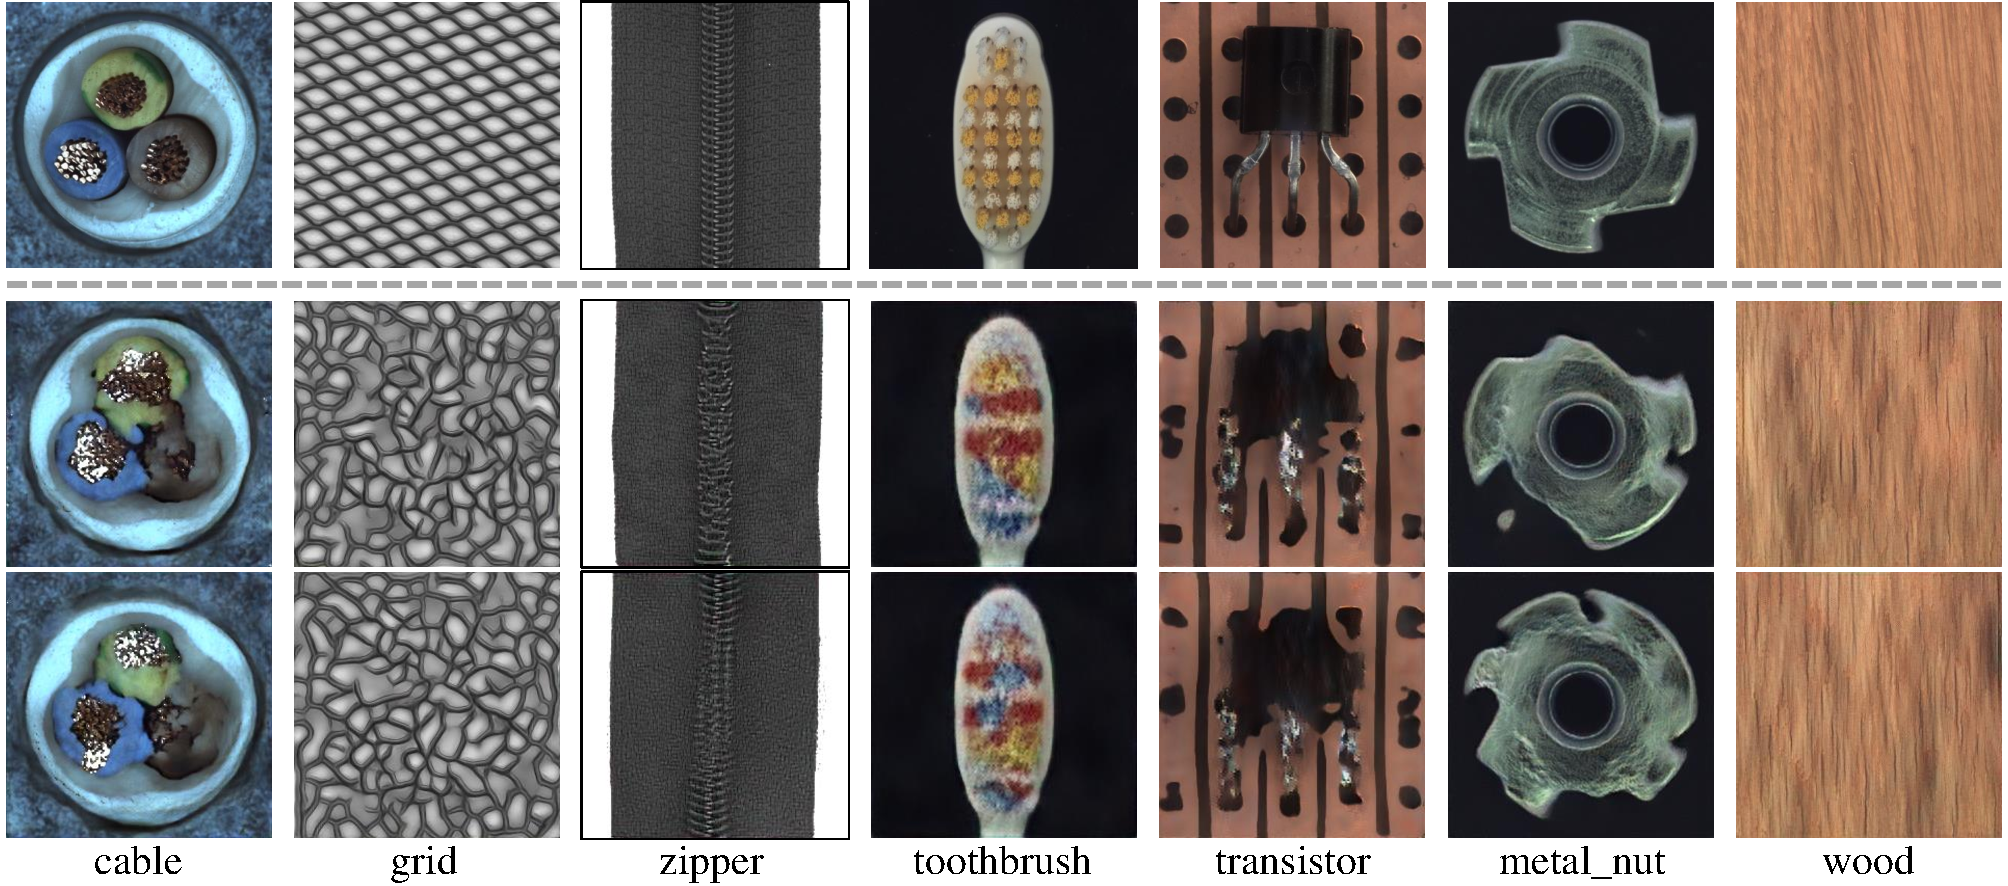
\includegraphics[width=0.7\linewidth]{images/mvtec_generation_results.pdf}
    \caption{Contrastive images generated by level-13 PatchDiff for MVTec AD~\cite{MVTecAD}. } 
    \label{fig: mvtec_generation}
\end{figure*}

\begin{table*}[!h]
    \centering
    % \footnotesize
    % \setlength{\belowcaptionskip}{0.2cm}
    % \setlength{\abovecaptionskip}{0.0cm}
    \renewcommand{\arraystretch}{1.2}
    \resizebox{\textwidth}{!}
    {
\begin{tabular}{cl|c|c|c|c|c|c|c|c}
\toprule
% \multicolumn{2}{c|}{Category} & \makecell[c]{IGD\\\tiny{\citealp{IGD}}} & \makecell[c]{PSVDD\\\tiny{\citealp{PSVDD}}} & \makecell[c]{FCDD\\\tiny{\citealp{FCDD}}} & \makecell[c]{CutPaste\\\tiny{\citealp{CutPaste}}} & \makecell[c]{NSA\\\tiny{\citealp{NSA}}} & \makecell[c]{DRAEM\\\tiny{\citealp{DRAEM}}} & \makecell[c]{DSR\\\tiny{\citealp{DSR}}} & \makecell[c]{GRAD\\\tiny{Ours}} \\ \midrule
\multicolumn{2}{c|}{Category}     & IGD & PSVDD & FCDD & CutPaste &NSA & DRAEM & DSR & GRAD \\ \midrule
\multirow{5}{*}{Texture} 
& carpet & (94.7, 82.8 ) & (92.9, 92.6) & (96.0, - ) & (93.1, 98.3) & (95.5, 95.6) & (95.5,97.0) & (-, \textbf{100.}) & (\textbf{96.5}, 98.2) \\
& grid & (97.7, 97.8 ) & (94.6, 100.) & (91.0, - ) & (\textbf{99.9}, 97.5) & (99.2, 99.9) & (99.7, 99.9) & (-, \textbf{100.}) & (97.2, \textbf{100.}) \\
& leather & (99.5, 95.8) & (90.9, 98.6) & (98.0, - ) & (\textbf{100.}, 99.5) & (99.5, 99.9) & (98.6, \textbf{100.}) & (-, \textbf{100.}) & (98.8, \textbf{100.}) \\
& tile & (78.0, 99.1) & (97.8, 91.4) & (91.0, - ) & (93.4, 90.5) & (\textbf{99.3}, \textbf{100.}) & (99.2, 99.6) & (-, \textbf{100.}) & (95.4, \textbf{100.}) \\
& wood & (89.1, 94.6) & (96.5, 90.8) & (88.0, - ) & (\textbf{98.6}, 95.5) & (90.7, 97.5) & (96.4, \textbf{99.1}) & (-, 96.3) & (87.2, 98.3) \\
\midrule
\multirow{10}{*}{Object} 
& bottle & (92.2, \textbf{100.}) & (98.6, 98.1) & (97.0, - ) & (98.3, 97.6) & (98.3, 97.7) & (\textbf{99.1}, 99.2) & (-, \textbf{100.}) & (96.5, \textbf{100.}) \\
& cable & (84.7, 90.6) & (90.3, 96.8) & (90.0, - ) & (80.6, 90.0) & (96.0, 94.5) & (94.7, 91.8) & (-, 93.8) & (\textbf{98.4}, \textbf{99.3}) \\
& capsule & (\textbf{97.7}, 91.5) & (76.7, 95.8) & (93.0, - ) & (96.2, 97.4) & (97.6, 95.2) & (94.3, \textbf{98.5}) & (-, 98.1) & (97.1, 96.4) \\
& hazelnut & (98.0, 99.7) & (92.0, 97.5) & (95.0, - ) & (97.3, 97.3) & (97.6, 94.7) & (\textbf{99.7}, \textbf{100.}) & (-, 95.6) & (96.6, 98.1) \\
& metal nut & (92.6, 91.3) & (94.0, 98.0) & (94.0, - ) & (99.3, 93.1) & (98.4, 98.7) & (\textbf{99.5}, 98.7) & (-, 98.5) & (93.7, \textbf{100.}) \\
& pill & (97.3, 87.3) & (86.1, 95.1) & (81.0, - ) & (92.4, 95.7) & (\textbf{98.5}, \textbf{99.2}) & (97.6, 98.9) & (-, 97.5) & (98.1, 95.7) \\
& screw & (97.0, 82.5) & (81.3, 95.7) & (86.0, - ) & (86.3, \textbf{96.7}) & (96.5, 90.2) & (97.6, 93.9) & (-, 96.2) & (\textbf{99.2}, 96.0) \\
& toothbrush & (97.7, 99.7) & (\textbf{100.}, 98.1) & (94.0, - ) & (98.3, 98.1) & (94.9, \textbf{100.}) & (98.1, \textbf{100.}) & (-, 99.7) & (98.0, 99.7) \\
& transistor & (84.4, 90.6) & (91.5, 97.0) & (88.0, - ) & (95.5, 93.0) & (88.0, 95.1) & (90.9, 93.1) & (-, 97.8) & (\textbf{97.8}, \textbf{100.}) \\
& zipper & (96.7, 97.0) & (97.9, 95.1) & (92.0, - ) & (\textbf{99.4}, 99.3) & (94.2, 99.8) & (98.9, \textbf{100.}) & (-, \textbf{100.}) & (98.3, 99.7) \\
\midrule
\multicolumn{2}{c|}{Average} & (93.1, 93.4) & (92.5, 93.2 ) & (92.1, 95.7) & (95.2, 96.0) & (96.3, 97.2) & (\textbf{97.3}, 98.0) & (-, 98.2) & (96.8, \textbf{98.7}) \\
\bottomrule
\end{tabular}}
\caption{Anomaly detection performance on MVTec AD dataset~\cite{MVTecAD}. Both pixel-level (left) and image-level (right) AUROC results are shown in each column. The best results are in bold.}
\label{tab: mvtec_main_detail}
\end{table*}

\subsection{Anomaly Detection and Localization}
In the main body, we exclusively present the averaged performance comparison on MVTec AD. In this section, we extend our analysis to provide a detailed result of the anomaly detection and localization performance across each individual sub-dataset within MVTec AD, and display anomaly maps on MVTec AD in Fig.~\ref{fig: main_mvtec_ad_results}. As shown in Table~\ref{tab: mvtec_main_detail}, we compare GRAD to IGD~\cite{IGD}, PSVDD~\cite{PSVDD}, FCDD~\cite{FCDD}, CutPaste~\cite{CutPaste}, NSA~\cite{NSA}, DRAEM~\cite{DRAEM}, and DSR~\cite{DSR}, all of which are independent of pretrained feature extractors. It is easy to find GRAD achieves a strong detection and localization of anomalies.  

\begin{figure*}[!h]
    \centering
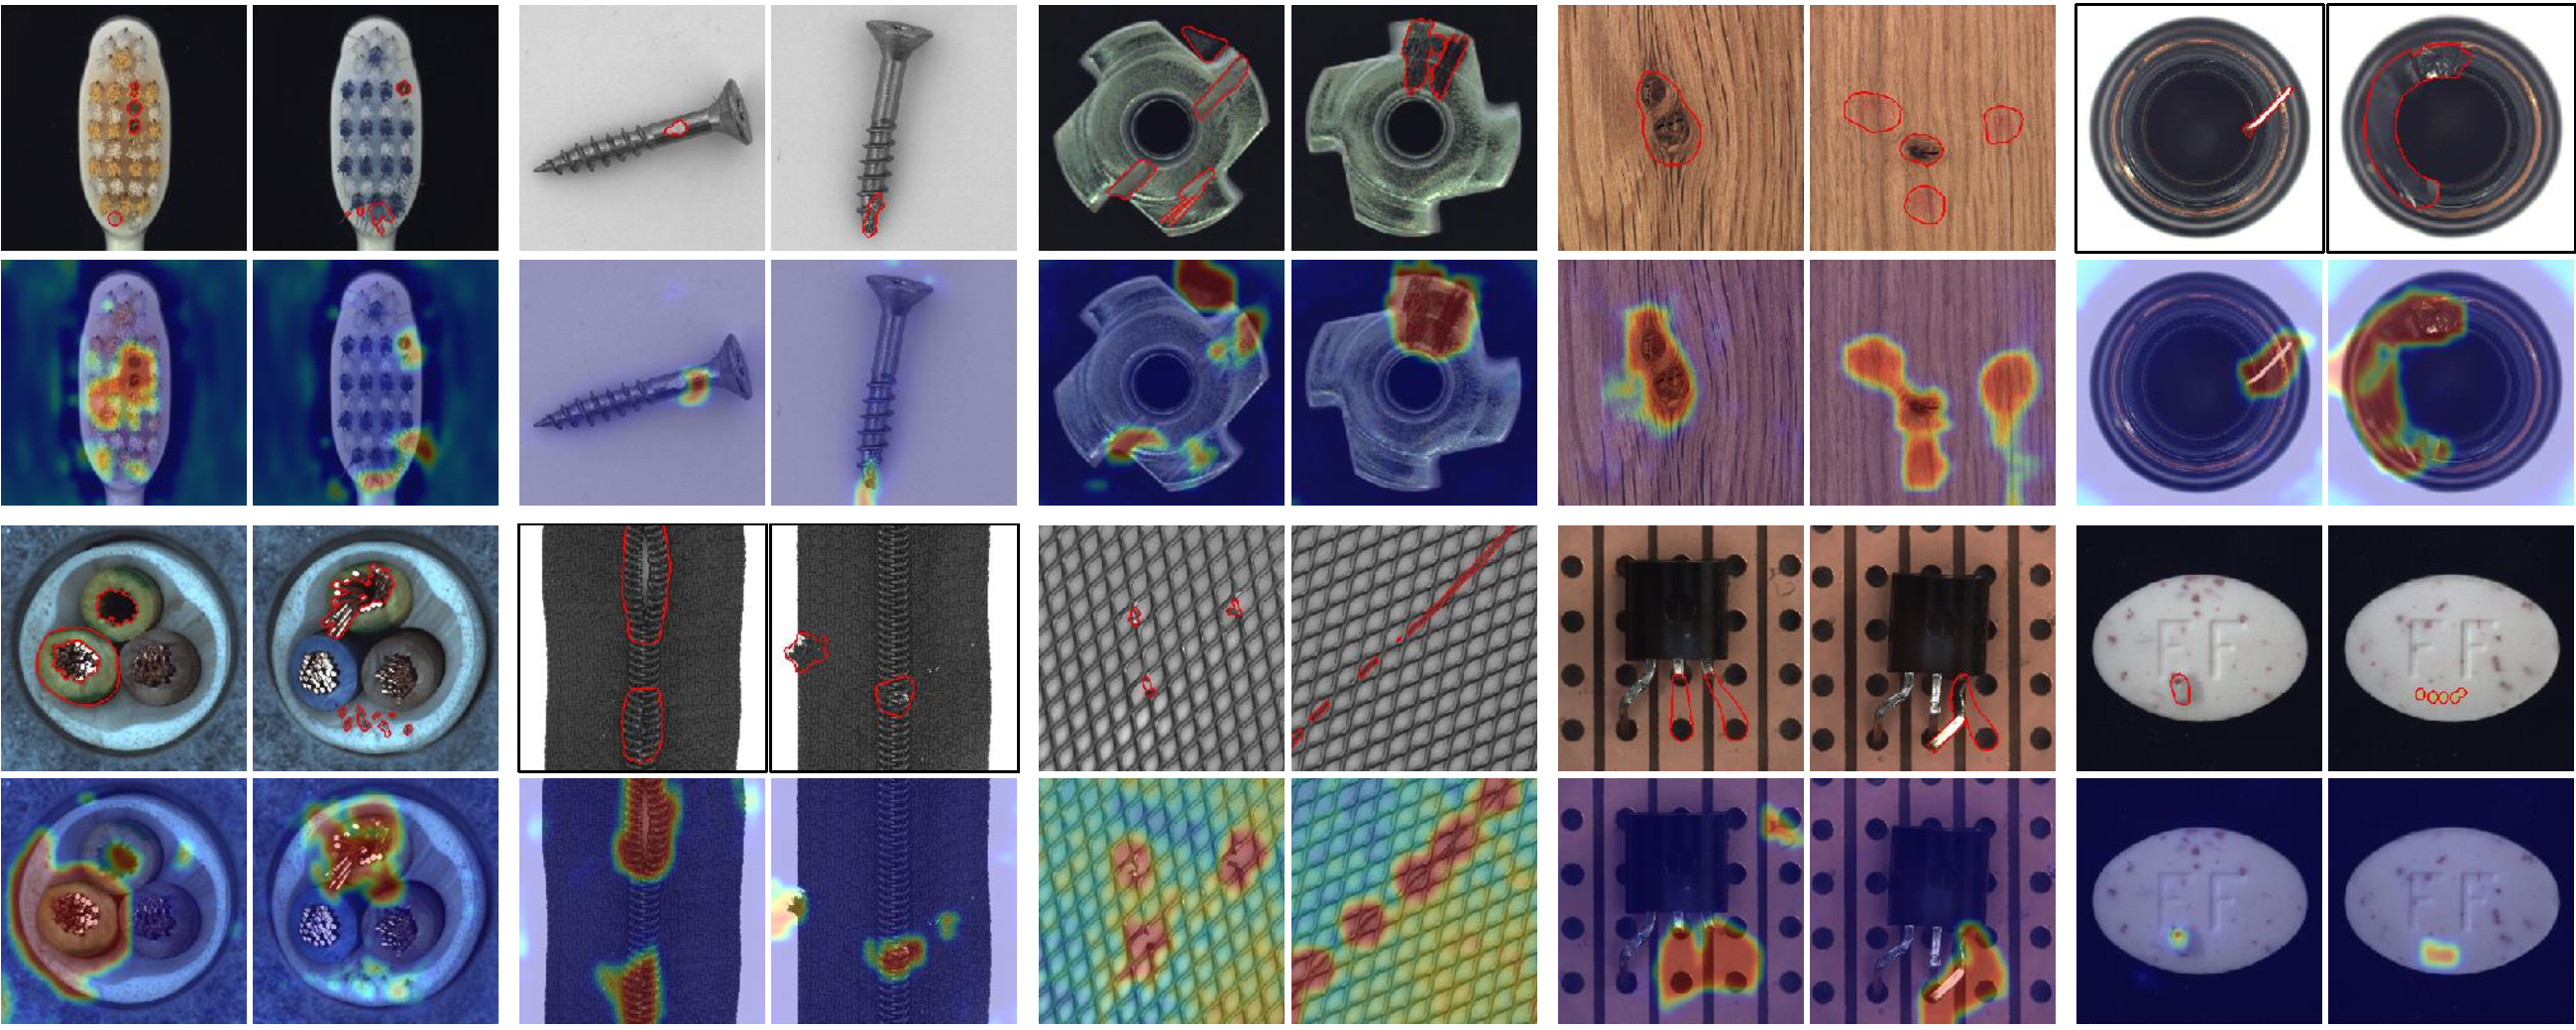
\includegraphics[width=0.9\linewidth]{images/mvtec_results.pdf}
    \caption{Defect localization results of GRAD on MVTec AD~\cite{MVTecAD}. } 
    \label{fig: main_mvtec_ad_results}
    % \vspace{-0.2cm}
\end{figure*}


% In addition, as shown in Table~\ref{tab:ablation_GRad_level}, we conduct an ablations study on selecting levels of patch-level detectors. It is easy to find that when integrating all three different levels of detectors, GRAD can achieve a strong performance for the detection of structural as well as logical anomalies.

% \begin{table}[!htbp]
% \centering
% \footnotesize
% \resizebox{0.3\textwidth}{!}{
% \begin{tabular}{ccc|c}
% \toprule
% \multicolumn{3}{c|}{Level Settings}& Image-level \\
% 136 & 68 & 34  & AUROC\\
% \midrule
% \checkmark &   \ding{55} & \ding{55}   &  85.2   \\
% \ding{55}& \checkmark & \ding{55} & 85.4 \\
% \ding{55}&\ding{55} & \checkmark & 75.1\\
% \checkmark & \checkmark & \ding{55}   &  86.8     \\ %
% \checkmark &   \ding{55} & \checkmark   &  86.4   \\
% \ding{55} & \checkmark & \checkmark  & 86.2 \\
% \checkmark & \checkmark & \checkmark &  \textbf{87.5}  \\
% \bottomrule
% \end{tabular}}
% \caption{Ablation study on detector levels. Detection AUROC results on MVTec LOCO dataset. The best results are in bold.}
% \label{tab:ablation_GRad_level}
% \end{table}



% \bibliography{aaai24}
% \bibliographystyle{aaai24}

% \end{document}



\end{document}
% end of file template.tex

